%%%%%%%%%%%%%%%%%%%%%%%%%%%%%%%%%%%%%%%%%%%%%%%%
%
% Strath PhD Thesis Template
%  by Jethro Browell [jethro.browell@strath.ac.uk]
%
%  Guidelines for thesis format, submission and content are found in
%  General and Course Regulations for Graduate and Postgraduate
%  Awards and Degrees, section 20.6.
%
%  Using .eps or .pdf is recomended to prduce high quality figures etc.
%
%  The Strathclyde logo can be found in other formats at www.strath.ac.uk.
%
%%%%%%%%%%%%%%%%%%%%%%%%%%%%%%%%%%%%%%%%%%%%%%%%

\documentclass[a4paper,oneside,11pt]{book}

\usepackage{amsbsy}
\usepackage{amsmath}
\usepackage{amsfonts}
\usepackage{graphicx}
\usepackage{multirow}
\usepackage{mathrsfs}
\usepackage{xcolor}
\usepackage[hidelinks]{hyperref}
\usepackage{cite}
\usepackage{enumitem}
\usepackage{epsfig}
\usepackage{caption}
\usepackage{subcaption}
\usepackage[strict]{changepage}

\usepackage{amssymb}
\usepackage{amsthm}
\usepackage{catchfilebetweentags}
\usepackage[capitalize]{cleveref}
\usepackage{cmll}
\usepackage{ebproof}
\usepackage[utf8]{inputenc}
\usepackage{mathtools}
\usepackage{mathpartir}
\usepackage{multicol}
\usepackage{newunicodechar}
\usepackage{rotating}
\usepackage{stmaryrd}
\usepackage{todonotes}

\usepackage{tikz}
\usetikzlibrary{cd,fit,matrix,positioning}

\usepackage[conor]{agda}

\theoremstyle{definition}
\newtheorem{theorem}{Theorem}[section]
\newtheorem{conjecture}[theorem]{Conjecture}
\newtheorem{proposition}[theorem]{Proposition}
\newtheorem{lemma}[theorem]{Lemma}
\newtheorem{corollary}[theorem]{Corollary}
\newtheorem{example}[theorem]{Example}
\newtheorem{definition}[theorem]{Definition}
\newtheorem{remark}[theorem]{Remark}

\definecolor{use}{HTML}{008000}
\newcommand\gr[1]{{\color{use}#1}}
\newcommand\grctx[1]{\gr{\mathcal{#1}}}
\newcommand\grP{\grctx P}
\newcommand\grQ{\grctx Q}
\newcommand\grR{\grctx R}
\newcommand\grPprime{\grP\gr'}
\newcommand\grQprime{\grQ\gr'}
\newcommand\name{\ensuremath{\lambda\grR}}
\newcommand\grctxsub[2]{\grctx{#1}_{\gr{#2}}}
\newcommand\grPe{\grctxsub P e}
\newcommand\grPf{\grctxsub P f}
\newcommand\grQe{\grctxsub Q e}
\newcommand\grQf{\grctxsub Q f}
\newcommand\sem[1]{\left\llbracket{#1}\right\rrbracket}
\newcommand\size[1]{\left\lvert{#1}\right\rvert}
\newcommand\ps{\mathit{ps}}
\newcommand\qs{\mathit{qs}}
\newcommand\rs{\mathit{rs}}
\newcommand\dotto{\mathrel{\dot\to}}
\newcommand\dottimes{\mathbin{\dot\times}}
\newcommand\wand{\mathrel{\mathord{-}\hspace{-0.75ex}*}}
\newcommand\sep{\mathbin{*}}
\newcommand\env[1]{(#1\mathrm{-Env})}
\newcommand\thinningN{\mathrm{Thinning}}
\newcommand\thinning[2]{\thinningN~#1~#2}
\newcommand\V{\mathcal V}
\newcommand\C{\mathcal C}
\newcommand\sqin{\mathrel{\mathrlap{\sqsubset}{\mathord{-}}}}
\newcommand\sqni{\mathrel{\mathrlap{\sqsupset}{\mathord{-}}}}
\newcommand\subres{=}
\newcommand\Ann{\mathscr R}

\renewcommand\land{~\wedge~}
\renewcommand\lor{~\vee~}

\DeclareMathOperator\obj{Obj}
\let\hom\relax
\DeclareMathOperator\hom{Hom}
\DeclareMathOperator\id{id}
\DeclareMathOperator\sub{Sub}

\usepackage[T1]{fontenc}

\newunicodechar{λ}{\ensuremath{\mathnormal\lambda}}
\newunicodechar{ρ}{\ensuremath{\mathnormal\rho}}
\newunicodechar{→}{\ensuremath{\mathnormal\to}}
\newunicodechar{∀}{\ensuremath{\mathnormal\forall}}
\newunicodechar{ι}{\ensuremath{\mathnormal\iota}}
\newunicodechar{·}{\ensuremath{\mathnormal\cdot}}
\newunicodechar{⊸}{\ensuremath{\mathnormal\multimap}}
\newunicodechar{⊕}{\ensuremath{\mathnormal\oplus}}
\newunicodechar{─}{\textrm{---}}
\newunicodechar{│}{\ensuremath{\mid}}
\newunicodechar{ᶜ}{\ensuremath{\mathnormal{^c}}}
\newunicodechar{ᵉ}{\ensuremath{\mathnormal{^e}}}
\newunicodechar{ᵏ}{\ensuremath{\mathnormal{^k}}}
\newunicodechar{ₗ}{\ensuremath{\mathnormal{_l}}}
\newunicodechar{ₘ}{\ensuremath{\mathnormal{_m}}}
\newunicodechar{ₙ}{\ensuremath{\mathnormal{_n}}}
\newunicodechar{ᵣ}{\ensuremath{\mathnormal{_r}}}
\newunicodechar{ʳ}{\ensuremath{\mathnormal{^r}}}
\newunicodechar{ˢ}{\ensuremath{\mathnormal{^s}}}
\newunicodechar{ᵗ}{\ensuremath{\mathnormal{^t}}}
\newunicodechar{ᵛ}{\ensuremath{\mathnormal{^v}}}
\newunicodechar{ᴹ}{\ensuremath{\mathnormal{^M}}}
\newunicodechar{↙}{\ensuremath{\mathnormal\swarrow}}
\newunicodechar{↘}{\ensuremath{\mathnormal\searrow}}
\newunicodechar{⊢}{\ensuremath{\mathnormal\vdash}}
\newunicodechar{⊨}{\ensuremath{\mathnormal\vDash}}
\newunicodechar{⟦}{\ensuremath{\mathnormal\llbracket}}
\newunicodechar{⟧}{\ensuremath{\mathnormal\rrbracket}}
\newunicodechar{✴}{\ensuremath{\mathnormal*}}
\newunicodechar{ℓ}{\ensuremath{\mathnormal\ell}}
\newunicodechar{Γ}{\ensuremath{\mathnormal\Gamma}}
\newunicodechar{γ}{\ensuremath{\mathnormal\gamma}}
\newunicodechar{Δ}{\ensuremath{\mathnormal\Delta}}
\newunicodechar{δ}{\ensuremath{\mathnormal\delta}}
\newunicodechar{Θ}{\ensuremath{\mathnormal\Theta}}
\newunicodechar{Σ}{\ensuremath{\mathnormal\Sigma}}
\newunicodechar{σ}{\ensuremath{\mathnormal\sigma}}
\newunicodechar{∈}{\ensuremath{\mathnormal\in}}
\newunicodechar{∋}{\ensuremath{\mathnormal\ni}}
\newunicodechar{′}{\ensuremath{\mathnormal'}}
\newunicodechar{≡}{\ensuremath{\mathnormal\equiv}}
\newunicodechar{⊤}{\ensuremath{\mathnormal\top}}
\newunicodechar{⊥}{\ensuremath{\mathnormal\bot}}
\newunicodechar{▹}{\ensuremath{\mathnormal\triangleright}}
\newunicodechar{₁}{\ensuremath{\mathnormal{_1}}}
\newunicodechar{□}{\ensuremath{\mathnormal\Box}}
\newunicodechar{○}{\ensuremath{\mathnormal\bigcirc}}
\newunicodechar{𝓒}{\ensuremath{\C}}
\newunicodechar{𝓥}{\ensuremath{\V}}
\newunicodechar{∘}{\ensuremath{\mathnormal\circ}}
\newunicodechar{≤}{\ensuremath{\mathnormal\leq}}
\newunicodechar{◇}{\ensuremath{\mathnormal\diamond}}
\newunicodechar{ℕ}{\ensuremath{\mathbb N}}
\newunicodechar{⁺}{\ensuremath{\mathnormal{^+}}}
\newunicodechar{⊔}{\ensuremath{\mathnormal\sqcup}}
\newunicodechar{⇒}{\ensuremath{\mathnormal\Rightarrow}}

% Characters that are different from what appears in the source code
\newunicodechar{ℑ}{\ensuremath{\mathnormal{I^*}}}
\newunicodechar{⇛}{\ensuremath{\mathnormal{\Longrightarrow}}}
\newunicodechar{∩}{\ensuremath{\mathnormal\dottimes}}
\newunicodechar{∧}{\ensuremath{\mathnormal\dottimes}}
\newunicodechar{⒈}{\ensuremath{\mathnormal{\dot1}}}
\newunicodechar{⇴}{\ensuremath{\mathnormal\dotto}}
\newunicodechar{⇥}{\ensuremath{\mathnormal\wand}}


% Page Margins - Strath Requirement
\usepackage[left=4cm,right=2.5cm,top=2cm,bottom=4cm,includehead,includefoot,headheight=15pt]{geometry}

% Page Headers
\usepackage{fancyhdr}
\fancyhf{}
\renewcommand{\headrulewidth}{0pt} % optional
%\fancyhead[L]{\nouppercase{\leftmark} \hfill Section \nouppercase{\rightmark}}
\fancyhead[L]{\nouppercase{\leftmark}}
\cfoot{\thepage}
\pagestyle{fancy}

% Draft Watermark
%\usepackage[draft=true,allpages=true,fontfamily=cmr,angle=90,scale=0.1,mark={\fboxsep=35pt\fboxrule=0pt\relax\fbox{-- DRAFT -- \today~--}},xcoord=-80,ycoord=-20]{draftwatermark}


% Line Spacing
%\def\baselinestretch{1.5}
\usepackage{setspace}
\setstretch{1.5}


% Place UoS Logo on Title Page (this package modifies the "\maketitel" command.)
\usepackage{titling}
\pretitle{%
  \begin{flushright}
  \vspace{-9.5cm}
%  \includegraphics[width=5cm,natwidth=472,natheight=531]{logo} \\[7cm]
  \includegraphics[width=5cm]{logo} \\[6cm]
  \end{flushright}
  \begin{center}
  \LARGE
}
\posttitle{\end{center}}

\title{Variables in Quantitative Type Theories \\ PhD Thesis}
\author{James Wood
\\ \small Mathematically Structured Programming\\[-0.8ex]
\small Computer and Information Sciences\\[-0.8ex]
\small University of Strathclyde, Glasgow\\
}




%%%%%%%%%%%%%%%%%%%%%%%%%%%%%%%%%%%%%%%%%%%%%%%%%%%%%%%%%%%%%%
\begin{document}

\maketitle


%%%%%%%%%%%%%%%%%%%%%%%%%%%%%%%%%%%%%%%%%%%%%%%%%%%%%%%%%%%%%%
\frontmatter
%%%%%%%%%%%%%%%%%%%%%%%%%%%%%%%%%%%%%%%%%%%%%%%%%%%%%%%%%%%%%%

% Declaration
\topskip0pt
\vspace*{\fill}
\noindent
\begin{quote}
  \centering
  This thesis is the result of the author's original research. It has been composed by the author and has not been previously submitted for examination which has led to the award of a degree. \\[5pt]
  %
  The copyright of this thesis belongs to the author under the terms of the United Kingdom Copyright Acts as qualified by University of Strathclyde Regulation 3.50. Due acknowledgement must always be made of the use of any material contained in, or derived from, this thesis. \\[5pt]
  %
  %Signed: \\
  %Date:
\end{quote}
\vspace*{\fill}



\chapter{Abstract}



\tableofcontents

\addcontentsline{toc}{chapter}{List of Figures}
\listoffigures

\addcontentsline{toc}{chapter}{List of Tables}
\listoftables



\chapter{Preface/Acknowledgements}
I would like to acknowledge...

This document is adapted from the template by Jethro Browell
(\url{https://www.overleaf.com/latex/templates/thesis-template-for-university-of-strathclyde/nfnrnmjqyxqg}),
which was licensed under CC BY 4.0.



%%%%%%%%%%%%%%%%%%%%%%%%%%%%%%%%%%%%%%%%%%%%%%%%%%%%%%%%%%%%%%
\mainmatter
%%%%%%%%%%%%%%%%%%%%%%%%%%%%%%%%%%%%%%%%%%%%%%%%%%%%%%%%%%%%%%


\chapter{Introduction}

\chapter{Mathematical preliminaries}
  Categories, (co)products, monoidal categories, string diagrams (in Rel),
  monoid objects.
  Examples: Set, Rel, partial functions, commutative monoids.

\chapter{Linearity}
  \section{Intuitionistic linear logic}
  Linear logic is a good starting point for our investigations into usage
restrictions because it is well known, well understood, and exhibits most of the
difficulties we will come across.
Linear logic's lack of general weakening and contraction will be a typical
feature of the calculi we will see, and the exponential modality $\oc$ (bang)
will be the prototype for a range of modalities I will consider.

\subsection{Motivation of linearity}

While classical linear logic is perhaps better understood, for the sake of this
thesis I focus on intuitionistic linear logic.
The syntactic difference between the two is analogous to the difference between
classical and intuitionistic logic: The latter restricts the former by only
allowing one formula on the right of a sequent.
Classical linear logic is not irrelevant to this thesis, and appears as an
instance of the framework presented in \cref{sec:framework}.
However, the connection of this work to intuitionistic linear logic is more
direct, and reflects the basis of existing semiring-annotated calculi on
(intuitionistic) typed $\lambda$-calculi.

Intuitionistic linear logic is often motivated by its sensitivity to resources.
The fact that, in intuitionistic (and classical) logic, \emph{any} hypothesis
can be discarded or duplicated means that propositions cannot be used to model
things that may be ``possessed'' or ``spent'', despite hypotheses often being
described as things we ``have''.
In contrast, linear logic allows propositions to behave like physical objects,
being moved around but not being created or destroyed (a priori).

Programming applications of linearity include stateful protocols
\citep{Wadler12}, mutually exclusive capabilities (TODO: cite),
and mutation (TODO: cite).
In each of these cases, the act of using up a hypothesis allows us to divide
time into ``before'' and ``after'', with lack of duplication avoiding confusion
over which half we are in, and lack of deletion allowing us to know whether the
corresponding action actually happened.
For example, when modelling mutation, a variable refers to a single state of a
mutable value.
The \texttt{write} operation uses up such a variable, making the old state
inaccessible, and returns a new linear value to represent the new state of the
mutable value.
Such a protocol naturally also supports a \emph{freezing} operation, by which we
relinquish the ability to mutate the value in return for an immutable reference
to the value produced.

%In LJ, two distinct, but equiderivable, canonical definitions of $\wedge$ can
%be given.
%
%In the first approach, $\wedge^-$ is conceived to be a
%\emph{categorial product}.
%Such a product is constructed by providing two maps in from the same antecedents
%$\Gamma$.
%It is used by projecting out one of the sides.
%
%\begin{mathpar}
%  \inferrule*[right=$\wedge^-$-r]
%  {\Gamma \vdash A \\ \Gamma \vdash B}
%  {\Gamma \vdash A \wedge^- B}
%
%  \and
%
%  \inferrule*[right=$\wedge^-$-l$_0$]
%  {\Gamma, A \vdash C}
%  {\Gamma, A \wedge^- B \vdash C}
%
%  \and
%
%  \inferrule*[right=$\wedge^-$-l$_1$]
%  {\Gamma, B \vdash C}
%  {\Gamma, A \wedge^- B \vdash C}
%\end{mathpar}
%
%In the second approach, $\wedge^+$ is conceived to be a \emph{tensor product}.
%Intuitively, $\wedge^+$ internalises the comma of context concatenation.
%Such a product is used by giving access to both sides simultaneously.
%It is constructed by constructing both sides and combining the antecedents
%required by each side.
%
%\begin{mathpar}
%  \inferrule*[right=$\wedge^+$-r]
%  {\Gamma \vdash A \\ \Delta \vdash B}
%  {\Gamma, \Delta \vdash A \wedge^+ B}
%
%  \and
%
%  \inferrule*[right=$\wedge^+$-l]
%  {\Gamma, A, B \vdash C}
%  {\Gamma, A \wedge^+ B \vdash C}
%\end{mathpar}
%
%When we prove the logical equivalence of these two formulations, we notice that
%the structural rules of weakening and contraction are essential.
%When we remove weakening and contraction, $\wedge^-$ and $\wedge^+$ become
%logically distinct connectives, which we notate $\&$ and $\otimes$,
%respectively.
%
%\begin{mathpar}
%  \inferrule*[right=$\wedge^-$-r]
%  {%
%    \inferrule*[right=Weak$^*$,fraction={\cdot\cdots\cdot}]
%    {\Gamma \vdash A}
%    {\Gamma, \Delta \vdash A}
%    \\
%    \inferrule*[Right=Weak$^*$,fraction={\cdot\cdots\cdot}]
%    {\Delta \vdash B}
%    {\Gamma, \Delta \vdash B}
%  }
%  {\Gamma, \Delta \vdash A \wedge^- B}
%
%  \and
%
%  \inferrule*[right=Contr]
%  {%
%    \inferrule*[Right=$\wedge^-$-l$_0$]
%    {%
%      \inferrule*[Right=$\wedge^-$-l$_1$]
%      {\Gamma, A, B \vdash C}
%      {\Gamma, A, A \wedge^- B \vdash C}
%    }
%    {\Gamma, A \wedge^- B, A \wedge^- B \vdash C}
%  }
%  {\Gamma, A \wedge^- B \vdash C}
%\end{mathpar}
%
%\begin{mathpar}
%  \inferrule*[right=Contr$^*$,fraction={\cdot\cdots\cdot}]
%  {%
%    \mprset{defaultfraction}
%    \inferrule*[Right=$\wedge^+$-r]
%    {\Gamma \vdash A \\ \Gamma \vdash B}
%    {\Gamma, \Gamma \vdash A \wedge^+ B}
%  }
%  {\Gamma \vdash A \wedge^+ B}
%
%  \and
%
%  \inferrule*[right=$\wedge^+$-l]
%  {%
%    \inferrule*[Right=Weak]
%    {\Gamma, A \vdash C}
%    {\Gamma, A, B \vdash C}
%  }
%  {\Gamma, A \wedge^+ B \vdash C}
%
%  \and
%
%  \inferrule*[right=$\wedge^+$-l]
%  {%
%    \inferrule*[Right=Weak]
%    {\Gamma, B \vdash C}
%    {\Gamma, A, B \vdash C}
%  }
%  {\Gamma, A \wedge^+ B \vdash C}
%\end{mathpar}

\subsection{The multiplicative-additive fragment}

The multiplicative-additive fragment of linear logic (MALL) is the fragment
where all hypotheses are linear (must be used exactly once).
We will extend MALL with the \emph{exponential} modality in
\cref{sec:bang-modality}.
MALL is unable to embed intuitionistic or classical logic (collectively
known as \emph{structural logics}), as MALL is unable to reflect any of the
discarding or duplication that can be done in proofs in structural logics.

In short, the syntax of intuitionistic MALL can be described as intuitionistic
logic with the structural rules of \emph{weakening} and \emph{contraction}
removed.
However, without the presence of weakening and contraction, we have to be more
careful about the rules we state, so as not to accidentally introduce weakening
and contraction admissibly.
The lack of these structural rules also allows us to observe a new phenomenon:
the distinction (at the level of provability) between \emph{additive} and
\emph{multiplicative} formulations of existing connectives (in particular, in
the intuitionistic case, the conjunction connective).

I present MALL in \cref{fig:mall} in a sequent calculus style, as it was
presented by \citet{girard87linear}.

To encode what it means to use a hypothesis \emph{exactly once}, we first need
to decide what counts as a use.
The simplest case is that the identity sequent counts as a single use of its
sole hypothesis, and conversely does not count as a use of any other hypotheses.
For sequential proofs, created by the \TirName{Cut} rule, if we have a proof of
$A$ using $\Gamma$, and a proof of $B$ using $\Delta$ and $A$, then we have a
proof of $B$ transitively using $\Delta$ and $\Gamma$.
The exchange rule Exch says that use is invariant under permutation.

For the logical connectives, we have genuine choices as to what it means to use
them.
Two cases --- disjunction ($\oplus$) and (linear) implication ($\multimap$) ---
are somewhat intuitive from intuitionistic logic.
A canonical proof of a disjunction is a tag and a proof of one of the two
disjuncts.
This suggests that a proof of a disjunction only uses the same hypotheses as
the proof of the disjunct we actually choose, with the other disjunct being
irrelevant.
Correspondingly, when we use a disjunction hypothesis, we will only actually use
one of the cases, so each branch should use the same hypotheses.
For implication, use is sequential like with the \TirName{Cut} rule, and its
left rule is more or less the only choice that allows use of the surrounding
hypotheses.

For conjunction, there are two choices: Either the conjuncts \emph{together} use
all of the hypotheses, or each of the conjuncts \emph{individually} uses all of
the hypotheses.
The former choice gives us the tensor-product ($\otimes$), and the latter choice
gives us the with-product ($\with$).
These products are equivalent up to provability in structural logics but
distinct in linear logic.

\begin{figure}
  \begin{align*}
    A, B, C &\Coloneqq X \mid I \mid A \otimes B \mid A \multimap B
              \mid 0 \mid A \oplus B \mid \top \mid A \with B \\
    \Gamma, \Delta, \Theta &\Coloneqq {\cdot} \mid \Gamma, A
  \end{align*}
  \begin{mathpar}
    \ebrule{%
      \infer0[Id]{A \vdash A}
    }

    \and

    \ebrule{%
      \hypo{\Gamma \vdash A}
      \hypo{\Delta, A \vdash B}
      \infer2[Cut]{\Gamma, \Delta \vdash B}
    }

    \and

    \ebrule{%
      \hypo{\Gamma, B, A, \Delta \vdash C}
      \infer1[Exch]{\Gamma, A, B, \Delta \vdash C}
    }

    \and

    \ebrule{%
      \hypo{\Gamma \vdash C}
      \infer1[$I$-L]{\Gamma, I \vdash C}
    }

    \and

    \ebrule{%
      \infer0[$I$-R]{{\cdot} \vdash I}
    }

    \and

    \ebrule{%
      \hypo{\Gamma, A, B \vdash C}
      \infer1[$\otimes$-L]{\Gamma, A \otimes B \vdash C}
    }

    \and

    \ebrule{%
      \hypo{\Gamma \vdash A}
      \hypo{\Delta \vdash B}
      \infer2[$\otimes$-R]{\Gamma, \Delta \vdash A \otimes B}
    }

    \and

    \ebrule{%
      \hypo{\Gamma \vdash A}
      \hypo{\Delta, B \vdash C}
      \infer2[$\multimap$-L]{\Gamma, \Delta, A \multimap B \vdash C}
    }

    \and

    \ebrule{%
      \hypo{\Gamma, A \vdash B}
      \infer1[$\multimap$-R]{\Gamma \vdash A \multimap B}
    }

    \and

    \ebrule{%
      \infer0[$0$-L]{\Gamma, 0 \vdash C}
    }

    \and

    \text{(no $0$-R)}

    \and

    \ebrule{%
      \hypo{\Gamma, A \vdash C}
      \hypo{\Gamma, B \vdash C}
      \infer2[$\oplus$-L]{\Gamma, A \oplus B \vdash C}
    }

    \and

    \ebrule{%
      \hypo{\Gamma \vdash A_i}
      \infer1[$\oplus$-R$_i$]{\Gamma \vdash A_0 \oplus A_1}
    }

    \and

    \text{(no $\top$-L)}

    \and

    \ebrule{%
      \infer0[$\top$-R]{\Gamma \vdash \top}
    }

    \and

    \ebrule{%
      \hypo{\Gamma, A_i \vdash C}
      \infer1[$\with$-L$_i$]{\Gamma, A_0 \with A_1 \vdash C}
    }

    \and

    \ebrule{%
      \hypo{\Gamma \vdash A}
      \hypo{\Gamma \vdash B}
      \infer2[$\with$-R]{\Gamma \vdash A \with B}
    }
  \end{mathpar}
  \caption{Multiplicative-additive fragment of linear logic}
  \label{fig:mall}
\end{figure}

Implication ($\multimap$) and the tensor-product ($\otimes$, $I$) comprise the
\emph{multiplicative} fragment, while disjunction ($\oplus$, $0$) and the
with-product ($\with$, $\top$) comprise the \emph{additive} fragment.
Categorically, the additive fragment corresponds to products and coproducts,
while the multiplicative fragment corresponds to multicategorical tensor
products and closure.

\subsection{The $\oc$-modality}\label{sec:bang-modality}

\begin{mathpar}
  \ebrule{%
    \hypo{\oc\Gamma \vdash A}
    \infer1[Promotion]{\oc\Gamma \vdash \oc A}
  }

  \and

  \ebrule{%
    \hypo{\Gamma, A \vdash B}
    \infer1[Dereliction]{\Gamma, \oc A \vdash B}
  }

  \and

  \ebrule{%
    \hypo{\Gamma \vdash B}
    \infer1[Weakening]{\Gamma, \oc A \vdash B}
  }

  \and

  \ebrule{%
    \hypo{\Gamma, \oc A, \oc A \vdash B}
    \infer1[Contraction]{\Gamma, \oc A \vdash B}
  }
\end{mathpar}

In the intuitionistic linear logic sequent calculus ILL, $\oc A$ is defined
to be a proposition whose occurrences as antecedents can be deleted
(\TirName{Weakening}) and duplicated (\TirName{Contraction}), from which we can
extract $A$ (\TirName{Dereliction}), and which we can form from a conclusion
$A$ only when all antecedents are of the form $\oc X$ for some proposition $X$
(\TirName{Promotion}).
In short, $\oc A$ can be seen as an intuitionistic version of $A$, supporting
all of the structural rules of LJ, and only being able to be formed when it
does not depend on anything linear.

While this definition of $\oc$ works, in the sense that it gives the intended
class of models and cut elimination is maintained, it has some disadvantages.
Firstly, while the multiplicative and additive connectives are all characterised
by universal properties, $\oc$ is not.
This can be seen by the fact that taking the rules for $\oc$ and replacing each
occurrence of $\oc$ by a fresh connective $\oc'$ produces a logically distinct
connective.
One cannot produce any derivation of $\oc' A \vdash \oc A$ because
\TirName{Promotion} does not apply when there are antecedents not of the form
$\oc X$.
Finally, while $\oc$ is supposed to be a positive connective, it sometimes
behaves like a negative connective.
For example, for a positive connective like $\otimes$, the normal form proof
of the identity sequent $P \otimes Q \vdash P \otimes Q$ starts (from the
bottom) with a left rule and then, with the left in a more amenable form,
applies the right rule.
In contrast, the normal form proof of $\oc P \vdash \oc P$ starts with the
right rule, as it needs to have everything on the left be of the form $\oc X$.

\begin{mathpar}
  \ebrule{%
    \infer0[Id]{P \vdash P}
    \infer0[Id]{Q \vdash Q}
    \infer2[$\otimes$-r]{P, Q \vdash P \otimes Q}
    \infer1[$\otimes$-l]{P \otimes Q \vdash P \otimes Q}
  }

  \and

  \ebrule{%
    \infer0[Id]{P \vdash P}
    \infer1[Der]{\oc P \vdash P}
    \infer1[Pro]{\oc P \vdash \oc P}
  }
\end{mathpar}

  \section{DILL}
  DILL provides a syntax in which $\oc$ is characterised by a universal
  property.
  There is no need for any rule to depend on the entire context and rebind
  variables (as done by BBdPH), so is more ND-like.
  DILL makes $\oc$ behave more like a positive type former (see the deep
  identity function $\oc A \vdash \oc A$).
  DILL has been extended to dependent types: Vakar15.

  The idea of split contexts can also be applied to left-/right-rule systems.
  (Define this DILL variant.)

  \section{Mechanisation survey}

  %\section{Notice what additive/multiplicative/exponential rules look like}

\chapter{Mechanisation of simple types}
  \section{Term representation}
  We could mechanise Gentzen's definition of a natural deduction system directly,
but this definition is quite complicated.
In particular, if we want to give derivations an inductive definition, the use
of the discharge mechanism means that we actually need an inductive-inductive
type --- derivations, particularly those using $\to$-introduction, can involve
references to assumptions within their subderivations.
An inductive-inductive definition of derivations would complicate our programs
and proofs about natural deduction derivations, so I choose an alternative
representation.

Indeed, most authors since Gentzen, whether mechanising their work or not,
have opted to replace discharge of assumptions by explicit \emph{contexts} and
a variable rule.
Contexts can be justified as a way to keep track of undischarged assumptions.
In particular, we only produce derivations in the presence of a known collection
of \emph{free variables} specified by the context.
In other words, derivations are \emph{indexed} over their free variables and
their types.
When using an assumption within a derivation, we must say which free variable
it corresponds to.
Free variables are introduced by \emph{variable-binding} rules, like
$\to$-introduction.
\cref{fig:explicit-contexts} gives an example of the same derivation written
in Gentzen's style and in the explicit context style.

\begin{sidewaysfigure}
  \centering
  \begin{prooftree}
    \hypo{[A \to A \to B]^f}
    \hypo{[A]^x}
    \infer2[$\to$-E]{A \to B}
    \hypo{[A]^x}
    \infer2[$\to$-E]{B}
    \infer1[$\to$-I$^x$]{A \to B}
    \infer1[$\to$-I$^f$]{\plr{A \to A \to B} \to \plr{A \to B}}
  \end{prooftree}

  \vspace{2em}

  \begin{prooftree}
    \infer0[var$^f$]{{\color{red}f : A \to A \to B, x : A} \vdash A \to A \to B}
    \infer0[var$^x$]{{\color{red}f : A \to A \to B, x : A} \vdash A}
    \infer2[$\to$-E]{{\color{red}f : A \to A \to B, x : A} \vdash A \to B}
    \infer0[var$^x$]{{\color{red}f : A \to A \to B, x : A} \vdash A}
    \infer2[$\to$-E]{{\color{red}f : A \to A \to B, x : A} \vdash B}
    \infer1[$\to$-I$^x$]{{\color{red}f : A \to A \to B} \vdash A \to B}
    \infer1[$\to$-I$^f$]{\vdash \plr{A \to A \to B} \to \plr{A \to B}}
  \end{prooftree}
  \caption{A proof in Gentzen's natural deduction syntax, and a proof using
    explicit contexts (contexts coloured {\color{red}red})}
  \label{fig:explicit-contexts}
\end{sidewaysfigure}

Explicit contexts can be seen as a mechanism for encoding a natural deduction
system as a sequent calculus.
However, the natural deduction character of the system is maintained by
ensuring that the resultant sequent calculus is really an encoding of a
natural deduction system.
Concretely, this means that rules can only interact with the context in
restricted ways:

\begin{itemize}
  \item There is a designated \emph{variable rule}, stating that any variable
    in the context can serve as a derivation of its type.
  \item Non-variable rules may only require subterms with \emph{extended}
    contexts, i.e., subterms in which new variables have been bound.
    Non-variable rules are parametric in the existing free variables.
\end{itemize}

Having chosen to use explicit contexts, the mechanisation must have a chosen
representation of contexts as a data structure.
While the notation in \cref{fig:explicit-contexts} uses names $f$ and $x$
for variables, I opt for a nameless representation.
In a nameless representation, variables are identified by their position in
the context, rather than by a name.
The absence of names means that $\alpha$-equivalence is just on-the-nose
equality, and also that we never have to reason about freshness of names.
Agda does not have support for nominal techniques~\cite{GP02}, which may have
made names a better option.

Most mechanisations choose contexts to be an inductive list of types.
However, I instead choose a functional, tree-shaped representation, as shown
with the type \AgdaRecord{Ctx}.
The type \AgdaDatatype{LTree} is the inductive type generated by leaves and
nullary \& binary nodes, and serves as a generalised ``length'' of the context.
The tree shape makes concatenation definitionally
injective, so that in cases where multiple new variables are bound in a subterm
(for example, $\otimes$-elimination), Agda's unification-based solving will
be more able to infer which variables have just been bound.
Within a given \AgdaBound{t}\AgdaSpace{}\AgdaSymbol:\AgdaSpace{}%
\AgdaDatatype{LTree}, we can define the positions of \AgdaBound{t} using
\AgdaDatatype{Ptr}.
A \emph{pointer} (\AgdaDatatype{Ptr}) into a tree picks out a leaf
(\AgdaInductiveConstructor{[-]}) following a path of lefts
(\AgdaInductiveConstructor{$\swarrow$}) and rights
(\AgdaInductiveConstructor{$\searrow$}) at any binary nodes encountered.

\ExecuteMetaData[\LTreetex]{LTree}
\ExecuteMetaData[\LTreetex]{Ptr}

The contents of the context --- the types --- are then stored in the functional
vector \AgdaField{ty-ctx}, which is a mapping from leaves in \AgdaField{shape}
to object language types \AgdaDatatype{Ty}.
The advantages of the functional vector representation will not become clear
until later chapters --- particularly the example in
\cref{sec:usage-elaborator}, where I make use of the ease of look-up and the
$\eta$-law of functions.
However, I claim for now that there is little to no disadvantage in the
functional vector representation --- in particular, we have no need for
function extensionality principles because we never talk about equality of
contexts.
For example, instead of using an equality of contexts to coerce a term, we can
use renaming.

\ExecuteMetaData[\Vectortex]{Vector}
\Ctx{}

Our first data structure involving contexts is that of intrinsically typed
variables.
A variable of type
\AgdaBound{$\Gamma$}\AgdaSpace{}\AgdaRecord{$\ni$}\AgdaSpace{}\AgdaBound{A}
is given by a path \AgdaField{idx} to a type in \AgdaBound{$\Gamma$}, together
with a proof \AgdaField{tyq} that this type is equal to \AgdaBound{A}.

\Var{}

Variables embed into terms via the \AgdaInductiveConstructor{var} constructor of
the family \AgdaDatatype{\_⊢\_} of intrinsically simply typed terms.
The only other syntactic forms we consider for now are the eliminator and
constructor of function types \AgdaInductiveConstructor{\_`→\_} ---
\AgdaInductiveConstructor{app} and \AgdaInductiveConstructor{lam}.
Application \AgdaInductiveConstructor{app} takes two subterms of the appropriate
types, while the subterm of $\lambda$-abstraction \AgdaInductiveConstructor{lam}
is in an extended context \GA{} --- \AgdaBound{$\Gamma$} concatenated with a
singleton context containing the type \AgdaBound{A}.

\Term{}

Using this encoding, the Church numeral for 2 appears as follows.
In standard notation, this would be
$\lambda f.~\lambda x.~f\,(f\,x)$.
To refer to $f$ in the main body of the expression, we skip one binder (using
\AgdaInductiveConstructor{$\swarrow$}) and pick the next one
(using \AgdaInductiveConstructor{$\searrow$}) and pick its only bound variable
(using \AgdaInductiveConstructor{here}).
To refer to $x$, we do not skip its binder, instead picking it and its only
bound variable.

\ExecuteMetaData[../agda/processed-latex/SimpleKits.tex]{two}

  \section{Renaming and substitution}\label{sec:kits}
  \def\SimpleKits{../agda/processed-latex/SimpleKits.tex}

%Explain:
%
%\begin{itemize}
%  \item Specific uses of renaming/substitution in $\lambda$-calculus semantics.
%  \item General role of renaming/substitution in abstract algebra/syntax with
%    binding.
%\end{itemize}

A basic operation on any syntax with variables is \emph{substitution} --- the
replacement of variables in a term by terms with the same type as the variables.
In a sense, this is the defining operation of variables --- a variable is a
placeholder for a term, or equivalently in logic, a hypothesis is a placeholder
for an arbitrary proof.
In a type theory or logic, terms can bind variables, and we will typically have
operational semantics rules combining a term binding a variable with a term that
is to be substituted into the place of that variable, like the $\beta$-rule for
$\lambda$-calculus functions.

While substitution has this extra role in a lot of the syntaxes with binding we
care about, variable-binding also significantly complicates the substitution
operation.
Substitution acts on the free variables of a term, replacing them by terms, but
binders mean that some subterms have \emph{more} free variables than our
original term.
This causes different challenges for different representations of terms.
For example, with named variables and shadowing, na\"{i}vely defined
substitution could fall foul of variable capture.
In our approach, based on de Bruijn indices, the difficulty is that an index $i$
outside a binder of $n$ variables corresponds to an index $n + i$ inside the
binder.
Therefore, when substituting under a binder, we must first increment any free
variables contained in terms we are substituting in, which is a form of
\emph{renaming}.
Renaming replaces each free variable by another free variable, and is a special
case of substitution.
We must, however, define renaming before substitution, so as to avoid the
definition of substitution being circular.
Renaming avoids a similar circularity because when renaming goes under a binder,
we only have to increment each variable being renamed in, rather than each
variable \emph{in each term} being substituted in.

In this section, I formally implement simultaneous renaming and substitution for
the terms defined in the previous section.
Simultaneous substitution turns out to have a simple definition, which
generalises into other algorithms over terms with binders.
The section concludes with a unified implementation of renaming and
substitution, leaving further generalisation to the next section.

\subsection{Simultaneous renaming and simultaneous substitution}

A simultaneous renaming from $\Gamma$ to $\Delta$ is a type-preserving map from
variables in $\Delta$ to \emph{variables} in $\Gamma$, while a simultaneous
substitution is a map into \emph{terms} in $\Gamma$.
While simultaneous substitution gives us a notion of one context being
\emph{derivable} from another, simultaneous renaming gives a similar notion
of derivability restricted to structural rules.

In the derivation below, we assume the existence of a derivation of
$B, C \to C \vdash C$, and by the admissibility of substitution we thus have a
derivation of $A \to B, A \vdash C$.
Intuitively, the context $A \to B, A$ derives the context $B, C \to C$, so
anything derived from $B, C \to C$ can also be derived from $A \to B, A$.
We see formally that $A \to B, A$ derives $B, C \to C$ by deriving each element
of the latter from the former --- hence the first two premises of the \TirName{Subst}
rule below, deriving $B$ and $C \to C$ from $A \to B, A$.

\begin{align*}
  &\begin{prooftree}
    \hypo{\Pi}
    \infer[no rule]1{A \to B, A \vdash B}
    \infer0[Var]{A \to B, A, C \vdash C}
    \infer1[$\to$-I]{A \to B, A \vdash C \to C}
    \hypo{B, C \to C \vdash C}
    \infer3[Subst]{A \to B, A \vdash C}
  \end{prooftree}
  \\\\
  &\textrm{where }\Pi \coloneqq
  \begin{prooftree}
    \infer0[Var]{A \to B, A \vdash A \to B}
    \infer0[Var]{A \to B, A \vdash A}
    \infer2[$\to$-E]{A \to B, A \vdash B}
  \end{prooftree}
\end{align*}

\subsection{Proofs of admissibility of renaming and substitution}

A renaming from \AgdaBound{$\Gamma$} to \AgdaBound{$\Delta$}
is a map from variables in \AgdaBound{$\Delta$} to variables in
\AgdaBound{$\Gamma$}, represented in Agda as follows.

\Ren{}

The action of a renaming \AgdaBound{$\rho$} on terms is given by
\AgdaFunction{ren}\AgdaSpace{}\AgdaBound{$\rho$}, with \AgdaFunction{ren}
defined below.
The idea of simultaneous renaming is to preserve the structure of the term, but
replace all of the variables from \AgdaBound{$\Delta$} by variables from
\AgdaBound{$\Gamma$}, with the mapping given by the renaming \AgdaBound{$\rho$}.

\rename{}

The \AgdaInductiveConstructor{var} case is where the action of the renaming
happens: the variable \AgdaBound{x} from \AgdaBound{$\Delta$} is mapped to the
variable \AgdaBound{$\rho$}\AgdaSpace{}\AgdaBound{x} from \AgdaBound{$\Gamma$}.
In the \AgdaInductiveConstructor{app} case, we have terms \AgdaBound{M}
\AgdaSymbol{:} \AgdaBound{$\Delta$} \AgdaDatatype{$\vdash$}
\AgdaBound{A} \AgdaInductiveConstructor{`$\to$} \AgdaBound{B} and \AgdaBound{N}
\AgdaSymbol{:} \AgdaBound{$\Delta$} \AgdaDatatype{$\vdash$} \AgdaBound{A}.
We may apply \AgdaFunction{ren} \AgdaBound{$\rho$} recursively to both
\AgdaBound{M} and \AgdaBound{N} to change their contexts from
\AgdaBound{$\Delta$} to \AgdaBound{$\Gamma$}, and the
\AgdaInductiveConstructor{app} constructor then produces the desired term in
\AgdaBound{$\Gamma$}.
Finally, in the \AgdaInductiveConstructor{lam} case, we get a term
\AgdaBound{M} \AgdaSymbol{:} \DA{} \AgdaDatatype{$\vdash$} \AgdaBound{B} and,
after introducing a \AgdaInductiveConstructor{lam} on the right, are in need
of a term of type \GA{} \AgdaDatatype{$\vdash$} \AgdaBound{B}.
To recursively apply \AgdaFunction{ren} to \AgdaBound{M}, we must thus extend
the renaming \AgdaBound{$\rho$} \AgdaSymbol{:} \RenGD{} with the newly bound
variable.
For this, we need an auxiliary function \AgdaFunction{bindRen} such that
\AgdaFunction{bindRen} \AgdaBound{$\rho$} \AgdaSymbol{:} \RenGADA{}.
This new renaming will act like \AgdaBound{$\rho$} for variables in
\AgdaBound{$\Delta$}, and map the new variable of type \AgdaBound{A} to the
corresponding new variable in \GA{}.

\bindRen{}

The \AgdaFunction{bindRen} given here has a slightly generalised type, where
instead of binding just a single variable of type \AgdaBound{A}, we could
bind a whole context \AgdaBound{$\Theta$} of new variables.
The first case of \AgdaFunction{bindRen} is for old variables from
\AgdaBound{$\Delta$}, where we apply \AgdaBound{$\rho$} to get a variable in
\AgdaBound{$\Gamma$}, and then use \AgdaFunction{$↙ᵛ$} to embed that variable
into \GTh{}.
The second case is for new variables from \AgdaBound{$\Theta$}, which embed
straight into \GTh{}.

Meanwhile, a substitution from \AgdaBound{$\Gamma$} to \AgdaBound{$\Delta$} is
an inhabitant of \AgdaFunction{Sub}\AgdaSpace{}\AgdaBound{$\Gamma$}\AgdaSpace{}%
\AgdaBound{$\Delta$}, as defined below.
This definition is identical to the definition of \AgdaFunction{Ren}, except
that it gives us \emph{terms} in \AgdaBound{$\Gamma$} rather than variables.

\Sub{}

The \AgdaFunction{sub} function below gives the action of a substitution.
Similarly to renaming, we want to preserve the structure of the term, except
now variables in the original term are replaced by \emph{terms} in the new
context.

\substitute{}

Given that this time, \AgdaBound{$\rho$} is a substitution rather than a
renaming, \AgdaBound{$\rho$} \AgdaBound{x} is a term, and is sufficient in the
\AgdaInductiveConstructor{var} case.
The \AgdaInductiveConstructor{app} case again deals with the subterms
recursively and then recombines them with \AgdaInductiveConstructor{app}.
In the \AgdaInductiveConstructor{lam} case, we again have a mismatch if we
want to apply \AgdaFunction{sub} recursively to the subterm \AgdaBound{M} with
an extra free variable.
We have \AgdaBound{$\rho$} \AgdaSymbol{:} \SubGD{} but need a substitution of
type \SubGADA{}, so we introduce the auxiliary definition
\AgdaFunction{bindSub}.

\bindSub{}

For the old variables in the first case, we have \AgdaBound{$\rho$} to turn
them into terms in \AgdaBound{$\Gamma$}.
Turning a term in \AgdaBound{$\Gamma$} into a term in \GTh{} requires a form
of weakening we have not yet proved, so I write \AgdaFunction{$↙ᵗ$} in analogy
with \AgdaFunction{$↙ᵛ$}, and prove it below.
In the second case, we want to substitute the new variable by the \emph{term}
referring to this new variable in \GTh{}.

The final piece to define substitution is to define the function that weakens
a term by some newly bound variables \AgdaBound{$\Delta$}.
For this, we use the action of renaming, which we have fully defined already,
and in particular rename each variable in the term from a variable in
\AgdaBound{$\Gamma$} to a variable in \GD{}.

\leftTerm{}

With this, the action of substitution is defined, and depends on the action
of renaming.

\subsection{Syntactic kits}\label{sec:syntactic-kits}

As observed by \citet{McBride05,BHKM12},
the statements of simultaneous renaming and simultaneous substitution are
very similar, with substitution being the generalisation that allows
replacement of variables by terms rather than just other variables.
Following \citet{McBride05},
I will introduce a type family \AgdaFunction{Env} of \emph{environments}, and
redefine \AgdaFunction{Ren} and \AgdaFunction{Sub} as environments of
variables and terms, respectively.

\Env{}
\RenSub{}

The processes I described for constructing proofs of the admissibility of
renaming and substitution were also similar.
Indeed, when we line up the resulting functions, \AgdaFunction{ren} and
\AgdaFunction{sub}, and their auxiliaries, \AgdaFunction{bindRen} and
\AgdaFunction{bindSub}, we notice only three key
differences:

\begin{itemize}
  \item In the first cases of \AgdaFunction{bindRen} and \AgdaFunction{bindSub},
    we do \AgdaFunction{$↙ᵛ$} and \AgdaFunction{$↙ᵗ$}, respectively, based on
    whether we are weakening a variable or a term.
  \item In the second case of \AgdaFunction{bindSub}, we do an extra wrapping of
    the new variable by \AgdaInductiveConstructor{var}, so as to make it a term
    to go in the substitution.
  \item In the \AgdaInductiveConstructor{var} case of \AgdaFunction{ren}, we
    have \AgdaInductiveConstructor{var} \AgdaSymbol(\AgdaBound{$\rho$}
    \AgdaBound{x}\AgdaSymbol) rather than just \AgdaBound{$\rho$} \AgdaBound{x},
    because the renaming \AgdaBound{$\rho$} gives us a variable rather than a
    term.
\end{itemize}

We may abstract over these three differences using the record \AgdaRecord{Kit}.
As in \AgdaFunction{Env}, we think of \AgdaBound{K} as being either
\AgdaDatatype{\_$\ni$\_} or \AgdaDatatype{\_$\vdash$\_}.
The fields of \AgdaRecord{Kit} are given in the same order as the points of
difference above.
Wherever the difference was presence or absence of
\AgdaInductiveConstructor{var}, we will be able to fill that field with either
\AgdaInductiveConstructor{var} or the identity function \AgdaFunction{id}.

\Kit{}

The field \AgdaField{$\swarrow^k$} can be seen as a property of the
judgement form \AgdaBound{K}, saying that it supports a form of weakening.
We use \AgdaField{vr} when adding a newly bound variable to an environment, and
use \AgdaField{tm} when we do a lookup from an environment and want to get a
term out.
Given a \AgdaRecord{Kit} \AgdaBound{K}, we can write the syntactic traversal
function \AgdaFunction{trav} and its auxiliary \AgdaFunction{bindEnv}, in the
model of \AgdaFunction{ren}, \AgdaFunction{sub}, and their auxiliaries.

\trav{}
\bindEnv{}

Concrete kits can be given for variables and terms either by inspecting
\AgdaFunction{ren} and \AgdaFunction{sub} or by following the types.
Notice that the kit for terms requires the admissibility of renaming so as to
achieve weakening of a substitution by newly bound variables.
Fortunately, this can be the \AgdaFunction{ren} defined below in terms of
\AgdaFunction{trav}, so we can keep \AgdaFunction{trav} as the only syntactic
traversal we have to write.

\begin{multicols}{2}
  \noindent\renKit{} \columnbreak

  \noindent\subKit{}
\end{multicols}

  \section{Generic semantics}
  The traversal \AgdaFunction{trav} from the last section is generic in the sense
that $\V$, the type of entries in an environment, can be instantiated to many
different things.
However, in practice we only use $\ni$ and $\vdash$, giving us renaming and
substitution, respectively.
This is because \AgdaFunction{trav} only targets terms, and does so by keeping
term constructors intact and replacing only the variables by things from the
environment.
This makes substitution the most general possible traversal.

If we want to capture a broader range of traversals, including not just
syntactic but also \emph{semantic} operations, we must be able to target things
other than terms, and act in an interesting way on term constructors.
Doing a straight generalisation of the type of \AgdaFunction{trav}, this
suggests that we want a function with the following type.

\missingfigure{Semantic traversal type signature}

  \section{Generic syntax}
  \section{Natural deduction vs sequent calculus}
  In a seminal paper~\cite{Gentzen64}, Gerhard Gentzen introduces two syntactic
paradigms which remain among the most studied to this day.
These paradigms are \emph{natural deduction} and \emph{sequent calculus}, as
exemplified by natural deduction calculi NJ and NK, and sequent calculi LJ and
LK.
Restricting attention to just the intuitionistic systems NJ and LJ, these
actually differ in two orthogonal ways, which I shall prise apart in this
section.
The simpler distinction is that the logical rules in NJ are introduction and
elimination rules, whereas the logical rules in LJ are left and right rules.
But the more important distinction for this thesis is that where NJ has
assumptions, LJ has sequents explictly manipulated by structural rules.
I take the latter distinction to define natural deduction and sequent calculus,
and wherever I need to make the former distinction I shall speak of
\emph{intro-elim systems} and \emph{left-right systems}.

I will use the rest of this section as follows.
First, I introduce NJ and LJ, and some of their basic metatheory.
Then, I will give examples of systems intermediate between Gentzen's natural
deduction and sequent calculi: a left-right natural deduction calculus
$\mu\tilde\mu$, and an intro-elim sequent calculus BBdPH\@.
Both of these examples will reappear in later chapters.

\subsection{Intro-elim natural deduction: NJ}

\subsection{Left-right sequent calculus: LJ}

\subsection{Left-right natural deduction: $\mu\tilde\mu$}
The $\mu\tilde\mu$-calculus~\cite{CH00} (also known as
$\overline\lambda\mu\tilde\mu$ or system L, and closely related to Wadler's
dual calculus~\cite{Wadler03}) can be seen as an adaptation of natural deduction
to classical logic.
Though originally presented as a sequent calculus, the underlying natural
deduction calculus was later given by Herbelin~\cite[p.\ 12]{Herbelin-hab}, and
I will follow the latter.
While Gentzen gave a natural deduction calculus NK for classical logic, NK
relies on adding the \emph{axiom} of excluded middle.
As axioms are not systematic parts of the calculus, they can hinder or break
metatheoretic properties like normalisation.
In contrast, the $\mu\tilde\mu$-calculus allows us to \emph{derive} excluded
middle from entirely systematic components.

In NJ, a derivation of $A$ from assumptions $\Gamma$ tells us that if each
formula in $\Gamma$ is \emph{true}, then $A$ is also \emph{true}.
The $\mu\tilde\mu$-calculus generalises the picture by allowing us to have
both \emph{true} and \emph{false} assumptions, and allowing us to conclude that
some $A$ is \emph{true}, that some $A$ is \emph{false}, or that we have reached
a contradiction.
% A similar judgement of contradiction appears in Prawitz' classical natural
% deduction calculus~\cite{Prawitz65}.
Following Herbelin, we notate the judgement that $A$ is true as ${}\vdash A$,
that $A$ is false as $A \vdash{}$, and of contradiction as $\vdash$.
The only way to derive a contradiction is to find some $A$ such that
${}\vdash A$ and $A \vdash{}$.
Meanwhile, we can derive ${}\vdash A$ by assuming $A \vdash{}$ and deriving
$\vdash$, i.e., we can prove $A$ by assuming that $A$ is false and deriving a
contradiction.
Dually, we can derive $A \vdash{}$ by assuming ${}\vdash A$ and deriving
$\vdash$.
These three methods of derivation are encoded in the following rules.

\begin{mathpar}
  \inferrule*[right=Cut]
  {{}\vdash A \\ A \vdash{}}
  {\vdash}

  \and

  \inferrule*[right=$\mu$]
  {
    [A \vdash{}] \\\\ \vdots \\\\ \vdash
    %\inferrule*[fraction={~~~}]
    %{[A \vdash{}] \\\\ \vdots}
    %{\vdash}
  }
  {{}\vdash A}

  \and

  \inferrule*[right=$\tilde\mu$]
  {[{}\vdash A] \\\\ \vdots \\\\ \vdash}
  {A \vdash{}}
\end{mathpar}

The rules for logical connectives describe how to \emph{prove} and how to
\emph{refute} a formula whose principal connective is that connective.
These correspond strongly with the right and left rules, respectively, of LJ,
and for this reason, $\mu\tilde\mu$ is usually described elsewhere as a
sequent calculus.
For example, we could choose the following rules for disjunction.
To prove $A \vee B$, we can assume that both $A$ and $B$ are false, and derive
a contradiction.
To refute $A \vee B$, we can refute $A$ and $B$ separately.

\begin{mathpar}
  \inferrule*[right=$\vee$-r]
  {[A \vdash{}][B \vdash{}] \\\\ \vdots \\\\ \vdash}
  {{}\vdash A \vee B}

  \and

  \inferrule*[right=$\vee$-l]
  {A \vdash{} \\ B \vdash{}}
  {A \vee B \vdash{}}
\end{mathpar}

\subsection{Intro-elim sequent calculus: BBdPH}

Term assignment system introduced in~\cite{BBdPH93}.


\chapter{Usage restriction via semirings}
  \section{Why semirings?}
  \chapter{Usage restriction via semirings}

Addition gives the structural rules.
Multiplication gives modalities.

Compare with other work.
About here, I can talk about Granule-style $\otimes$-pattern matching.

\section{A usage-annotated calculus}\label{sec:lr}
In this section, I introduce the syntax of the type theory \name{}, which makes
use of posemiring usage annotations.
I use this syntax to write some example programs, which will motivate the
denotational semantics explored in \cref{sec:wrel}.
For the rest of this thesis, \name{} will serve as both a prototypical
usage-constrained syntax and a target of semantic analyses.

The calculus \name{} is similar in spirit to intuitionistic linear logic (ILL).
The types of \name{}, listed in \cref{fig:lr-types}, are almost identical
to those of ILL, differing only in the exponential modality $\oc$
(read ``bang'').
In particular, I include distinguished tensor- and with-product types
($\otimes$, $\with$) and their units ($I$, $\top$), function types
($\multimap$), additive sum types and their unit ($\oplus$, $0$), and the
graded modality $\oc_{\gr r}$.
The idea of $\oc_{\gr r}$ is to internalise an annotation of $\gr r$ on a
variable in the context.
In this position, an assumption of type $\oc_{\gr r} A$ acts like an assumption
of type $A$ that is to be used according to $\gr r$ rather than the standard
$\gr1$.

\begin{figure}
  \begin{displaymath}
    A, B, C \Coloneqq I \mid A \otimes B \mid A \multimap B \mid \top
    \mid A \with B \mid 0 \mid A \oplus B \mid \oc_{\gr r} A
  \end{displaymath}
  \caption{The types of \name{}}
  \label{fig:lr-types}
\end{figure}

\begin{figure}
  \begin{displaymath}
    \begin{prooftree}
      \hypo{\gamma \ni x : A}
      \hypo{\grP \le \langle x \rvert}
      \infer2[Var]{\grP\gamma \vdash A}
    \end{prooftree}
  \end{displaymath}

  \begin{displaymath}
    \begin{matrix}
      \begin{prooftree}
        \hypo{\grP \le \gr0}
        \infer1[$I$-I]{\grP\gamma \vdash I}
      \end{prooftree}
      &&
      \begin{prooftree}
        \hypo{\grR \le \grP + \grQ}
        \hypo{\grP\gamma \vdash I}
        \hypo{\grQ\gamma \vdash C}
        \infer3[$I$-E]{\grR\gamma \vdash C}
      \end{prooftree}
      \\\\
      \begin{prooftree}
        \hypo{\grR \le \grP + \grQ}
        \hypo{%
          \begin{matrix}
            \grP\gamma \vdash A \\ \grQ\gamma \vdash B
          \end{matrix}%
        }
        \infer2[$\otimes$-I]{\grR\gamma \vdash A \otimes B}
      \end{prooftree}
      &&
      \begin{prooftree}
        \hypo{%
          \begin{matrix}
            \grR \le \grP + \grQ \\ \grP\gamma \vdash A \otimes B
          \end{matrix}%
        }
        \hypo{\grQ\gamma, \gr1A, \gr1B \vdash C}
        \infer2[$\otimes$-E]{\grR\gamma \vdash C}
      \end{prooftree}
      \\\\
      \begin{prooftree}
        \hypo{\grR\gamma, \gr1A \vdash B}
        \infer1[$\multimap$-I]{\grR\gamma \vdash A \multimap B}
      \end{prooftree}
      &&
      \begin{prooftree}
        \hypo{\grR \le \grP + \grQ}
        \hypo{\grP\gamma \vdash A \multimap B}
        \hypo{\grQ\gamma \vdash A}
        \infer3[$\multimap$-E]{\grR\gamma \vdash B}
      \end{prooftree}
      \\\\
      \begin{prooftree}
        \infer0[$\top$-I]{\grR\gamma \vdash \top}
      \end{prooftree}
      &&
      \textrm{(no $\top$-E)}
      \\\\
      \begin{prooftree}
        \hypo{\grR\gamma \vdash A}
        \hypo{\grR\gamma \vdash B}
        \infer2[$\with$-I]{\grR\gamma \vdash A \with B}
      \end{prooftree}
      &&
      \begin{prooftree}
        \hypo{\grR\gamma \vdash A_0 \with A_1}
        \infer1[$\with$-E$_i$, for $i \in \{0,1\}$]{\grR\gamma \vdash A_i}
      \end{prooftree}
      \\\\
      \textrm{(no $0$-I)}
      &&
      \begin{prooftree}
        \hypo{\grR \le \grP + \grQ}
        \hypo{\grP\gamma \vdash 0}
        \infer2[$0$-E]{\grR\gamma \vdash C}
      \end{prooftree}
      \\\\
      \begin{prooftree}
        \hypo{\grR\gamma \vdash A_i}
        \infer1[$\oplus$-I$_i$, for $i \in \{0,1\}$]%
        {\grR\gamma \vdash A_0 \oplus A_1}
      \end{prooftree}
      &&
      \begin{prooftree}
        \hypo{%
          \begin{matrix}
            \grR \le \grP + \grQ \\ \grP\gamma \vdash A \oplus B
          \end{matrix}%
        }
        \hypo{%
          \begin{matrix}
            \grQ\gamma, \gr1A \vdash C \\ \grQ\gamma, \gr1B \vdash C
          \end{matrix}%
        }
        \infer2[$\oplus$-E]{\grR\gamma \vdash C}
      \end{prooftree}
      \\\\
      \begin{prooftree}
        \hypo{\grR \le \gr r\grP}
        \hypo{\grP\gamma \vdash A}
        \infer2[$\oc$-I]{\grR\gamma \vdash \oc\gr rA}
      \end{prooftree}
      &&
      \begin{prooftree}
        \hypo{\grR \le \grP + \grQ}
        \hypo{\grP\gamma \vdash \oc\gr rA}
        \hypo{\grQ\gamma, \gr rA \vdash C}
        \infer3[$\oc$-E]{\grR\gamma \vdash C}
      \end{prooftree}
    \end{matrix}
  \end{displaymath}
  \caption{\name{}}
  \label{fig:lr}
\end{figure}

I will not cover the operational semantics or equational theory of \name{} in
this thesis.
I will discuss a denotational semantics in \cref{sec:wrel}.

The following features are of note.

\paragraph{Subusaging}
Several typing rules contain constraints of the form $\grP \leq \grQ$, for
certain usage vectors $\grP$ and $\grQ$.
To a first approximation, $\leq$ can simply be read as $=$.
The point of using $\leq$ rather than $=$ is to allow for \emph{subusaging},
i.e., subsumption of usage annotations.
For usage annotations $\gr r$ and $\gr s$, the inequality $\gr r \leq \gr s$
states that an assumption with annotation $\gr r$ can be used wherever an
assumption with annotation $\gr s$ is required.
A mnemonic is that $\gr r$ is less specific than $\gr s$.
The principle is reflected by the admissible subusaging rule.

\[
  \begin{prooftree}
    \hypo{\grP \leq \grQ}
    \hypo{\grQ\gamma \vdash A}
    \infer2[Subuse]{\grP\gamma \vdash A}
  \end{prooftree}
\]

Subusaging is essential to nearly all interesting choices of $\Ann$.
For example, we can capture intuitionistic linear logic by choosing $\Ann$ to
be $\{\gr0 > \gr\omega < \gr1\}$.
This allows variables annotated $\gr\omega$ (``unrestricted'') to be both
weakened/discarded (because $\gr\omega \leq \gr0$) and derelicted/used
(because $\gr\omega \leq \gr1$).

\paragraph{Tensor- and with-products}
Like intuitionistic linear logic (ILL), \name{} distinguishes tensor-products
($A \otimes B$) from with-products ($A \with B$).
Whereas in ILL, rules like $\otimes$-introduction involve splitting the
assumptions between the two subterms, in \name{}, this splitting is done by
choosing usage annotations which add up to the usage annotations of the
conclusion.
For example, we can derive $\vdash A \otimes B \multimap B \otimes A$ as
follows.
Notice that the assumption $A \otimes B$ is still present in all subderivations,
even after it has been ``used up''.
The only thing that stops us using the assumption again is that, for a general
choice of $\Ann$, we do not have $\gr0 \leq \gr1$ or $\gr1 \leq \gr1 + \gr1$.

\begin{small}
  \[
    \nabla \coloneqq
    \begin{prooftree}
      \infer0{\plr{\gr0\;\gr1\;\gr1} \leq
        \plr{\gr0\;\gr0\;\gr1} + \plr{\gr0\;\gr1\;\gr0}}
      \infer0{\plr{\gr0\;\gr0\;\gr1} \leq \plr{\gr0\;\gr0\;\gr1}}
      \infer1[Var]{\gr0\plr{A \otimes B}, \gr0A, \gr1B \vdash B}
      \infer0{\plr{\gr0\;\gr1\;\gr0} \leq \plr{\gr0\;\gr1\;\gr0}}
      \infer1[Var]{\gr0\plr{A \otimes B}, \gr1A, \gr0B \vdash A}
      \infer3[$\otimes$-I]%
      {\gr0\plr{A \otimes B}, \gr1A, \gr1B \vdash B \otimes A}
    \end{prooftree}
  \]

  \[
    \begin{prooftree}
      \infer0{\plr{\gr1} \leq \plr{\gr1} + \plr{\gr0}}
      \infer0{\plr{\gr1} \leq \plr{\gr1}}
      \infer1[Var]{\gr1\plr{A \otimes B} \vdash A \otimes B}
      \hypo{\nabla}
      \infer[no rule]1{\gr0\plr{A \otimes B}, \gr1A, \gr1B \vdash B \otimes A}
      \infer3[$\otimes$-E]{\gr1\plr{A \otimes B} \vdash B \otimes A}
      \infer1[$\multimap$-I]{\vdash A \otimes B \multimap B \otimes A}
    \end{prooftree}
  \]
\end{small}

\begin{example}
  Let $A \multimapboth B$ abbreviate
  $\plr{A \multimap B} \with \plr{B \multimap A}$.
  Then the following judgements hold for any partially ordered semiring.
  Derivations are left as an exercise to the reader.
  \begin{itemize}
    \item $\vdash A \oplus A \multimap A$
    \item $\vdash A \multimap A \with A$
    \item $\vdash A \oplus 0 \multimapboth A$
    \item $\vdash A \otimes 0 \multimapboth 0$
    \item $\vdash \oc\gr1A \multimapboth A$
    \item If $\gr r \leq \gr s$, then $\vdash \oc\gr rA \multimap \oc\gr sA$
  \end{itemize}
\end{example}

To get a feeling for \name{}, I will temporarily fix
$\Ann \coloneqq (\mathbb N, =, 0, +, 1, \times)$.
That is, the usual semiring of natural numbers with ordering given by equality.
Under this discipline, the usage constraints enforce a form of exact usage
counting.

\begin{example}
  The following judgements hold for the natural number semiring.
  Derivations are left as an exercise to the reader.
  \begin{itemize}
    \item $\vdash \oc\gr2A \multimap A \otimes A$
    \item $\vdash \oc\gr5A \multimap \oc\gr2A \otimes \oc\gr3A$
  \end{itemize}
\end{example}

\subsection{Other posemirings}\label{sec:example-posemirings}

Now that we have seen the role of usage annotations in $\name$, I will give more
examples of posemirings for tracking interesting usage patterns.

\begin{example}\label{def:trivial-posemiring}
  The singleton set gives rise to a posemiring in a unique way.
  When the usage annotations of $\name$ are taken from this trivial posemiring,
  we recover a version of intuitionistic simply typed $\lambda$-calculus.
\end{example}

{\color{red}TODO: cite rntz}
\begin{example}\label{def:monotonicity-posemiring}
  The \emph{monotonicity} posemiring is defined over the set of symbols
  $\{\gr{\wn\wn}, \gr{\uparrow\uparrow}, \gr{\downarrow\downarrow},
  \gr{\sim\sim}\}$, with $0 \coloneqq \gr{\wn\wn}$,
  $1 \coloneqq \gr{\uparrow\uparrow}$, and the following operations:

  \makebox[\textwidth][s]{
    \begin{tabular}{c|cccc}
      $+$ & $\gr{\wn\wn}$ & $\gr{\uparrow\uparrow}$ & $\gr{\downarrow\downarrow}$ & $\gr{\sim\sim}$ \\ \hline
      $\gr{\wn\wn}$ & $\gr{\wn\wn}$ & $\gr{\uparrow\uparrow}$ & $\gr{\downarrow\downarrow}$  & $\gr{\sim\sim}$ \\
      $\gr{\uparrow\uparrow}$ & $\gr{\uparrow\uparrow}$ & $\gr{\uparrow\uparrow}$ & $\gr{\sim\sim}$ & $\gr{\sim\sim}$ \\
      $\gr{\downarrow\downarrow}$ & $\gr{\downarrow\downarrow}$ & $\gr{\sim\sim}$ & $\gr{\downarrow\downarrow}$ & $\gr{\sim\sim}$ \\
      $\gr{\sim\sim}$ & $\gr{\sim\sim}$  & $\gr{\sim\sim}$ & $\gr{\sim\sim}$ & $\gr{\sim\sim}$ \\
    \end{tabular}
    \begin{tabular}{c|cccc}
      $*$ & $\gr{\wn\wn}$ & $\gr{\uparrow\uparrow}$ & $\gr{\downarrow\downarrow}$ & $\gr{\sim\sim}$ \\ \hline
      $\gr{\wn\wn}$ & $\gr{\wn\wn}$ & $\gr{\wn\wn}$ & $\gr{\wn\wn}$  & $\gr{\wn\wn}$ \\
      $\gr{\uparrow\uparrow}$ & $\gr{\wn\wn}$ & $\gr{\uparrow\uparrow}$ & $\gr{\downarrow\downarrow}$ & $\gr{\sim\sim}$ \\
      $\gr{\downarrow\downarrow}$ & $\gr{\wn\wn}$ & $\gr{\downarrow\downarrow}$ & $\gr{\uparrow\uparrow}$ & $\gr{\sim\sim}$ \\
      $\gr{\sim\sim}$ & $\gr{\wn\wn}$  & $\gr{\sim\sim}$ & $\gr{\sim\sim}$ & $\gr{\sim\sim}$ \\
    \end{tabular}
    \begin{tikzpicture}[baseline]
      \node(omega) at (0,-1) {$\gr{\sim\sim}$};
      \node(0) [above left of=omega] {$\gr{\uparrow\uparrow}$};
      \node(1) [above right of=omega] {$\gr{\downarrow\downarrow}$};
      \node(qq) [above right of=0] {$\gr{\wn\wn}$};

      \draw (omega) -- (0);
      \draw (omega) -- (1);
      \draw (0) -- (qq);
      \draw (1) -- (qq);
    \end{tikzpicture}
  }

  The idea is that each symbol represents the possible \emph{variance} of an
  input (free variable) with respect to some partial ordering on a semantic
  domain of elements.
  $\gr{\uparrow\uparrow}$ represents covariance (if that input goes up, the
  output goes up), $\gr{\downarrow\downarrow}$ represents contravariance
  (if that input goes \emph{down}, the output goes up), $\gr{\sim\sim}$ gives no
  guarantees (if that input remains constant, the output (trivially) goes up),
  and $\gr{\wn\wn}$ says that that input is irrelevant (whatever changes are
  made to that input, the output (trivially) goes up).

  Addition represents an intersection of guarantees.
  For example, if a variable is used covariantly in one subterm and
  contravariantly in another, we can only make the trivial guaratee represented
  by $\gr{\sim\sim}$.
  Multiplication is mainly interesting for multiplication by
  $\gr{\downarrow\downarrow}$, which flips the variance on any other annotation.
  As such, $\oc\gr{\downarrow\downarrow}A$ represents a contravariant $A$.
\end{example}

\begin{example}\label{def:sensitivity-posemiring}
  The \emph{sensitivity} posemiring~\citep{reed10distance} is given by
  $(\mathbb R^+, \geq, \gr0, +, \gr1, \times)$, where $\mathbb R^+$ is the
  non-negative real numbers extended with $\gr\infty$ (distances), and the rest
  of the structure comes from the standard operations on real numbers (except
  that $\gr0 \times \gr\infty = \gr\infty \times \gr0 = \gr0$).
  Note that the order is reversed, making $\gr\infty$ coercible to any other
  annotation and anything coercible to $\gr0$.

  This posemiring can be used for sensitivity analysis, where we want to bound
  the effect of a perturbation on inputs in terms of some semantic notion of
  distance between values.
  An annotation $\gr r$ says that if that input is perturbed by at most $r$,
  then the output will change by at most $1$.
  An $\gr\infty$-annotated variable gives the very strong guarantee that any
  change in the input will make a minimal change to the output, while a
  $\gr0$-annotated variable provides no guarantee at all.
  Addition forbids general contraction, which would otherwise allow arbitrary
  finite blow-up of the effect of any non-$\gr0$-annotated variable.
  However, the ordering, with $\gr0$ at the top, means that we have general
  weakening, so the resulting sensitivity calculus has an affine flavour.
\end{example}

\section{Linear natural deduction}\label{sec:lnd}
%This should stay fairly general, so it could be compiled to a DILL-style
%calculus as well as the one with usage annotations.
%Our framework compiles a ND system down to a sequent calculus.
%It isolates the building blocks of typing rules ($\vdash$, $\wedge$, $*$,
%$\Box$, $\cdot$) so that we can do more generic programming (e.g., usage
%checker).

The typing rules presented in the previous section contain a lot of detail and
repeated patterns.
For example, nearly half of the rules include the premise
$\grR \leq \grP + \grQ$.
Also, the presence of usage annotations, which are often different in different
parts of a rule, means that we keep repeating the context.
Explicit contexts go against the style of natural deduction, which is based
around being parametric in the context, so that substitution is agnostic to the
details of typing rules.

To encapsulate the repeated patterns and facilitate an implicit context style,
I introduce the \emph{bunched connectives}.
These are inspired by bunched logic~\cite{oHP99}, and will not only be used for
stating the syntax, but will reappear in the semantics.
The idea is to generalise the space between premises from Gentzen's natural
deduction so as to allow for any linear manipulations of usage annotations.
Among other things, this generalisation will allow us to distinguish between
$\with$-introduction and $\otimes$-introduction by a choice of connective:
either \emph{sharing} or \emph{separating} conjunction.
Similar connectives, but with different interpretations, could be used to
define other linear-like type theories, like DILL, but here I will focus on the
usage annotation style.
The interpretations I use are defined in \cref{fig:bunched}.

\begin{figure}
  \begin{align*}
    \dot1\,\grR &\coloneqq 1 \\
    (T \dottimes U)\,\grR &\coloneqq T\,\grR \times U\,\grR \\
    (T \dotto U)\,\grR &\coloneqq T\,\grR \to U\,\grR \\
    I^*\,\grR &\coloneqq \grR \leq \gr0 \\
    (T \sep U)\,\grR &\coloneqq \Sigma \grP,\grQ.~ \plr{\grR \leq \grP + \grQ}
                       \times T\,\grP \times U\,\grQ \\
    (\gr r \cdot T)\,\grR &\coloneqq \Sigma \grP.~ \plr{\grR \leq \gr r\grP}
                       \times T\,\grP
  \end{align*}
  \caption{The bunched connectives}
  \label{fig:bunched}
\end{figure}

The simplest connectives are those we've already seen for intuitionistic
systems --- $\dot1$, $\dottimes$, and $\dotto$.
The absence of premises is encoded by $\dot1$, while the space between premises
sharing a context is encoded by $\dottimes$.
When we interpret a rule as a constructor of an inductive definition, $\dotto$
interprets the horizontal line, reflecting the fact that the usage annotations
we start off with in the premises are those of the conclusion.
The prototypical rules that use $\dot1$ and $\dottimes$ are the introduction
rules for $\top$ and $\with$, respectively.

\begin{align*}
  \begin{prooftree}
    \infer0{\grR\Gamma \vdash \top}
  \end{prooftree}
  &\quad\rightsquigarrow\quad
  \begin{prooftree}
    \set{separation=0.75em}
    \hypo{\dot1}
    \infer1{\vdash \top}
  \end{prooftree}
  \\\\
  \begin{prooftree}
    \hypo{\grR\Gamma \vdash A}
    \hypo{\grR\Gamma \vdash B}
    \infer2{\grR\Gamma \vdash A \with B}
  \end{prooftree}
  &\quad\rightsquigarrow\quad
  \begin{prooftree}
    \set{separation=0.75em}
    \hypo{\vdash A}
    \hypo{\dottimes}
    \hypo{\vdash B}
    \infer3{\vdash A \with B}
  \end{prooftree}
\end{align*}

The rest of the bunched connectives are for linear decompositions of the usage
annotations.
The three basic left semimodule operators --- zero, addition, and left-scaling
--- each get a bunched connective --- $I^*$, $\sep$, and $\gr r \cdot {}$,
respectively.
The prototypical typing rules for each of these three connectives are the
introduction rules for $I$, $\otimes$, and $\oc_{\gr r}$, respectively.

\begin{align*}
  \begin{prooftree}
    \hypo{\grR \leq \gr0}
    \infer1{\grR\Gamma \vdash I}
  \end{prooftree}
  &\quad\rightsquigarrow\quad
  \begin{prooftree}
    \set{separation=0.75em}
    \hypo{I^*}
    \infer1{\vdash I}
  \end{prooftree}
  \\\\
  \begin{prooftree}
    \hypo{\grP\Gamma \vdash A}
    \hypo{\grQ\Gamma \vdash B}
    \hypo{\grR \leq \grP + \grQ}
    \infer3{\grR\Gamma \vdash A \otimes B}
  \end{prooftree}
  &\quad\rightsquigarrow\quad
  \begin{prooftree}
    \set{separation=0.75em}
    \hypo{\vdash A}
    \hypo{\sep}
    \hypo{\vdash B}
    \infer3{\vdash A \otimes B}
  \end{prooftree}
  \\\\
  \begin{prooftree}
    \hypo{\grP\Gamma \vdash A}
    \hypo{\grR \leq \gr r\grP}
    \infer2{\grR\Gamma \vdash \oc_{\gr r} A}
  \end{prooftree}
  &\quad\rightsquigarrow\quad
  \begin{prooftree}
    \set{separation=0.75em}
    \hypo{\gr r \cdot (\vdash A)}
    \infer1{\vdash \oc_{\gr r} A}
  \end{prooftree}
\end{align*}

The full system \name{} is stated in terms of bunched connectives in
\cref{fig:lr-bunched}.
%I have not included a variable rule because, like with intuitionistic
%natural deduction,

These bunched connectives should not be confused for the linear connectives
they appear in the introduction rules of.
For example, it would make sense to define a bunched connective $\dotplus$,
defined analogously to $\dottimes$.
This $\dotplus$ could be used to rephrase the introduction rules for $\oplus$.
We then have maps both ways between $T \dottimes (U \dotplus V)$ and
$(T \dottimes U) \dotplus (T \dottimes V)$, reminiscent of bunched logic,
whereas linear logic only has a map from $(A \with B) \oplus (A \with C)$ to
$A \with (B \oplus C)$, and not a map the other way.
%For example, linearly we have
%$\oc_{\gr r}(A \with B) \simeq \oc_{\gr r} A \otimes \oc_{\gr r} B$, while the
%expressions $\gr r \cdot (A \dottimes B)$ and $\gr r \cdot A \sep \gr r \cdot B$
%are generally incomparable.
We will also see later\todo{Forward reference} that, while
$(\dottimes, \dotto)$ gives a Cartesian
closed structure, $\sep$ is monoidally closed, with an internal hom $\wand$.
Indeed, the Cartesian closed structure is sufficient to give us the interaction
between $\dotplus$ and $\dottimes$, by the fact that $A \dottimes {-}$ is a
left adjoint, and therefore preserves colimits.
Looking at the interpretations, the connection with bunched logic makes sense.
Instead of the partial commutative monoid (representing heaps) found in
standard semantics of bunched logic, we have a left semimodule of usage
contexts, which we are similarly interested in splitting and sharing between
various subterms.

\begin{figure}
  \ebproofset{separation=0.75em}
  \begin{displaymath}
    \begin{prooftree}
      \hypo{\sqni A}
      \infer1[Var]{\vdash A}
    \end{prooftree}
  \end{displaymath}

  \begin{displaymath}
    \begin{matrix}
      \begin{prooftree}
        \hypo{I^*}
        \infer1[$I$-I]{\vdash I}
      \end{prooftree}
      &&
      \begin{prooftree}
        \hypo{\vdash I}
        \hypo{\sep}
        \hypo{\vdash C}
        \infer3[$I$-E]{\vdash C}
      \end{prooftree}
      \\\\
      \begin{prooftree}
        \hypo{\vdash A}
        \hypo{\sep}
        \hypo{\vdash B}
        \infer3[$\otimes$-I]{\vdash A \otimes B}
      \end{prooftree}
      &&
      \begin{prooftree}
        \hypo{\vdash A \otimes B}
        \hypo{\sep}
        \hypo{\gr1A, \gr1B \vdash C}
        \infer3[$\otimes$-E]{\vdash C}
      \end{prooftree}
      \\\\
      \begin{prooftree}
        \hypo{\gr1A \vdash B}
        \infer1[$\multimap$-I]{\vdash A \multimap B}
      \end{prooftree}
      &&
      \begin{prooftree}
        \hypo{\vdash A \multimap B}
        \hypo{\sep}
        \hypo{\vdash A}
        \infer3[$\multimap$-E]{\vdash B}
      \end{prooftree}
      \\\\
      \begin{prooftree}
        \hypo{\dot1}
        \infer1[$\top$-I]{\vdash \top}
      \end{prooftree}
      &&
      \textrm{(no $\top$-E)}
      \\\\
      \begin{prooftree}
        \hypo{\vdash A}
        \hypo{\dottimes}
        \hypo{\vdash B}
        \infer3[$\with$-I]{\vdash A \with B}
      \end{prooftree}
      &&
      \begin{prooftree}
        \hypo{\vdash A_0 \with A_1}
        \infer1[$\with$-E$_i$, for $i \in \{0,1\}$]{\vdash A_i}
      \end{prooftree}
      \\\\
      \textrm{(no $0$-I)}
      &&
      \begin{prooftree}
        \hypo{\vdash 0}
        \hypo{\sep}
        \hypo{\dot1}
        \infer3[$0$-E]{\vdash C}
      \end{prooftree}
      \\\\
      \begin{prooftree}
        \hypo{\vdash A_i}
        \infer1[$\oplus$-I$_i$, for $i \in \{0,1\}$]{\vdash A_0 \oplus A_1}
      \end{prooftree}
      &&
      \begin{prooftree}
        \hypo{\vdash A \oplus B}
        \hypo{\sep}
        \hypo{(\gr1A \vdash C}
        \hypo{\dottimes}
        \hypo{\gr1B \vdash C)}
        \infer5[$\oplus$-E]{\vdash C}
      \end{prooftree}
      \\\\
      \begin{prooftree}
        \hypo{\gr r \cdot (\vdash A)}
        \infer1[$\oc$-I]{\vdash \oc_{\gr r} A}
      \end{prooftree}
      &&
      \begin{prooftree}
        \hypo{\vdash \oc_{\gr r} A}
        \hypo{\sep}
        \hypo{\gr rA \vdash C}
        \infer3[$\oc$-E]{\vdash C}
      \end{prooftree}
    \end{matrix}
  \end{displaymath}
  \ebproofset{separation=1.5em}
  \caption{\name{} stated using bunched connectives}
  \label{fig:lr-bunched}
\end{figure}

\section{What are linear renaming and substitution?}\label{sec:lrkits}
\paragraph{New explanation}
Recalling from \cref{sec:kits}, we have the following definition of
\emph{environments} for simple types.

\begin{definition}[Simple environment]
  A $\V$-\emph{environment} between simply typed contexts $\Gamma$ and $\Delta$
  is a function, polymorphic in type $A$, from variables of type $A$ in
  $\Delta$ to inhabitants of $\V\,\Gamma\,A$.
  We write the type of such environments as $\Gamma \env\V \Delta$.
\end{definition}

\begin{definition}[Simple recursive environment]
  A \emph{recursive $\V$-environment} between simply typed contexts $\Gamma$ and
  $\Delta$ is defined by cases on the shape of $\Delta$ (where
  $\Gamma \env\V_R \Delta$ is the notation for the type of recursive
  environments for given $\V$, $\Gamma$, and $\Delta$):
  \begin{itemize}
    \item If $\Delta$ is empty, then there is one environment.
    \item If $\Delta$ is a concatenation $\Delta_l, \Delta_r$, then an
      environment is a pair of environments of types
      $\Gamma \env\V_R \Delta_l$ and $\Gamma \env\V_R \Delta_r$.
    \item If $\Delta$ is a singleton $A$, then an environment is a value of
      type $\V\,\Gamma\,A$.
  \end{itemize}
\end{definition}

\begin{definition}[Usage-annotated recursive environment]
  A \emph{recursive $\V$-environment} between annotated contexts $\Gamma$ and
  $\Delta$ is defined by cases on the shape of $\Delta$ (where
  $\Gamma = \grP\gamma$ and $\Gamma \env\V_R \Delta$ is the notation for the
  type of recursive environments for given $\V$, $\Gamma$, and $\Delta$):
  \begin{itemize}
    \item If $\Delta$ is empty, then an environment exists if $\grP = \gr0$.
    \item If $\Delta$ is a concatenation $\Delta_l, \Delta_r$, then an
      environment is a choice of usage vectors $\grPl$ and $\grPr$ such that
      $\grP = \grPl + \grPr$ and we have a pair of environments of types
      $\grPl\gamma \env\V_R \Delta_l$ and $\grPr\gamma \env\V_R \Delta_r$.
    \item If $\Delta$ is a singleton $\gr rA$, then an environment is a choice
      of a usage vector $\grPprime$ such that $\grP = \gr r\grPprime$ and we
      have a value of type $\V\,\grPprime\gamma\,A$.
  \end{itemize}
\end{definition}

From this definition, we can recover a functional-style definition by
separating choices of usage vectors from the provision of $\V$-values.
In particular, the only choices of usage vectors that are essential are the
$\grPprime$s in the singleton case, with the choices in the concatenation case
being determined as scalings and sums of these $\grPprime$s.
I let $\gr\Psi$ collect up these $\size\Delta$-many choices of
$\size\Gamma$-length usage vectors and note that the constraint on $\gr\Psi$
generated by all the scaling and summing is
$\grP = \sum_{\plr{x : \gr rA} \in \Delta} \gr r\gr\Psi_x$.

\begin{definition}[Usage-annotated environment (tentative)]
  A \emph{$\V$-environment} between annotated contexts $\Gamma$ and $\Delta$
  (written $\grP\gamma$ and $\grQ\delta$, respectively, when convenient)
  is a matrix $\gr\Psi : \Ann^{\size\Delta \times \size\Gamma}$ such that
  $\grP = \sum_{\plr{x : \gr rA} \in \Delta} \gr r\gr\Psi_x$ and for each
  $\plr{x : A} \in \delta$ we have a value of type $\V\,\gr\Psi_x\gamma\,A$.
\end{definition}

We may note, further, that the constraint
$\grP = \sum_{\plr{x : \gr rA} \in \Delta} \gr r\gr\Psi_x$ can be stated as the
vector-matrix multiplication $\grP = \grQ\gr\Psi$.
Using the same operation, we have that $\gr\Psi_x = \langle x \rvert\gr\Psi$.
Because $\langle x \rvert$ is exactly the $\grQprime$ such that
$\plr{x : A} \sqin \grQprime\delta$, we can rephrase the function producing
$\V$-values as: for each $A$, $\grPprime$, and $\grQprime$ such that
$\grPprime = \grQprime\gr\Psi$, a function from $\grQprime\delta \sqni A$ to
$\V\,\grPprime\gamma\,A$.
Finally, I choose to switch from matrices and matrix multiplication to
linear maps and their actions, which are easier to work with.
All of these changes yield my primary definition of an environment for
usage-annotated calculi.

\begin{definition}[Usage-annotated environment]
  A \emph{$\V$-environment} between annotated contexts $\Gamma$ and $\Delta$
  (written $\grP\gamma$ and $\grQ\delta$, respectively, when convenient)
  is a linear map $\gr\Psi : \Ann^{\size\Delta} \to \Ann^{\size\Gamma}$ (written
  postfix) such that $\grP = \grQ\gr\Psi$ and for each $A$, $\grPprime$, and
  $\grQprime$ such that $\grPprime = \grQprime\gr\Psi$, a function from
  $\grQprime\delta \sqni A$ to $\V\,\grPprime\gamma\,A$.
\end{definition}

\paragraph{Old explanation}
As we discussed in \cref{sec:kits}, simultaneous substitution gives a
notion of derivability of one context from another, while simultaneous renaming
gives a similar notion of derivability restricted to structural rules.
To adapt these notions from an intuitionistic setting to our substructural
setting, we must examine what it means to derive one context from another
substructually.

In the intuitionistic case, we say that to derive a context $\Delta$ from a
context $\Gamma$ is to derive each element $\Delta_i$ from $\Gamma$.
We may justify this by an intermediate step --- noting that contexts are
understood to be Cartesian products of their elements, and giving a map into
a Cartesian product is the same as giving a map into each factor.
I picture this definition as the diagram below.

\begin{displaymath}
  \begin{tikzpicture}[baseline]
    \path
    (-1,1) node (Gtop) {}
    (-1,0) node (G) {$\Gamma$}
    (-1,-1) node (Gbot) {}
    ;
    \node[draw,dotted,fit=(Gtop) (G) (Gbot)] (GG) {};

    \path
    (1,1) node (Dtop) {}
    (1,0) node (D) {$\Delta$}
    (1,-1) node (Dbot) {}
    ;
    \node[draw,dotted,fit=(Dtop) (D) (Dbot)] (DD) {};

    \draw[->,double] (GG) -- (DD);
  \end{tikzpicture}
  \coloneqq
  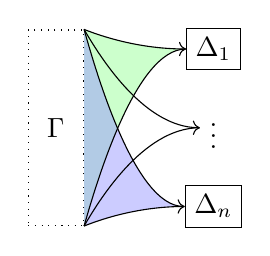
\begin{tikzpicture}[baseline]
    \path
    (-1,1) node (Gtop) {}
    (-1,0) node (G) {$\Gamma$}
    (-1,-1) node (Gbot) {}
    ;
    \node[draw,dotted,fit=(Gtop) (G) (Gbot)] (GG) {};

    \path
    (1,1) node[draw] (Dtop) {$\Delta_1$}
    (1,0) node (D) {$\vdots$}
    (1,-1) node[draw] (Dbot) {$\Delta_n$}
    ;

    \fill[green!20!white,opacity=1] (GG.north east)
    parabola[bend at end] (Dtop.west)
    parabola[bend at start] (GG.south east)
    -- cycle;
    \fill[blue!40!white,opacity=.5] (GG.north east)
    parabola[bend at end] (Dbot.west)
    parabola[bend at start] (GG.south east)
    -- cycle;

    \draw[->] (GG.north east) parabola[bend at end] (Dtop.west);
    \draw (GG.south east) parabola[bend at end] (Dtop.west);
    \draw[->] (GG.north east) parabola[bend at end] (D.west);
    \draw (GG.south east) parabola[bend at end] (D.west);
    \draw[->] (GG.north east) parabola[bend at end] (Dbot.west);
    \draw (GG.south east) parabola[bend at end] (Dbot.west);
  \end{tikzpicture}
\end{displaymath}

To see how this definition works, let us construct an example substitution:
$A, B \to C, B \Longrightarrow B, C$.
Because the codomain is a Cartesian product, it suffices to give two separate
substitutions, $A, B \to C, B \Longrightarrow B$ and
$A, B \to C, B \Longrightarrow C$, with a substitution into a singleton
context being just a term.
We indeed have terms $x : A, y : B \to C, z : B \vdash y : B$ and
$x : A, y : B \to C, z : B \vdash y\,z : C$.
It is also instructive to look at an identity substitution (which is also a
renaming), $A, B \Longrightarrow A, B$, witnessed by terms
$x : A, y : B \vdash x : A$ and $x : A, y : B \vdash y : B$.

When working with our semiring-annotated calculus \name{}, contexts are no
longer understood as Cartesian products.
This means that substitutions of type $\Gamma \Longrightarrow \Delta$ are no
longer equivalent to collections of substitutions
$\Gamma \Longrightarrow \Delta_i$.
Indeed, notice that we should still have an identity substitution of type
$\gr1A, \gr1B \Longrightarrow \gr1A, \gr1B$, but we do not have terms proving
either $\gr1A, \gr1B \vdash A$ or $\gr1A, \gr1B \vdash B$.
What we do have are terms $x : \gr1A, y : \gr0B \vdash x : A$ and
$x : \gr0A, y : \gr1B \vdash y : B$, and if we pointwise add together the
annotations of the two terms, we get back the original context
$x : \gr1A, y : \gr1B$.
Furthermore, adding up the annotations is not just a random operation;
linear contexts are understood to be tensor products of their elements, and
introduction rule for the tensor product involves summing the annotations of
the two sides.

For any annotated context $\Delta$, we have
$\Delta \vdash \bigotimes_{(\gr rx : A) \in \Delta}\oc\gr rA$ by iterated
application of $\otimes$-I with $\oc$-I and Var at the leaves.
Let $\Gamma = \grP\gamma$ and $\Delta = \grQ\delta$.
If we are to produce substitutions from $\Gamma$ to $\Delta$ in this
pattern, we simulate the applications of $\otimes$-I by producing, for each
element in $\Delta$, a usage context for $\gamma$ such that the whole collection
sums to $\grP$, then simulate the applications of $\oc$-I by dividing each of
the new usage contexts by the corresponding annotation in $\Delta$, calling
the divided usage contexts $\gr\Psi_x$, and finally, instead of a variable
from $\delta$, we give a term of type $\gr\Psi_x\gamma \vdash \delta_x$.
In summary, the constraint on the collection of usage contexts $\gr\Psi$ is
that $\grP = \sum_{(\gr rx : A) \in \Delta}\gr r\gr\Psi_x$.
Moreover, if we take $\grP$ and $\grQ$ to be row vectors and $\gr\Psi$ to be a
matrix, the latter expression is equal to the vector-matrix multiplication
$\grQ\gr\Psi$.
The resulting definition of simultaneous substitution is depicted below.

\begin{displaymath}
  \begin{tikzpicture}[baseline]
    \path
    (-1,1) node (Gtop) {}
    (-1,0) node (G) {$\grP\gamma$}
    (-1,-1) node (Gbot) {}
    ;
    \node[draw,dotted,fit=(Gtop) (G) (Gbot)] (GG) {};

    \path
    (1,1) node (Dtop) {}
    (1,0) node (D) {$\grQ\delta$}
    (1,-1) node (Dbot) {}
    ;
    \node[draw,dotted,fit=(Dtop) (D) (Dbot)] (DD) {};

    \draw[->,double] (GG) -- (DD);
  \end{tikzpicture}
  \coloneqq
  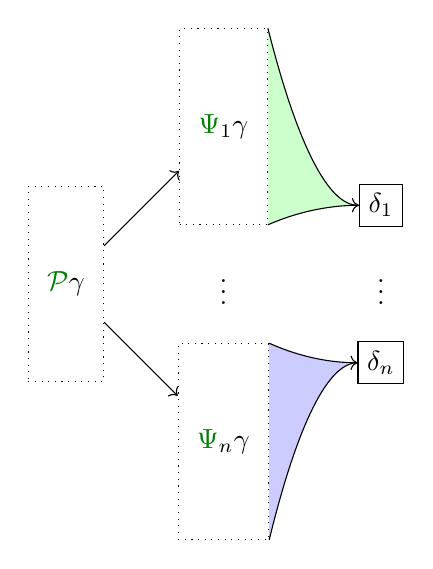
\begin{tikzpicture}[baseline]
    \path
    (-1,1) node (Gtop) {}
    (-1,0) node (G) {$\grP\gamma$}
    (-1,-1) node (Gbot) {}
    ;
    \node[draw,dotted,fit=(Gtop) (G) (Gbot)] (GG) {};

    \path
    (1,3) node (G1top) {}
    (1,2) node (G1) {$\gr\Psi_1\gamma$}
    (1,1) node (G1bot) {}
    ;
    \node[draw,dotted,fit=(G1top) (G1) (G1bot)] (GG1) {};
    \draw[->] (GG) -- (GG1);

    \path (1,0) node {$\vdots$};

    \path
    (1,-1) node (Gntop) {}
    (1,-2) node (Gn) {$\gr\Psi_n\gamma$}
    (1,-3) node (Gnbot) {}
    ;
    \node[draw,dotted,fit=(Gntop) (Gn) (Gnbot)] (GGn) {};
    \draw[->] (GG) -- (GGn);

    \path
    (3,1) node[draw] (Dtop) {$\delta_1$}
    (3,0) node (D) {$\vdots$}
    (3,-1) node[draw] (Dbot) {$\delta_n$}
    ;

    \fill[green!20!white] (GG1.north east)
    parabola[bend at end] (Dtop.west)
    parabola[bend at start] (GG1.south east)
    -- cycle;
    \draw[->] (GG1.north east) parabola[bend at end] (Dtop.west);
    \draw (GG1.south east) parabola[bend at end] (Dtop.west);

    \fill[blue!20!white] (GGn.north east)
    parabola[bend at end] (Dbot.west)
    parabola[bend at start] (GGn.south east)
    -- cycle;
    \draw[->] (GGn.north east) parabola[bend at end] (Dbot.west);
    \draw (GGn.south east) parabola[bend at end] (Dbot.west);
  \end{tikzpicture}
  \quad\textrm{where }\grP = \grQ\gr\Psi
\end{displaymath}

In type theory, we write out the definition as follows.

\begin{displaymath}
  \sum_{\gr\Psi : \size\Delta \to \size\Gamma \to \Ann}
    \left(\grP = \grQ\gr\Psi\right) \times
    \prod_{(x : A) \in \delta}\gr\Psi_x\gamma \vdash A
\end{displaymath}

We can see the step-by-step construction of a substitution play out by adapting
the previous example to have type
$\gr0A, \gr2(B \multimap C), \gr3B \Longrightarrow \gr1B, \gr2C$.
To split the goal up, we note that $
\begin{pmatrix} \gr0 & \gr2 & \gr3 \end{pmatrix} =
\begin{pmatrix} \gr0 & \gr0 & \gr1 \end{pmatrix} +
\begin{pmatrix} \gr0 & \gr2 & \gr2 \end{pmatrix}
$, so it suffices to give substitutions of types
$\gr0A, \gr0(B \multimap C), \gr1B \Longrightarrow \gr1B$ and
$\gr0A, \gr2(B \multimap C), \gr2B \Longrightarrow \gr2C$.
Furthermore, our term calculus only supports $\gr1$-annotated conclusions,
so we divide the second substitution type through by $\gr2$.
Finally, we give the terms largely as before:
$\gr0x : A, \gr0y : B \to C, \gr1z : B \vdash y : B$ and
$\gr0x : A, \gr1y : B \to C, \gr1z : B \vdash z\,y : C$.

While we naturally derive a matrix as a fragmentation of a usage vector, we can
get a slightly cleaner presentation by instead using an abstract linear map.
Let $\gr\Psi$ now be a linear map of type
$\Ann^{\size\Delta} \to \Ann^{\size\Gamma}$, with application written postfix.
The equation $\grP = \grQ\gr\Psi$ remains unchanged.
Where we previously wrote $\gr\Psi_x$, the most direct replacement would be
$\langle x \rvert\gr\Psi$, with $\langle x \rvert$ being the $x$th basis row
vector.
But then we notice that $\langle x \rvert$ is exactly the $\grQprime$ satisfying
$\grQprime\delta \sqni x : B$.
This gives us the following definition, which can be verified by equationally
substituting $\grPprime$ and expanding the definition of $\sqni$.

\begin{displaymath}
  \sum_{\gr\Psi : \Ann^{\size\Delta} \to \Ann^{\size\Gamma}}
    \left(\grP = \grQ\gr\Psi\right) \times
    \prod_{A,\grQprime,\grPprime} \left(
    \grPprime = \grQprime\gr\Psi \to \grQprime\delta \sqni A \to
    \grPprime\gamma \vdash A\right)
\end{displaymath}

We now have a new reading for the interpretation of a linear substitution:
a linear map $\gr\Psi$ relating the two usage vectors $\grP$ and $\grQ$, and
for any two similarly related usage vectors $\grPprime$ and $\grQprime$, we
have a type-preserving function from variables in $\grQprime\delta$ to terms in
$\grPprime\gamma$.
Even though we don't use $\gr\Psi$ as a matrix containing fragmented usage
vectors, we can still justify why it should be a \emph{linear} map.
We need $\gr\Phi$ to respect all fragmentation of the usage context in a typing
rule, and we know that all such fragmentation is done by linear operations
zero, addition, and scaling by a constant.
\todo{Expand. Substitutions need to preserve everything done to the context,
and linear things are all we do to the context.}

Taking a lead from \cref{sec:kits}, we deduce a definition of
\emph{environment} by replacing the $\vdash$ in the definition of simultaneous
substitution by an arbitrary type family $\mathcal V$.
Letting $\mathcal V$ be $\sqni$ gives us a notion of simultaneous renaming,
allowing for renamings with types such as
$\gr6A, \gr0B, \gr1C \stackrel\sqni\Longrightarrow \gr1C, \gr2A, \gr4A$.

It is worth noting that, when contexts are Cartesian products, passing from
``a map into $\Delta$'' to ``for each $A \in \Delta$, a map into $A$'' does not
lose any generality because the universal property of Cartesian products
states that every map into a Cartesian product can be given factor-wise.
Hence, $\Delta$ and the one-element context $\prod_{A \in \Delta}A$ are
isomorphic in the category of contexts and simultaneous substitution.
However, tensor products are not limits, so don't have the same universal
property.
Indeed, many annotated contexts are not isomorphic to the weighted product of
their elements.
For example, we do not have a substitution of type
$\gr1(A \otimes B) \Longrightarrow \gr1A, \gr1B$ because we would first need
to pattern-match on the tensor product \emph{before} trying to derive the
target context.
This loss of generality is however justified when we consider the action of a
substitution.
Substitutions should only be replacing variables by terms, whereas if
substitutions were allowed to pattern-match before introducing the target, then
the substitution would have to replace the original term by a term that first
pattern-matches and then continues like the original term.

\section{Properties of linear environments}\label{sec:lenv}
\begin{remark}
  Given an environment $\rho : \grP\gamma \env\V \grQ\delta$ and a $\grPprime$
  and a $\grQprime$ such that $\grPprime = \grQprime\plr{\rho.\gr\Psi}$,
  there is also an environment of type $\grPprime\gamma \env\V \grQprime\delta$
  with the same linear map and action on variables.
\end{remark}
\begin{proof}
  The only part of the definition of an environment dependent on $\grP$ or
  $\grQ$ is the constraint $\grP = \grQ\gr\Psi$, which we are able to replace
  for $\grPprime$ and $\grQprime$.
\end{proof}

When constructing an environment, we can do so by cases on the shape of the
target context.
We can create an environment into the empty context when all usage annotations
on the source context are $\gr0$.
We can create an environment into a concatenated context when we can additively
split up the annotations of the source context and produce environments into
both halves from the split sources.
We can create an environment into a singleton context when there is a context
$\gr r$ times smaller than the source context in which we can produce a value
of the appropriate type.

\begin{lemma}\label{thm:construct-env}
  We can define all of the following equivalences for any values of the free
  variables.
  \begin{itemize}
    \item $\forallb{I \dotlr \plr{{-} \env\V {\cdot}}}$
    \item $\forallb{\plr{{-} \env\V \Gamma} \sep \plr{{-} \env\V \Delta}
      \dotlr \plr{{-} \env\V \Gamma, \Delta}}$
    \item
      $\forallb{\gr r \cdot \plr{\V\,(-)\,A} \dotlr \plr{{-} \env\V \gr rA}}$
  \end{itemize}
\end{lemma}
\begin{proof}
  There are 6 cases to check.
  Throughout, we write $\Gamma$ as $\grP\gamma$ and $\Delta$ as $\grQ\delta$
  when convenient.
  \begin{description}
    \item[$I(\to)$]
      Let $\gr\Psi$ be the unique linear map out of the zero space.
      By definition, $\gr0 = \grQ\gr\Psi$.
      There are no variables to act upon.
    \item[$I(\gets)$]
      $\grQ\gr\Psi$ is an empty sum, so if $\grP = \grQ\gr\Psi$ then
      $\grP = \gr0$.
    \item[$\sep(\to)$]
      Let the given environments be $\rho : \grRl\theta \env\V \Gamma$ and
      $\sigma : \grRr\theta \env\V \Delta$, with $\grR = \grRl + \grRr$.
      Define $\gr\Psi \coloneqq [\rho.\gr\Psi, \sigma.\gr\Psi]$, using the
      coproduct structure of the concatenated vector space.
      We have $\grR = \grRl + \grRr =
      \grP\plr{\rho.\gr\Psi} + \grQ\plr{\sigma.\gr\Psi} =
      \plr{\grP, \grQ}\gr\Psi$.
      To act on variables, we are given
      $\grRprime = \plr{\grPprime, \grQprime}\gr\Psi$ and
      $\grPprime\gamma, \grQprime\delta \sqni A$.
      Without loss of generality, let us have $\grPprime\gamma \sqni A$ and
      $\grQprime = \gr0$.
      Thus, $\grRprime = \grPprime\plr{\rho.\gr\Psi}$, and we can act on the
      variable using $\rho$.
    \item[$\sep(\gets)$]
      Let the unnamed context be $\Theta$, also written $\grR\theta$.
      The linear map
      $\gr\Psi : \Ann^{\size\Gamma + \size\Delta} \to \Ann^{\size\Theta}$ splits
      into
      $\gr\Psi_{\gr l} : \Ann^{\size\Gamma} \to \Ann^{\size\Theta}
      \coloneqq \langle \id, 0 \rangle; \gr\Psi$ and
      $\gr\Psi_{\gr r} : \Ann^{\size\Delta} \to \Ann^{\size\Theta}
      \coloneqq \langle 0, \id \rangle; \gr\Psi$, using the product structure of
      the concatenated vector space.
      Let $\grRl \coloneqq \grP\gr\Psi_{\gr l}$ and
      $\grRr \coloneqq \grQ\gr\Psi_{\gr r}$, by definition satisfying the
      required equations.
      For the action on variables, let us consider the left environment.
      We are given $\grRprime = \grPprime\gr\Psi_{\gr l}$ and
      $\grPprime\gamma \sqni A$.
      From these, we get
      $\grRprime = \grPprime\gr\Psi_{\gr l} = \plr{\grPprime, \gr0}\gr\Psi$ and
      $\grPprime\gamma, \gr0\delta \sqni A$.
      We can therefore act using the original environment.
    \item[$\cdot(\to)$]
      Let $\grP$ and $\grPprime$ be such that $\grP = \gr r\grPprime$ and let
      $v : \V\,\grPprime\gamma\,A$.
      Let $\gr\Psi : \Ann \to \Ann^{\size\gamma}
      \coloneqq \gr r\gr' \mapsto \gr r\gr'\grPprime$.
      By definition and the previous assumption, we have $\grP = \gr r\gr\Psi$.
      When acting on a variable, we have $\grP\gr{''} = \gr r\gr'\gr\Psi$
      and $\gr r\gr'A \sqni A'$.
      The latter tells us that $A = A'$ and $\gr r\gr' = \gr1$.
      Thus, $\grP\gr{''} = \grPprime$.
      We therefore need a value of type $\V\,\grPprime\gamma\,A$, which we can
      take to be $v$.
    \item[$\cdot(\gets)$]
      Let us have an environment of type $\grP\gamma \env\V \gr rA$.
      We want to use its action on variables to yield a value.
      To do this, we let $\grPprime \coloneqq \gr1\gr\Psi$, and use this
      equation, together with the fact that we have a variable of type
      $\gr1A \sqni A$, to get a value of type $\V\,\grPprime\gamma\,A$.
      Furthermore, we derive $\grP = \gr r\gr\Psi = \gr r\grPprime$, as
      required.
  \end{description}
\end{proof}

We could, indeed, use these three clauses to define what an environment is.
However, I find them difficult to work with, as it is often easier to do
linear algebraic proofs separately from the rest of an environment.
For identity and composition, as we are about to see, the original definition
is easier to use because we can rely on the identity and composition of linear
maps.
Concretely, an inductive proof of identity would, for example, involve
constructing an environment of type
$\grP\gamma, \grQ\delta \env\V \grP\gamma, \grQ\delta$ by constructing
environments of types $\grP\gamma, \gr0\delta \env\V \grP\gamma$ and
$\gr0\gamma, \grQ\delta \env\V \grQ\delta$.
These are not identity environments, so we would have to strengthen the
induction hypothesis.

One of the primary test cases for environments is simultaneous substitution,
which will look like the following rule.
The admissibility of substitution will be by induction on the derivation of
$\Delta \vdash A$, so we will need to be able to adapt any environment we are
given to work with any possible context of new premises.
In the simply typed case, the only change to the context we encountered was the
binding of new variables.
Now, with usage annotations, we furthermore have linear decompositions of the
context, necessitating changes to the environment whenever usage annotations
change.
I will deal first with linear decompositions.

\begin{displaymath}
  \begin{prooftree}
    \hypo{\Gamma \env{\vdash} \Delta}
    \hypo{\Delta \vdash A}
    \infer2[sub]{\Gamma \vdash A}
  \end{prooftree}
\end{displaymath}

There are three kinds of linear decompositions we have to deal with: zero,
addition, and scaling; corresponding to bunched connectives $I^*$, $\sep$, and
$\gr r \cdot {}$, respectively.
In each case, we have a simple preservation lemma, transforming an environment
of type $\Gamma \env\V \Delta$ and a decomposition of $\Delta$ into a
decomposition of $\Gamma$ and environments for all of the decomposed fragments
of $\Gamma$ and $\Delta$.

\begin{lemma}[environments preserve zero]\label{thm:lr-env-zero}
  Given an environment of type $\grP\gamma \env\V \grQ\delta$ such that
  $\grQ \leq \gr 0$, we also have that $\grP \leq \gr 0$.
\end{lemma}
\begin{proof}
  $\grP \leq \grQ\gr\Psi \leq \gr0\gr\Psi = \gr0$, by environment
  compatibility and monotonicity and linearity of $\gr\Psi$.
\end{proof}

\begin{lemma}[environments preserve addition]\label{thm:lr-env-add}
  Given an environment of type $\grP\gamma \env\V \grQ\delta$ such that
  $\grQ \leq \grQl + \grQr$ for some $\grQl$ and $\grQr$, we also have $\grPl$
  and $\grPr$ such that $\grP \leq \grPl + \grPr$ and there are environments
  of types $\grPl\gamma \env\V \grQl\delta$ and
  $\grPr\gamma \env\V \grQr\delta$.
\end{lemma}
\begin{proof}
  Let $\grPl \coloneqq \grQl\gr\Psi$ and $\grPr \coloneqq \grQr\gr\Psi$.
  Then, $\grP \leq \grQ\gr\Psi \leq \plr{\grQl + \grQr}\gr\Psi =
  \grQl\gr\Psi + \grQr\gr\Psi = \grPl + \grPr$, satisfying the first condition.
  Because clearly $\grPl \leq \grQl\gr\Psi$ and $\grPr \leq \grQr\gr\Psi$,
  \cref{thm:env-resize} on the original environment gives us the required
  pair of new environments.
\end{proof}

\begin{lemma}[environments preserve scaling]\label{thm:lr-env-scale}
  Given an environment of type $\grP\gamma \env\V \grQ\delta$ such that
  $\grQ \leq \gr r\grQprime$ for some $\grQprime$, we also have a $\grPprime$
  such that $\grP \leq \gr r\grPprime$ and there is an environment of type
  $\grPprime\gamma \env\V \grQprime\delta$.
\end{lemma}
\begin{proof}
  Let $\grPprime \coloneqq \grQprime\gr\Psi$.
  Then, $\grP \leq \grQ\gr\Psi \leq \plr{\gr r\grQprime}\gr\Psi =
  \gr r\plr{\grQprime\gr\Psi} = \gr r\grPprime$, satisfying the first condition.
  Because clearly $\grPprime \leq \grQprime\gr\Psi$,
  \cref{thm:env-resize} on the original environment gives us the required
  new environment.
\end{proof}

Finally, I will also take the opportunity to give the bind lemma, allowing
environments to incorporate newly bound variables.
In the intuitionistic case, the bind lemma had two requirements on $\V$: $\V$
admits weakening and we can map variables into $\V$-values.
With usage annotations, the former is unreasonable, but it turns out that we
only need weakening by variables whose usage annotation is less than or equal
to $\gr0$.
The latter stays as-is, with the note that ``variable'' now means a
usage-checked variable.

\begin{lemma}[bind]\label{thm:lr-bind}
  Given functions
  ${\swarrow^k} : \forall \Gamma, \grR, \theta.~\grR \leq \gr0 \to
  \forallb{\V\,\Gamma \dotto \V\,\plr{\Gamma, \grR\theta}}$ and
  $\mathrm{vr} : \forallb{{\sqni} \dotto \V}$, we can turn an environment of
  type $\Gamma \env\V \Delta$ into an environment of type
  $\Gamma, \Theta \env\V \Delta, \Theta$ for any context $\Theta$.
\end{lemma}
\begin{proof}
  Let $\grP\gamma \coloneqq \Gamma$, $\grQ\delta \coloneqq \Delta$, and
  $\grR\theta \coloneqq \Theta$.
  Let the new linear map $\gr\Psi\gr' : \Ann^{\size\Delta + \size\Theta} \to
  \Ann^{\size\Gamma + \size\Theta}$ be $\gr\Psi \oplus \gr I$.
  That is, in block matrix notation,
  $\begin{pmatrix} \gr\Psi & \gr0 \\ \gr0 & \gr I \end{pmatrix}$.
  Checking that this linear map fits, we have
  $\begin{pmatrix}\grP & \grR\end{pmatrix}
  \leq \begin{pmatrix}\grQ\gr\Psi & \grR\gr I\end{pmatrix}
  = \begin{pmatrix}\grQ & \grR\end{pmatrix}\plr{\gr\Psi \oplus \gr I}$.
  For the action on variables, we are given vectors $\grPprime$,
  $\grR\gr'_\grP$, $\grQprime$, and $\grR\gr'_\grQ$ such that
  $\begin{pmatrix} \grPprime & \grR\gr'_\grP \end{pmatrix} \leq
  \begin{pmatrix} \grQprime & \grR\gr'_\grQ \end{pmatrix}
  \plr{\gr\Psi \oplus \gr I}$ and we have a variable of type
  $\grQprime\delta, \grR\gr'_\grQ\theta \sqni A$ for some type $A$.
  The constraint on the new vectors reduces to $\grPprime \leq \grQprime\gr\Psi$
  and $\grR\gr'_\grP \leq \grR\gr'_\grQ$.
  From the variable we either have a variable $x$ in $\delta$ with
  $\grQprime \leq \langle x \rvert$ and $\grR\gr'_\grQ \leq \gr0$, or a
  variable $y$ in $\theta$ with $\grQprime \leq \gr0$ and
  $\grR\gr'_\grQ \leq \langle y \rvert$.
  In the former case, the action of the original environment on $x$ gives us a
  $\V$-value in $\grPprime\gamma$, and the $\gr0$-weakening principle
  $\swarrow^k$, noting that $\grR\gr'_\grP \leq \grR\gr'_\grQ \leq \gr0$, gives
  us a $\V$-value in $\grPprime\gamma, \grR\gr'_\grP\theta$.
  In the latter case, we have that
  $\begin{pmatrix} \grPprime & \grR\gr'_\grP \end{pmatrix}
  \leq \begin{pmatrix} \grQprime\gr\Psi & \grR\gr'_\grQ \end{pmatrix}
  \leq \begin{pmatrix} \gr0\gr\Psi & \langle y \rvert \end{pmatrix}
  = \begin{pmatrix} \gr0 & \langle y \rvert \end{pmatrix}
  = \left\langle {\searrow}y \right\rvert$, so $y$ also serves as a
  usage-checked variable in $\grPprime\gamma, \grR\gr'_\grP\theta$.
  From this usage-checked variable, we get a $\V$-value in the same context
  using $\mathrm{vr}$.
\end{proof}

The requirements for identity and composition of environments look a bit like
the unit and lift of a Kleisli triple.

\begin{lemma}[Identity environment]
  Given a function $\mathrm{vr} : \forallb{{\sqni} \dotto \V}$, for any
  $\Gamma$ we have an environment of type $\Gamma \env\V \Gamma$.
\end{lemma}
\begin{proof}
  Let $\gr\Psi$ be the identity map, which clearly satisfies
  $\grP = \grP\gr\Psi$.
  When acting on a variable, the equation $\grPprime = \grQprime\gr\Psi$ means
  that $\grPprime = \grQprime$, so we want, from a variable of type
  $\grPprime\gamma \sqni A$, a value of type $\V\,\grPprime\gamma\,A$, which
  we can get from $\mathrm{vr}$.
\end{proof}

\begin{lemma}\label{thm:env-comp-lemma}
  Given an environment $\rho : \Gamma \env\U \Delta$ for which we have, for any
  $\grPprime$ and $\grQprime$ such that
  $\grPprime = \grQprime\plr{\rho.\gr\Psi}$, we have a function
  $\mathrm{lift}_\rho :
  \forallb{\V\,\grQprime\delta \dotto \W\,\grPprime\gamma}$,
  we can map environments of type $\Delta \env\V \Theta$ into environments of
  type $\Gamma \env\W \Theta$.
\end{lemma}
\begin{proof}
  Let $\rho$ be as in the statement, and let $\sigma : \Delta \env\V \Theta$.
  For the environment we are constructing, let
  $\gr\Psi \coloneqq \sigma.\gr\Psi; \rho.\gr\Psi$, noting that
  $\grP = \grQ\plr{\rho.\gr\Psi} =
  \plr{\grR\plr{\sigma.\gr\Psi}}\plr{\rho.\gr\Psi}$.
  For the action on variables, we are given $\grPprime = \grRprime\gr\Psi$ with
  $\grRprime\theta \sqni A$.
  We can immediately apply the action of $\sigma$, giving us a value of type
  $\V\,\plr{\grRprime\plr{\sigma.\gr\Psi}}\,A$.
  We note that
  $\grPprime = \plr{\grRprime\plr{\sigma.\gr\Psi}}\plr{\rho.\gr\Psi}$, and
  apply $\mathrm{lift}_\rho$ to get the desired value.
\end{proof}

\begin{corollary}[Composition of environments]
  Given a function
  $\mathrm{lift} : \plr{\rho : \grP\gamma \env\U \grQ\delta} \to
  \forall \grPprime, \grQprime.~\grPprime = \grQprime\plr{\rho.\gr\Psi} \to
  \forallb{\V\,\grQprime\delta \dotto \W\,\grPprime\gamma}$, then we can
  compose environments of types $\Gamma \env\U \Delta$ and
  $\Delta \env\V \Theta$ into an environment of type $\Gamma \env\W \Theta$.
\end{corollary}

\begin{example}
  We can derive the following instances of environment composition.
  \begin{itemize}
    \item If $\U = \V = \W = {\sqni}$, then $\mathrm{lift}$ is given by the
      action of the renaming $\rho$ on variables.
      This allows us to derive composition of renamings.
    \item More generally, if $\V = {\sqni}$ and $\U = \W$, we can still use
      the action of the environment $\rho$.
      This means that renamings post-compose with any other sort of environment.
    \item If $\V = \W = {\vdash}$, then $\mathrm{lift}$ is given by a
      syntactic traversal.
      For example, if $\U = {\sqni}$, we need the action of renaming on terms
      to show that a renaming followed by a substitution composes to a
      substitution.
      If $\U = {\vdash}$, then the action of substitution on terms gives us that
      substitutions compose.
    \item More generally, if $\V = {\vdash}$ and we have a semantics from
      $\U$ to $\W$, then $\mathrm{lift}$ can be given by the semantic traversal
      of terms.
  \end{itemize}
\end{example}

% Concatenation is difficult; save to after I've talked about renamings.

% Finally for this section, we give the conditions under which the
% context-forming operations (empty, concatenation, and singleton) have a
% functorial action with respect to $\V$-environments.
%
% \begin{lemma}
%   For any $\V$, there is an environment ${\cdot} \env\V {\cdot}$.
% \end{lemma}
% \begin{proof}
%   By \autoref{thm:construct-env}, it suffices to show $I\,{\cdot}$, which is
%   trivially true.
% \end{proof}

\section{Substitution is admissible in \name{}}\label{sec:lrsub}
\def\LRKits{../agda/processed-latex/LRKits.tex}

I can now show that, using the notion of \emph{environment} derived in
\cref{sec:lrkits}, we can replicate the Agda proofs from
\cref{sec:syntactic-kits} in the usage-aware setting of $\name$.
From \cref{sec:lenv}, we know that environments are preserved under all
syntax-forming operations: zero, addition, scaling, and binding.
What is left is to show how these properties are deployed, and also how to
go on and prove the admissibility of simultaneous renaming, simultaneous
substitution, and then single substitution.

There are a few notational changes necessary in the Agda code, compared to the
typeset mathematics above.
Usage vectors, elsewhere called $\grP$, $\grQ$, and $\grR$ are rendered as
\AgdaBound{P}, \AgdaBound{Q}, and \AgdaBound{R}, respectively.
Usage contexts and typing contexts are tied together with the
\AgdaInductiveConstructor{ctx} constructor, rather than simple juxtaposition.
Environments, elsewhere notated $\Gamma \env\V \Delta$, are rendered as
\AgdaRecord{[}\AgdaSpace{}\AgdaBound{$\V$}\AgdaSpace{}\AgdaRecord{]}%
\AgdaSpace{}\AgdaBound{$\Gamma$}\AgdaSpace{}\AgdaRecord{$\Rightarrow^e$}%
\AgdaSpace{}\AgdaBound{$\Delta$}.

We start with a slightly modified definition of \AgdaRecord{Kit}.
We saw in \cref{thm:lr-bind} that in the usage-annotated context, we restrict
weakening of $\V$-values to just $\gr0$-use variables.
Meanwhile, the function $\mathrm{vr}$, also seen in \cref{thm:lr-bind}, maps
usage-checked variables to $\V$-values, and the function $\mathrm{tm}$, used
to coerce $V$-values yielded by the environment into terms, stays the same.
I state weakening in a slightly different way than previously, so as to help
unification against a known result type (avoiding the problem described by
\citet{McBride12} as \emph{green slime}).
The type \AgdaFunction{Weakening}\AgdaSpace{}\AgdaBound{$\V$} can be read as
saying that, for any context $\grP\gamma$ of shape $s + t$, if the right of
$\grP$ is below $\gr0$, then a value in the left part of $\grP\gamma$ weakens
to a value in the whole of $\grP\gamma$.

\ExecuteMetaData[\LRKits]{Kit}

To demonstrate the important points succinctly, I cut \name{} down to just the
$\oc\gr r$-fragment.
The introduction rule and pattern-matching eliminator feature scaling, addition,
and variable binding, missing out only on sharing (which is trivial) and zero
(which is simpler than, and analogous to, addition).
The resulting type of well typed terms is below.

\ExecuteMetaData[\LRKits]{Tm}

Given a \AgdaRecord{Kit}, \cref{thm:lr-bind} looks like the following.
The \AgdaField{lookup} clauses still contain essentially the same structure as
in the intuitionistic case: discriminating on whether the variable is old or
new, using the given environment \AgdaBound{$\rho$} and weakening on the old
variables, and using \AgdaField{vr} to repackage new variables.
I will not explain any of the algebraic manipulations here; see
\cref{thm:lr-bind}.

\ExecuteMetaData[\LRKits]{bindEnv}

Given \AgdaFunction{bindEnv} (\cref{thm:lr-bind}), \AgdaFunction{env-+}
(\cref{thm:lr-env-add}), and \AgdaFunction{env-*} (\cref{thm:lr-env-scale}),
we can reproduce the syntactic traversal \AgdaFunction{trav}.
With all these lemmas in place, writing \AgdaFunction{trav}
becomes routine.
When processing a rule, we work our way up through the
premise connectives, applying \AgdaFunction{env-*} wherever we see a
\AgdaFunction{$\cdot^c$}, \AgdaFunction{env-+} wherever we see a
\AgdaFunction{$*^c$}, and \AgdaFunction{bindEnv} wherever we see a
\AgdaFunction{Bind}.
We then use whatever environments (with names beginning with
\AgdaBound{$\rho$}) and whatever usage vector splitting facts (with names
beginning with \AgdaBound{sp}) come out of this process to recursively
traverse the subterms and recombine the results.

\ExecuteMetaData[\LRKits]{trav}

Instantiating the generic syntactic traversal \AgdaFunction{trav} to renaming
looks just like it did in the intuitionistic case.
I have consistently replaced intuitionistic variables by linear variables, so
\AgdaFunction{id} and \AgdaInductiveConstructor{var} still work to embed
variables into variables and terms, respectively.
Weakening for variables \AgdaFunction{$\swarrow^v$} (not pictured) has been
updated to note that, for $\grP \leq \bra x$ and $\grR \leq \gr0$, we also have
$\begin{pmatrix} \grP & \grR \end{pmatrix} \leq \bra{{\swarrow}x}$.

\ExecuteMetaData[\LRKits]{var-kit}

In the intuitionistic case, environments were just functions, so we passed the
variable weakening function \AgdaFunction{$\swarrow^v$} to the function
\AgdaFunction{ren} to yield a term weakening function.
However, a usage-aware environment is a function packed together with usage
distribution data.
As such, we must make an environment version of \AgdaFunction{$\swarrow^v$}.
I start with a general lemma \AgdaFunction{$\swarrow$\^{}Env}, stating that if
$\V$ supports weakening, then so do $\V$-environments (in their domain
context).
This lemma then specialises to variables, with the identity renaming
\AgdaFunction{id\^{}Env} on the left part of the context and the proof
\AgdaBound{R0} that the right part of the context is below $\gr0$ combining
to give the desired weakening environment.

\ExecuteMetaData[\LRKits]{dlv-env}

This is what we need to instantiate \AgdaFunction{trav} for substitution.
As a reminder, I also give the type of \AgdaFunction{sub} in rule form.

\ExecuteMetaData[\LRKits]{sub}
\[
  \ebrule{%
    \hypo{\Gamma \env\vdash \Delta}
    \hypo{\Delta \vdash B}
    \infer2[sub]{\Gamma \vdash B}
  }
\]

Finally, the simultaneous substitution \AgdaFunction{sub} specialises to
single substitution \AgdaFunction{sub[-]}.
Single substitution is stated as an admissible rule below.
To substitute in for $\gr r$-many $A$ in the second term, we need to derive
one $A$ with usages $\grP$, and then assert that the result can handle the
usages of the original term $\grQ$, plus $\gr r$-many copies of $\grP$.

\[
  \ebrule{%
    \hypo{\grR \leq \grQ + \gr r\grP}
    \hypo{\grP\gamma \vdash A}
    \hypo{\grQ\gamma, \gr rA \vdash B}
    \infer3[singleSub]{\grR\gamma \vdash B}
  }
\]

The proof strategy for producing the substitution \AgdaFunction{$\sigma$} is
to proceed structurally on the codomain context $\grQ\gamma, \gr rA$ using
\cref{thm:construct-env}, applying the identity substitution
\AgdaFunction{id\^{}Env} on the $\gamma$ half, and dropping the term
\AgdaBound{t} in place of the variable we are substituting for.

\ExecuteMetaData[\LRKits]{subSingle}

\section{Recursion}\label{sec:rec}
Based on an intuitive understanding of ``usage'', recursion introduces a new
phenomenon relative to the forms of programs we have seen so far:
terms can be used an unbounded number of times.
For example, notice the following reduction in Agda.

\missingfigure{\texttt{foldr \_+\_ 0 (1 :: 2 :: 3 :: []) = 1 + (2 + (3 + 0))}}

The function \AgdaFunction{\_+\_} has been copied into 3 different places in
the running of the program.
This copying is despite no type telling us that \AgdaFunction{\_+\_} would be
used 3 times (both \verb|[1,2,3]| and \verb|[2,3]| have type
\AgdaDatatype{List}\AgdaSpace{}\AgdaDatatype{$\mathbb N$}, despite the
corresponding folds using \AgdaFunction{\_+\_} a different number of times).
As such, when checking an application of \AgdaFunction{foldr}, we need check
that we can use its functional argument (\AgdaFunction{\_+\_} in this case) an
arbitrary number of times.
If we were to fix $\Ann$ as the $\{\gr0, \gr1, \gr\omega\}$ posemiring, then
wrapping the type of the functional argument in $\oc\gr\omega$ would suffice.
However, we want to remain generic in the choice of semiring.

I propose the following additions to \name{} to support a broad class of
inductive types.
I define strictly positive functors syntactically, with the only notable
restriction being not being allowed to use the type variable $X$ in the domain
of a function type.
I then add least fixed points of such strictly positive functors to the syntax
of types.

\begin{align*}
  U &\Coloneqq A \multimap (-) \mid \oc\gr r(-) \\
  {\odot} &\Coloneqq {\otimes} \mid {\oplus} \mid {\with} \\
  F[X], G[X] &\Coloneqq X \mid A \mid U(F[X]) \mid F[X] \odot G[X] \\
  A &\Coloneqq \cdots \mid \mu X.~F[X]
\end{align*}

\begin{example}
  We may define $\mathrm{List}_A \coloneqq \mu X.~I \oplus \plr{A \otimes X}$.
\end{example}

In the typing rules, introduction of an inductive type is standard.
For the elimination rule, we follow a similar pattern to other pattern-matching
rules --- $\oplus$-E, $\otimes$-E, and $\oc$-E --- by splitting the context
and typing the eliminand in one half ($\grP$).
We type the continuation in the other half, but because the continuation may
be used multiple times, and in a modal context, we require that $\grQ$ is
preserved by all linear operations.

\begin{displaymath}
  \begin{prooftree}
    \hypo{\grR\gamma \vdash F[\mu X.~F[X]]}
    \infer1[$\mu$-I]{\grR\gamma \vdash \mu X.~F[X]}
  \end{prooftree}
\end{displaymath}
\begin{displaymath}
  \begin{prooftree}
    \hypo{\grR \leq \grP + \grQ}
    \hypo{\grP\gamma \vdash \mu X.~F[X]}
    \hypo{%
      \begin{matrix*}[l]
        \grQ \leq \gr0 \\
        \grQ \leq \grQ + \grQ \\
        \forall \gr r.~\grQ \leq \gr r\grQ
      \end{matrix*}%
    }
    \hypo{\grQ\gamma, \gr1F[C] \vdash C}
    \infer4[$\mu$-E]{\grR\gamma \vdash C}
  \end{prooftree}
\end{displaymath}

\begin{example}\label{thm:list-rules}
  For lists, we can derive the following introduction and elimination rules
  (with usage constraints omitted for brevity when obvious).

  \begin{align*}
    \begin{prooftree}
      \hypo{\grR \leq \gr0}
      \infer1[$I$-I]{I}
      \infer1[$\oplus$-I$_0$]%
      {\grR\gamma \vdash I \oplus \plr{A \otimes \mathrm{List}_A}}
      \infer1[$\mu$-I]{\grR\gamma \vdash \mathrm{List}_A}
    \end{prooftree}
    &&
    \begin{prooftree}
      \hypo{\grR \leq \grP + \grQ}
      \hypo{\grP\gamma \vdash A}
      \hypo{\grQ\gamma \vdash \mathrm{List}_A}
      \infer3[$\otimes$-I]{\grR\gamma \vdash A \otimes \mathrm{List}_A}
      \infer1[$\oplus$-I$_1$]%
      {\grR\gamma \vdash I \oplus \plr{A \otimes \mathrm{List}_A}}
      \infer1[$\mu$-I]{\grR\gamma \vdash \mathrm{List}_A}
    \end{prooftree}
  \end{align*}
  \begin{displaymath}
    \begin{prooftree}
      \hypo{\grP\gamma \vdash \mathrm{List}_A}
      \infer0[Var]{\gr0\gamma, \gr1\plr{I \oplus \plr{A \otimes C}}
        \vdash I \oplus \plr{A \otimes C}}
      \hypo{\nabla^n}
      \hypo{\nabla^c}
      \infer3[$\oplus$-E]{\grQ\gamma, \gr1\plr{I \oplus \plr{A \otimes C}}
        \vdash C}
      \infer2[$\mu$-E]{\grR\gamma \vdash C}
    \end{prooftree}
  \end{displaymath}
  \begin{align*}
    \textrm{where }\nabla^n &\coloneqq
    \begin{prooftree}
      \infer0[Var]{\gr0\gamma, \gr1I \vdash I}
      \hypo{\grQ\gamma \vdash C}
      \infer1[Wk]{\grQ\gamma, \gr0I \vdash C}
      \infer2[$I$-E]{\grQ\gamma, \gr1I \vdash C}
      \infer1[Wk]{\grQ\gamma, \gr0\plr{I \oplus \plr{A \otimes C}}, \gr1I
        \vdash C}
    \end{prooftree}
    \\\\
    \textrm{and }\nabla^c &\coloneqq
    \begin{prooftree}
      \infer0[Var]{\gr0\gamma, \gr1\plr{A \otimes C} \vdash A \otimes C}
      \hypo{\grQ\gamma, \gr1A, \gr1C \vdash C}
      \infer1[Wk]{\grQ\gamma, \gr0\plr{A \otimes C}, \gr1A, \gr1C \vdash C}
      \infer2[$\otimes$-E]{\grQ\gamma, \gr1\plr{A \otimes C} \vdash C}
      \infer1[Wk]%
      {\grQ\gamma, \gr0\plr{I \oplus \plr{A \otimes C}}, \gr1\plr{A \otimes C}
        \vdash C}
    \end{prooftree}
  \end{align*}
\end{example}

Following \cref{sec:lnd}, I want to turn the ad hoc constraints on $\grP$,
$\grQ$, and $\grR$ into the result of some premise combinators.
To do this, I introduce a new combinator $\Box^{0{+}{\times}}$ defined below,
along with the resulting implicit-context typing rules.

\begin{align*}
  \plr{\Box^{0{+}{\times}}\,T}\grR \coloneqq
  \plr{\grR \leq \gr0} \times \plr{\grR \leq \grR + \grR} \times
  \plr{\forall \gr r.~\grR \leq \gr r\grR} \times T\,\grR
\end{align*}

\begin{align*}
  \begin{prooftree}[comb]
    \hypo{\vdash F[\mu X.~F[X]]}
    \infer1[$\mu$-I]{\vdash \mu X.~F[X]}
  \end{prooftree}
  &&
  \begin{prooftree}[comb]
    \hypo{\vdash \mu X.~F[X]}
    \hypo{\sep}
    \hypo{\Box^{0{+}{\times}}\plr{\gr1F[C] \vdash C}}
    \infer3[$\mu$-E]{\vdash C}
  \end{prooftree}
\end{align*}

\begin{example}
  We can state the rules for lists derived in \cref{thm:list-rules} as follows.
  \begin{align*}
    \begin{prooftree}[comb]
      \hypo{I^*}
      \infer1{\vdash \mathrm{List}_A}
    \end{prooftree}
    &&
    \begin{prooftree}[comb]
      \hypo{\vdash A}
      \hypo{\sep}
      \hypo{\vdash \mathrm{List}_A}
      \infer3{\vdash \mathrm{List}_A}
    \end{prooftree}
    &&
    \begin{prooftree}[comb]
      \hypo{\vdash \mathrm{List}_A}
      \hypo{\sep}
      \hypo{\Box^{0{+}{\times}}
        \plr{\vdash C\hskip0.75em\dottimes\hskip0.75em\gr1A, \gr1C \vdash C}}
      \infer3{\vdash C}
    \end{prooftree}
  \end{align*}
\end{example}

\section{Addendum: (lack of) partiality}\label{sec:part}
As we have seen, the way additive and multiplicative rules are
realised algebraically is related to models of separation logic.
Models of separation logic typically use \emph{partial} commutative monoids to
model a heap, so it is tempting to generalise the commutative monoid of
addition in our semirings to a \emph{partial} commutative monoid.
However, we find that the most natural notion of \emph{partial semiring} is
degenerate, in the sense that all partial semirings are actually (total)
semirings.

Recall that a commutative monoid (or commutative monoid object) can be
defined in any symmetric monoidal category.
A partial commutative monoid is exactly a commutative monoid object in the
category of sets and partial functions with the usual monoidal product given
by pairing of objects and morphisms (like the Cartesian product in $\Set$).
However, semirings need a Cartesian category in order to state the interaction
equations between addition and multiplication.
While the category of sets and partial functions is not Cartesian, the
standard way to manufacture a Cartesian category out of a symmetric monoidal
category $\mathcal C$ is to take the category of cocommutative comonoids
$\mathrm{CComon}(\mathcal C)$.
Intuitively, the cocommutative comonoid structure equips the underlying
object $M$ with a \emph{delete} map $\eta : M \to I$ and a \emph{duplicate}
map $\delta : M \to M \otimes M$ which are coherent with respect to each other.
All morphisms in $\mathrm{CComon}(\mathcal C)$ must respect $\eta$ and
$\delta$; in particular, both addition and multiplication must separately
form bimonoids in $\mathcal C$ together with the cocommutative comonoid.

The distributivity laws of semirings are stated below.
I include these to show that the cocommutative comonoids of a monoidal category
give enough structure to state these laws.
The other laws --- that all morphisms respect $\eta$ and $\delta$, that addition
forms a commutative monoid, and that multiplication forms a monoid --- are
standard in symmetric monoidal category theory.

\[
  \begin{tikzpicture}[baseline]
    \path
    (-1,1) node(0) {0}
    (1,2) node(x) {}
    (0,0) node(*) {*}
    (0,-1) node(res) {}
    ;

    \draw (0) -- (*);
    \draw (x) to[out=270,in=45] (*);
    \draw (*) -- (res);
  \end{tikzpicture}
  =\quad
  \begin{tikzpicture}[baseline]
    \path
    (0,0) node(0) {0}
    (0,2) node(x) {}
    (0,-1) node(res) {}
    (0,1) node(del) {$\eta$}
    ;

    \draw (0) -- (res);
    \draw (x) -- (del);
  \end{tikzpicture}
  \quad=
  \begin{tikzpicture}[baseline]
    \path
    (1,1) node(0) {0}
    (-1,2) node(x) {}
    (0,0) node(*) {*}
    (0,-1) node(res) {}
    ;

    \draw (0) -- (*);
    \draw (x) to[out=270,in=135] (*);
    \draw (*) -- (res);
  \end{tikzpicture}
\]
\begin{displaymath}
  \begin{matrix}
    \begin{tikzpicture}[baseline]
      \path
      (-1,2) node(x) {}
      (0,2) node(y) {}
      (-0.5,1) node(+) {+}
      (1,2) node(z) {}
      (0,0) node(*) {*}
      (0,-1) node(res) {}
      ;

      \draw (x) to[out=270,in=135] (+);
      \draw (y) to[out=270,in=45] (+);
      \draw (+) to[out=270,in=135] (*);
      \draw (z) to[out=270,in=45] (*);
      \draw (*) -- (res);
    \end{tikzpicture}
    =
    \begin{tikzpicture}[baseline]
      \path
      (-2,3) node(x) {}
      (-1,3) node(y) {}
      (0,3) node(z) {}
      (0,2) node(dup) {$\delta$}
      (-1,1) node(x*) {*}
      (0,1) node(y*) {*}
      (-0.5,0) node(+) {+}
      (-0.5,-1) node(res) {}
      ;

      \draw (z) -- (dup);
      \draw (x) to[out=270,in=135] (x*);
      \draw (y) to[out=270,in=135] (y*);
      \draw (dup) to[out=-150,in=45] (x*);
      \draw (dup) -- (y*);
      \draw (x*) to[out=270,in=135] (+);
      \draw (y*) to[out=270,in=45] (+);
      \draw (+) -- (res);
    \end{tikzpicture}
    &\phantom{mmmm}&
    \begin{tikzpicture}[baseline]
      \path
      (1,2) node(x) {}
      (0,2) node(y) {}
      (0.5,1) node(+) {+}
      (-1,2) node(z) {}
      (0,0) node(*) {*}
      (0,-1) node(res) {}
      ;

      \draw (x) to[out=270,in=45] (+);
      \draw (y) to[out=270,in=135] (+);
      \draw (+) to[out=270,in=45] (*);
      \draw (z) to[out=270,in=135] (*);
      \draw (*) -- (res);
    \end{tikzpicture}
    =
    \begin{tikzpicture}[baseline]
      \path
      (2,3) node(x) {}
      (1,3) node(y) {}
      (0,3) node(z) {}
      (0,2) node(dup) {$\delta$}
      (1,1) node(x*) {*}
      (0,1) node(y*) {*}
      (0.5,0) node(+) {+}
      (0.5,-1) node(res) {}
      ;

      \draw (z) -- (dup);
      \draw (x) to[out=270,in=45] (x*);
      \draw (y) to[out=270,in=45] (y*);
      \draw (dup) to[out=-30,in=135] (x*);
      \draw (dup) -- (y*);
      \draw (x*) to[out=270,in=45] (+);
      \draw (y*) to[out=270,in=135] (+);
      \draw (+) -- (res);
    \end{tikzpicture}
  \end{matrix}
\end{displaymath}

It is well known that all commutative comonoids in $(\Set, \times)$, and indeed
any Cartesian monoidal category, are trivial, in the sense that every object of
$\Set$ gives rise to exactly one commutative comonoid.
We find in the following two lemmas that this property also holds of
$\plr{\Set_{\mathrm{part}}, \otimes}$.

\begin{lemma}\label{thm:ccomon-exists}
  For each object $X$ in $\plr{\Set_{\mathrm{part}}, {\otimes}}$, there is
  a cocommutative comonoid over $X$.
\end{lemma}
\begin{proof}
  Let $\eta(x) \coloneq ()$ and $\delta(x) \coloneq (x, x)$, with both
  being defined for all $x$.
  Checking that these satisfy the cocommutative comonoid laws is routine.
  Alternatively, we can see that both $\eta$ and $\delta$, being total, are
  morphisms in $\mathrm{Set}$, where it is well known that they form a
  cocommutative comonoid.
  The equations in $\mathrm{Set}$ carry over to $\mathrm{Set}_{\mathrm{part}}$.
\end{proof}

\begin{lemma}\label{thm:ccomon-unique}
  For each object $X$ in $\plr{\Set_{\mathrm{part}}, {\otimes}}$, any
  comonoid over $X$ is the one described in \cref{thm:ccomon-exists}.
\end{lemma}
\begin{proof}
  The left unit law says that, for all $x$ and $x'$, we have
  $\exists y.~\delta(x) = (y, x') \land \eta(y) = ()$ if and only if $x = x'$.
  Letting $x'$ be $x$ and reading from right to left, we get that there is
  some $y$ such that $\delta(x) = (y, x)$ and $\eta(y) = ()$.
  Symmetrically, from the right unit law, we get some $z$ such that
  $\delta(x) = (x, z)$ and $\eta(z) = ()$.
  But because $\delta$, being a partial function, is deterministic, we have
  $(y, x) = (x, z)$, giving us that $y = z = x$, and $\delta(x) = (x, x)$.
  Moreover, because the chosen $y$ is equal to $x$, we have for all $x$ that
  $\eta(x) = ()$.
\end{proof}

That a morphism $f$ respects the $\eta$ given in \cref{thm:ccomon-exists} is
equivalent to saying that $f$ is total.
Therefore, all possible semiring operators in
$\mathrm{CComon}\plr{\Set_{\mathrm{part}}, \otimes}$ are total, meaning that
there is a corresponding semiring in $\plr{\Set, \times}$.

The above reasoning shows that semirings in the category of sets and partial
functions are not worth studying.
If we want partiality, there appear to be two options.
The first option is to give up on multiplication.
We could imagine replacing the binary multiplication operator by a set of
unary modalities satisfying fewer laws.
In particular, I make little use of addition on the left of a multiplication,
and multiplying by $\gr0$ on the left (as done by $\oc\gr0$) is unwanted in some
cases (such as when encoding DILL and PD, as in \cref{sec:translation}).
With unary modalities, we could expect all of the required laws to be
expressible in a symmetric monoidal category.
The second option is to use a different notion of partiality.
The notion of partiality given by the category of sets and partial functions is
``strict'', in that composing with an everywhere-undefined function yields an
everywhere-undefined function.
With a non-strict notion of partial function, we may be able to have interesting
partial semirings.


  \section{A usage-annotated calculus}
  In this section, I introduce the syntax of the type theory \name{}, which makes
use of posemiring usage annotations.
I use this syntax to write some example programs, which will motivate the
denotational semantics explored in \cref{sec:wrel}.
For the rest of this thesis, \name{} will serve as both a prototypical
usage-constrained syntax and a target of semantic analyses.

The calculus \name{} is similar in spirit to intuitionistic linear logic (ILL).
The types of \name{}, listed in \cref{fig:lr-types}, are almost identical
to those of ILL, differing only in the exponential modality $\oc$
(read ``bang'').
In particular, I include distinguished tensor- and with-product types
($\otimes$, $\with$) and their units ($I$, $\top$), function types
($\multimap$), additive sum types and their unit ($\oplus$, $0$), and the
graded modality $\oc_{\gr r}$.
The idea of $\oc_{\gr r}$ is to internalise an annotation of $\gr r$ on a
variable in the context.
In this position, an assumption of type $\oc_{\gr r} A$ acts like an assumption
of type $A$ that is to be used according to $\gr r$ rather than the standard
$\gr1$.

\begin{figure}
  \begin{displaymath}
    A, B, C \Coloneqq I \mid A \otimes B \mid A \multimap B \mid \top
    \mid A \with B \mid 0 \mid A \oplus B \mid \oc_{\gr r} A
  \end{displaymath}
  \caption{The types of \name{}}
  \label{fig:lr-types}
\end{figure}

\begin{figure}
  \begin{displaymath}
    \begin{prooftree}
      \hypo{\gamma \ni x : A}
      \hypo{\grP \le \langle x \rvert}
      \infer2[Var]{\grP\gamma \vdash A}
    \end{prooftree}
  \end{displaymath}

  \begin{displaymath}
    \begin{matrix}
      \begin{prooftree}
        \hypo{\grP \le \gr0}
        \infer1[$I$-I]{\grP\gamma \vdash I}
      \end{prooftree}
      &&
      \begin{prooftree}
        \hypo{\grR \le \grP + \grQ}
        \hypo{\grP\gamma \vdash I}
        \hypo{\grQ\gamma \vdash C}
        \infer3[$I$-E]{\grR\gamma \vdash C}
      \end{prooftree}
      \\\\
      \begin{prooftree}
        \hypo{\grR \le \grP + \grQ}
        \hypo{%
          \begin{matrix}
            \grP\gamma \vdash A \\ \grQ\gamma \vdash B
          \end{matrix}%
        }
        \infer2[$\otimes$-I]{\grR\gamma \vdash A \otimes B}
      \end{prooftree}
      &&
      \begin{prooftree}
        \hypo{%
          \begin{matrix}
            \grR \le \grP + \grQ \\ \grP\gamma \vdash A \otimes B
          \end{matrix}%
        }
        \hypo{\grQ\gamma, \gr1A, \gr1B \vdash C}
        \infer2[$\otimes$-E]{\grR\gamma \vdash C}
      \end{prooftree}
      \\\\
      \begin{prooftree}
        \hypo{\grR\gamma, \gr1A \vdash B}
        \infer1[$\multimap$-I]{\grR\gamma \vdash A \multimap B}
      \end{prooftree}
      &&
      \begin{prooftree}
        \hypo{\grR \le \grP + \grQ}
        \hypo{\grP\gamma \vdash A \multimap B}
        \hypo{\grQ\gamma \vdash A}
        \infer3[$\multimap$-E]{\grR\gamma \vdash B}
      \end{prooftree}
      \\\\
      \begin{prooftree}
        \infer0[$\top$-I]{\grR\gamma \vdash \top}
      \end{prooftree}
      &&
      \textrm{(no $\top$-E)}
      \\\\
      \begin{prooftree}
        \hypo{\grR\gamma \vdash A}
        \hypo{\grR\gamma \vdash B}
        \infer2[$\with$-I]{\grR\gamma \vdash A \with B}
      \end{prooftree}
      &&
      \begin{prooftree}
        \hypo{\grR\gamma \vdash A_0 \with A_1}
        \infer1[$\with$-E$_i$, for $i \in \{0,1\}$]{\grR\gamma \vdash A_i}
      \end{prooftree}
      \\\\
      \textrm{(no $0$-I)}
      &&
      \begin{prooftree}
        \hypo{\grR \le \grP + \grQ}
        \hypo{\grP\gamma \vdash 0}
        \infer2[$0$-E]{\grR\gamma \vdash C}
      \end{prooftree}
      \\\\
      \begin{prooftree}
        \hypo{\grR\gamma \vdash A_i}
        \infer1[$\oplus$-I$_i$, for $i \in \{0,1\}$]%
        {\grR\gamma \vdash A_0 \oplus A_1}
      \end{prooftree}
      &&
      \begin{prooftree}
        \hypo{%
          \begin{matrix}
            \grR \le \grP + \grQ \\ \grP\gamma \vdash A \oplus B
          \end{matrix}%
        }
        \hypo{%
          \begin{matrix}
            \grQ\gamma, \gr1A \vdash C \\ \grQ\gamma, \gr1B \vdash C
          \end{matrix}%
        }
        \infer2[$\oplus$-E]{\grR\gamma \vdash C}
      \end{prooftree}
      \\\\
      \begin{prooftree}
        \hypo{\grR \le \gr r\grP}
        \hypo{\grP\gamma \vdash A}
        \infer2[$\oc$-I]{\grR\gamma \vdash \oc\gr rA}
      \end{prooftree}
      &&
      \begin{prooftree}
        \hypo{\grR \le \grP + \grQ}
        \hypo{\grP\gamma \vdash \oc\gr rA}
        \hypo{\grQ\gamma, \gr rA \vdash C}
        \infer3[$\oc$-E]{\grR\gamma \vdash C}
      \end{prooftree}
    \end{matrix}
  \end{displaymath}
  \caption{\name{}}
  \label{fig:lr}
\end{figure}

I will not cover the operational semantics or equational theory of \name{} in
this thesis.
I will discuss a denotational semantics in \cref{sec:wrel}.

The following features are of note.

\paragraph{Subusaging}
Several typing rules contain constraints of the form $\grP \leq \grQ$, for
certain usage vectors $\grP$ and $\grQ$.
To a first approximation, $\leq$ can simply be read as $=$.
The point of using $\leq$ rather than $=$ is to allow for \emph{subusaging},
i.e., subsumption of usage annotations.
For usage annotations $\gr r$ and $\gr s$, the inequality $\gr r \leq \gr s$
states that an assumption with annotation $\gr r$ can be used wherever an
assumption with annotation $\gr s$ is required.
A mnemonic is that $\gr r$ is less specific than $\gr s$.
The principle is reflected by the admissible subusaging rule.

\[
  \begin{prooftree}
    \hypo{\grP \leq \grQ}
    \hypo{\grQ\gamma \vdash A}
    \infer2[Subuse]{\grP\gamma \vdash A}
  \end{prooftree}
\]

Subusaging is essential to nearly all interesting choices of $\Ann$.
For example, we can capture intuitionistic linear logic by choosing $\Ann$ to
be $\{\gr0 > \gr\omega < \gr1\}$.
This allows variables annotated $\gr\omega$ (``unrestricted'') to be both
weakened/discarded (because $\gr\omega \leq \gr0$) and derelicted/used
(because $\gr\omega \leq \gr1$).

\paragraph{Tensor- and with-products}
Like intuitionistic linear logic (ILL), \name{} distinguishes tensor-products
($A \otimes B$) from with-products ($A \with B$).
Whereas in ILL, rules like $\otimes$-introduction involve splitting the
assumptions between the two subterms, in \name{}, this splitting is done by
choosing usage annotations which add up to the usage annotations of the
conclusion.
For example, we can derive $\vdash A \otimes B \multimap B \otimes A$ as
follows.
Notice that the assumption $A \otimes B$ is still present in all subderivations,
even after it has been ``used up''.
The only thing that stops us using the assumption again is that, for a general
choice of $\Ann$, we do not have $\gr0 \leq \gr1$ or $\gr1 \leq \gr1 + \gr1$.

\begin{small}
  \[
    \nabla \coloneqq
    \begin{prooftree}
      \infer0{\plr{\gr0\;\gr1\;\gr1} \leq
        \plr{\gr0\;\gr0\;\gr1} + \plr{\gr0\;\gr1\;\gr0}}
      \infer0{\plr{\gr0\;\gr0\;\gr1} \leq \plr{\gr0\;\gr0\;\gr1}}
      \infer1[Var]{\gr0\plr{A \otimes B}, \gr0A, \gr1B \vdash B}
      \infer0{\plr{\gr0\;\gr1\;\gr0} \leq \plr{\gr0\;\gr1\;\gr0}}
      \infer1[Var]{\gr0\plr{A \otimes B}, \gr1A, \gr0B \vdash A}
      \infer3[$\otimes$-I]%
      {\gr0\plr{A \otimes B}, \gr1A, \gr1B \vdash B \otimes A}
    \end{prooftree}
  \]

  \[
    \begin{prooftree}
      \infer0{\plr{\gr1} \leq \plr{\gr1} + \plr{\gr0}}
      \infer0{\plr{\gr1} \leq \plr{\gr1}}
      \infer1[Var]{\gr1\plr{A \otimes B} \vdash A \otimes B}
      \hypo{\nabla}
      \infer[no rule]1{\gr0\plr{A \otimes B}, \gr1A, \gr1B \vdash B \otimes A}
      \infer3[$\otimes$-E]{\gr1\plr{A \otimes B} \vdash B \otimes A}
      \infer1[$\multimap$-I]{\vdash A \otimes B \multimap B \otimes A}
    \end{prooftree}
  \]
\end{small}

\begin{example}
  Let $A \multimapboth B$ abbreviate
  $\plr{A \multimap B} \with \plr{B \multimap A}$.
  Then the following judgements hold for any partially ordered semiring.
  Derivations are left as an exercise to the reader.
  \begin{itemize}
    \item $\vdash A \oplus A \multimap A$
    \item $\vdash A \multimap A \with A$
    \item $\vdash A \oplus 0 \multimapboth A$
    \item $\vdash A \otimes 0 \multimapboth 0$
    \item $\vdash \oc\gr1A \multimapboth A$
    \item If $\gr r \leq \gr s$, then $\vdash \oc\gr rA \multimap \oc\gr sA$
  \end{itemize}
\end{example}

To get a feeling for \name{}, I will temporarily fix
$\Ann \coloneqq (\mathbb N, =, 0, +, 1, \times)$.
That is, the usual semiring of natural numbers with ordering given by equality.
Under this discipline, the usage constraints enforce a form of exact usage
counting.

\begin{example}
  The following judgements hold for the natural number semiring.
  Derivations are left as an exercise to the reader.
  \begin{itemize}
    \item $\vdash \oc\gr2A \multimap A \otimes A$
    \item $\vdash \oc\gr5A \multimap \oc\gr2A \otimes \oc\gr3A$
  \end{itemize}
\end{example}

\subsection{Other posemirings}\label{sec:example-posemirings}

Now that we have seen the role of usage annotations in $\name$, I will give more
examples of posemirings for tracking interesting usage patterns.

\begin{example}\label{def:trivial-posemiring}
  The singleton set gives rise to a posemiring in a unique way.
  When the usage annotations of $\name$ are taken from this trivial posemiring,
  we recover a version of intuitionistic simply typed $\lambda$-calculus.
\end{example}

{\color{red}TODO: cite rntz}
\begin{example}\label{def:monotonicity-posemiring}
  The \emph{monotonicity} posemiring is defined over the set of symbols
  $\{\gr{\wn\wn}, \gr{\uparrow\uparrow}, \gr{\downarrow\downarrow},
  \gr{\sim\sim}\}$, with $0 \coloneqq \gr{\wn\wn}$,
  $1 \coloneqq \gr{\uparrow\uparrow}$, and the following operations:

  \makebox[\textwidth][s]{
    \begin{tabular}{c|cccc}
      $+$ & $\gr{\wn\wn}$ & $\gr{\uparrow\uparrow}$ & $\gr{\downarrow\downarrow}$ & $\gr{\sim\sim}$ \\ \hline
      $\gr{\wn\wn}$ & $\gr{\wn\wn}$ & $\gr{\uparrow\uparrow}$ & $\gr{\downarrow\downarrow}$  & $\gr{\sim\sim}$ \\
      $\gr{\uparrow\uparrow}$ & $\gr{\uparrow\uparrow}$ & $\gr{\uparrow\uparrow}$ & $\gr{\sim\sim}$ & $\gr{\sim\sim}$ \\
      $\gr{\downarrow\downarrow}$ & $\gr{\downarrow\downarrow}$ & $\gr{\sim\sim}$ & $\gr{\downarrow\downarrow}$ & $\gr{\sim\sim}$ \\
      $\gr{\sim\sim}$ & $\gr{\sim\sim}$  & $\gr{\sim\sim}$ & $\gr{\sim\sim}$ & $\gr{\sim\sim}$ \\
    \end{tabular}
    \begin{tabular}{c|cccc}
      $*$ & $\gr{\wn\wn}$ & $\gr{\uparrow\uparrow}$ & $\gr{\downarrow\downarrow}$ & $\gr{\sim\sim}$ \\ \hline
      $\gr{\wn\wn}$ & $\gr{\wn\wn}$ & $\gr{\wn\wn}$ & $\gr{\wn\wn}$  & $\gr{\wn\wn}$ \\
      $\gr{\uparrow\uparrow}$ & $\gr{\wn\wn}$ & $\gr{\uparrow\uparrow}$ & $\gr{\downarrow\downarrow}$ & $\gr{\sim\sim}$ \\
      $\gr{\downarrow\downarrow}$ & $\gr{\wn\wn}$ & $\gr{\downarrow\downarrow}$ & $\gr{\uparrow\uparrow}$ & $\gr{\sim\sim}$ \\
      $\gr{\sim\sim}$ & $\gr{\wn\wn}$  & $\gr{\sim\sim}$ & $\gr{\sim\sim}$ & $\gr{\sim\sim}$ \\
    \end{tabular}
    \begin{tikzpicture}[baseline]
      \node(omega) at (0,-1) {$\gr{\sim\sim}$};
      \node(0) [above left of=omega] {$\gr{\uparrow\uparrow}$};
      \node(1) [above right of=omega] {$\gr{\downarrow\downarrow}$};
      \node(qq) [above right of=0] {$\gr{\wn\wn}$};

      \draw (omega) -- (0);
      \draw (omega) -- (1);
      \draw (0) -- (qq);
      \draw (1) -- (qq);
    \end{tikzpicture}
  }

  The idea is that each symbol represents the possible \emph{variance} of an
  input (free variable) with respect to some partial ordering on a semantic
  domain of elements.
  $\gr{\uparrow\uparrow}$ represents covariance (if that input goes up, the
  output goes up), $\gr{\downarrow\downarrow}$ represents contravariance
  (if that input goes \emph{down}, the output goes up), $\gr{\sim\sim}$ gives no
  guarantees (if that input remains constant, the output (trivially) goes up),
  and $\gr{\wn\wn}$ says that that input is irrelevant (whatever changes are
  made to that input, the output (trivially) goes up).

  Addition represents an intersection of guarantees.
  For example, if a variable is used covariantly in one subterm and
  contravariantly in another, we can only make the trivial guaratee represented
  by $\gr{\sim\sim}$.
  Multiplication is mainly interesting for multiplication by
  $\gr{\downarrow\downarrow}$, which flips the variance on any other annotation.
  As such, $\oc\gr{\downarrow\downarrow}A$ represents a contravariant $A$.
\end{example}

\begin{example}\label{def:sensitivity-posemiring}
  The \emph{sensitivity} posemiring~\citep{reed10distance} is given by
  $(\mathbb R^+, \geq, \gr0, +, \gr1, \times)$, where $\mathbb R^+$ is the
  non-negative real numbers extended with $\gr\infty$ (distances), and the rest
  of the structure comes from the standard operations on real numbers (except
  that $\gr0 \times \gr\infty = \gr\infty \times \gr0 = \gr0$).
  Note that the order is reversed, making $\gr\infty$ coercible to any other
  annotation and anything coercible to $\gr0$.

  This posemiring can be used for sensitivity analysis, where we want to bound
  the effect of a perturbation on inputs in terms of some semantic notion of
  distance between values.
  An annotation $\gr r$ says that if that input is perturbed by at most $r$,
  then the output will change by at most $1$.
  An $\gr\infty$-annotated variable gives the very strong guarantee that any
  change in the input will make a minimal change to the output, while a
  $\gr0$-annotated variable provides no guarantee at all.
  Addition forbids general contraction, which would otherwise allow arbitrary
  finite blow-up of the effect of any non-$\gr0$-annotated variable.
  However, the ordering, with $\gr0$ at the top, means that we have general
  weakening, so the resulting sensitivity calculus has an affine flavour.
\end{example}

  \section{Linear natural deduction}
  %This should stay fairly general, so it could be compiled to a DILL-style
%calculus as well as the one with usage annotations.
%Our framework compiles a ND system down to a sequent calculus.
%It isolates the building blocks of typing rules ($\vdash$, $\wedge$, $*$,
%$\Box$, $\cdot$) so that we can do more generic programming (e.g., usage
%checker).

The typing rules presented in the previous section contain a lot of detail and
repeated patterns.
For example, nearly half of the rules include the premise
$\grR \leq \grP + \grQ$.
Also, the presence of usage annotations, which are often different in different
parts of a rule, means that we keep repeating the context.
Explicit contexts go against the style of natural deduction, which is based
around being parametric in the context, so that substitution is agnostic to the
details of typing rules.

To encapsulate the repeated patterns and facilitate an implicit context style,
I introduce the \emph{bunched connectives}.
These are inspired by bunched logic~\cite{oHP99}, and will not only be used for
stating the syntax, but will reappear in the semantics.
The idea is to generalise the space between premises from Gentzen's natural
deduction so as to allow for any linear manipulations of usage annotations.
Among other things, this generalisation will allow us to distinguish between
$\with$-introduction and $\otimes$-introduction by a choice of connective:
either \emph{sharing} or \emph{separating} conjunction.
Similar connectives, but with different interpretations, could be used to
define other linear-like type theories, like DILL, but here I will focus on the
usage annotation style.
The interpretations I use are defined in \cref{fig:bunched}.

\begin{figure}
  \begin{align*}
    \dot1\,\grR &\coloneqq 1 \\
    (T \dottimes U)\,\grR &\coloneqq T\,\grR \times U\,\grR \\
    (T \dotto U)\,\grR &\coloneqq T\,\grR \to U\,\grR \\
    I^*\,\grR &\coloneqq \grR \leq \gr0 \\
    (T \sep U)\,\grR &\coloneqq \Sigma \grP,\grQ.~ \plr{\grR \leq \grP + \grQ}
                       \times T\,\grP \times U\,\grQ \\
    (\gr r \cdot T)\,\grR &\coloneqq \Sigma \grP.~ \plr{\grR \leq \gr r\grP}
                       \times T\,\grP
  \end{align*}
  \caption{The bunched connectives}
  \label{fig:bunched}
\end{figure}

The simplest connectives are those we've already seen for intuitionistic
systems --- $\dot1$, $\dottimes$, and $\dotto$.
The absence of premises is encoded by $\dot1$, while the space between premises
sharing a context is encoded by $\dottimes$.
When we interpret a rule as a constructor of an inductive definition, $\dotto$
interprets the horizontal line, reflecting the fact that the usage annotations
we start off with in the premises are those of the conclusion.
The prototypical rules that use $\dot1$ and $\dottimes$ are the introduction
rules for $\top$ and $\with$, respectively.

\begin{align*}
  \begin{prooftree}
    \infer0{\grR\Gamma \vdash \top}
  \end{prooftree}
  &\quad\rightsquigarrow\quad
  \begin{prooftree}
    \set{separation=0.75em}
    \hypo{\dot1}
    \infer1{\vdash \top}
  \end{prooftree}
  \\\\
  \begin{prooftree}
    \hypo{\grR\Gamma \vdash A}
    \hypo{\grR\Gamma \vdash B}
    \infer2{\grR\Gamma \vdash A \with B}
  \end{prooftree}
  &\quad\rightsquigarrow\quad
  \begin{prooftree}
    \set{separation=0.75em}
    \hypo{\vdash A}
    \hypo{\dottimes}
    \hypo{\vdash B}
    \infer3{\vdash A \with B}
  \end{prooftree}
\end{align*}

The rest of the bunched connectives are for linear decompositions of the usage
annotations.
The three basic left semimodule operators --- zero, addition, and left-scaling
--- each get a bunched connective --- $I^*$, $\sep$, and $\gr r \cdot {}$,
respectively.
The prototypical typing rules for each of these three connectives are the
introduction rules for $I$, $\otimes$, and $\oc_{\gr r}$, respectively.

\begin{align*}
  \begin{prooftree}
    \hypo{\grR \leq \gr0}
    \infer1{\grR\Gamma \vdash I}
  \end{prooftree}
  &\quad\rightsquigarrow\quad
  \begin{prooftree}
    \set{separation=0.75em}
    \hypo{I^*}
    \infer1{\vdash I}
  \end{prooftree}
  \\\\
  \begin{prooftree}
    \hypo{\grP\Gamma \vdash A}
    \hypo{\grQ\Gamma \vdash B}
    \hypo{\grR \leq \grP + \grQ}
    \infer3{\grR\Gamma \vdash A \otimes B}
  \end{prooftree}
  &\quad\rightsquigarrow\quad
  \begin{prooftree}
    \set{separation=0.75em}
    \hypo{\vdash A}
    \hypo{\sep}
    \hypo{\vdash B}
    \infer3{\vdash A \otimes B}
  \end{prooftree}
  \\\\
  \begin{prooftree}
    \hypo{\grP\Gamma \vdash A}
    \hypo{\grR \leq \gr r\grP}
    \infer2{\grR\Gamma \vdash \oc_{\gr r} A}
  \end{prooftree}
  &\quad\rightsquigarrow\quad
  \begin{prooftree}
    \set{separation=0.75em}
    \hypo{\gr r \cdot (\vdash A)}
    \infer1{\vdash \oc_{\gr r} A}
  \end{prooftree}
\end{align*}

The full system \name{} is stated in terms of bunched connectives in
\cref{fig:lr-bunched}.
%I have not included a variable rule because, like with intuitionistic
%natural deduction,

These bunched connectives should not be confused for the linear connectives
they appear in the introduction rules of.
For example, it would make sense to define a bunched connective $\dotplus$,
defined analogously to $\dottimes$.
This $\dotplus$ could be used to rephrase the introduction rules for $\oplus$.
We then have maps both ways between $T \dottimes (U \dotplus V)$ and
$(T \dottimes U) \dotplus (T \dottimes V)$, reminiscent of bunched logic,
whereas linear logic only has a map from $(A \with B) \oplus (A \with C)$ to
$A \with (B \oplus C)$, and not a map the other way.
%For example, linearly we have
%$\oc_{\gr r}(A \with B) \simeq \oc_{\gr r} A \otimes \oc_{\gr r} B$, while the
%expressions $\gr r \cdot (A \dottimes B)$ and $\gr r \cdot A \sep \gr r \cdot B$
%are generally incomparable.
We will also see later\todo{Forward reference} that, while
$(\dottimes, \dotto)$ gives a Cartesian
closed structure, $\sep$ is monoidally closed, with an internal hom $\wand$.
Indeed, the Cartesian closed structure is sufficient to give us the interaction
between $\dotplus$ and $\dottimes$, by the fact that $A \dottimes {-}$ is a
left adjoint, and therefore preserves colimits.
Looking at the interpretations, the connection with bunched logic makes sense.
Instead of the partial commutative monoid (representing heaps) found in
standard semantics of bunched logic, we have a left semimodule of usage
contexts, which we are similarly interested in splitting and sharing between
various subterms.

\begin{figure}
  \ebproofset{separation=0.75em}
  \begin{displaymath}
    \begin{prooftree}
      \hypo{\sqni A}
      \infer1[Var]{\vdash A}
    \end{prooftree}
  \end{displaymath}

  \begin{displaymath}
    \begin{matrix}
      \begin{prooftree}
        \hypo{I^*}
        \infer1[$I$-I]{\vdash I}
      \end{prooftree}
      &&
      \begin{prooftree}
        \hypo{\vdash I}
        \hypo{\sep}
        \hypo{\vdash C}
        \infer3[$I$-E]{\vdash C}
      \end{prooftree}
      \\\\
      \begin{prooftree}
        \hypo{\vdash A}
        \hypo{\sep}
        \hypo{\vdash B}
        \infer3[$\otimes$-I]{\vdash A \otimes B}
      \end{prooftree}
      &&
      \begin{prooftree}
        \hypo{\vdash A \otimes B}
        \hypo{\sep}
        \hypo{\gr1A, \gr1B \vdash C}
        \infer3[$\otimes$-E]{\vdash C}
      \end{prooftree}
      \\\\
      \begin{prooftree}
        \hypo{\gr1A \vdash B}
        \infer1[$\multimap$-I]{\vdash A \multimap B}
      \end{prooftree}
      &&
      \begin{prooftree}
        \hypo{\vdash A \multimap B}
        \hypo{\sep}
        \hypo{\vdash A}
        \infer3[$\multimap$-E]{\vdash B}
      \end{prooftree}
      \\\\
      \begin{prooftree}
        \hypo{\dot1}
        \infer1[$\top$-I]{\vdash \top}
      \end{prooftree}
      &&
      \textrm{(no $\top$-E)}
      \\\\
      \begin{prooftree}
        \hypo{\vdash A}
        \hypo{\dottimes}
        \hypo{\vdash B}
        \infer3[$\with$-I]{\vdash A \with B}
      \end{prooftree}
      &&
      \begin{prooftree}
        \hypo{\vdash A_0 \with A_1}
        \infer1[$\with$-E$_i$, for $i \in \{0,1\}$]{\vdash A_i}
      \end{prooftree}
      \\\\
      \textrm{(no $0$-I)}
      &&
      \begin{prooftree}
        \hypo{\vdash 0}
        \hypo{\sep}
        \hypo{\dot1}
        \infer3[$0$-E]{\vdash C}
      \end{prooftree}
      \\\\
      \begin{prooftree}
        \hypo{\vdash A_i}
        \infer1[$\oplus$-I$_i$, for $i \in \{0,1\}$]{\vdash A_0 \oplus A_1}
      \end{prooftree}
      &&
      \begin{prooftree}
        \hypo{\vdash A \oplus B}
        \hypo{\sep}
        \hypo{(\gr1A \vdash C}
        \hypo{\dottimes}
        \hypo{\gr1B \vdash C)}
        \infer5[$\oplus$-E]{\vdash C}
      \end{prooftree}
      \\\\
      \begin{prooftree}
        \hypo{\gr r \cdot (\vdash A)}
        \infer1[$\oc$-I]{\vdash \oc_{\gr r} A}
      \end{prooftree}
      &&
      \begin{prooftree}
        \hypo{\vdash \oc_{\gr r} A}
        \hypo{\sep}
        \hypo{\gr rA \vdash C}
        \infer3[$\oc$-E]{\vdash C}
      \end{prooftree}
    \end{matrix}
  \end{displaymath}
  \ebproofset{separation=1.5em}
  \caption{\name{} stated using bunched connectives}
  \label{fig:lr-bunched}
\end{figure}

  \section{What are linear renaming and substitution?}
  \paragraph{New explanation}
Recalling from \cref{sec:kits}, we have the following definition of
\emph{environments} for simple types.

\begin{definition}[Simple environment]
  A $\V$-\emph{environment} between simply typed contexts $\Gamma$ and $\Delta$
  is a function, polymorphic in type $A$, from variables of type $A$ in
  $\Delta$ to inhabitants of $\V\,\Gamma\,A$.
  We write the type of such environments as $\Gamma \env\V \Delta$.
\end{definition}

\begin{definition}[Simple recursive environment]
  A \emph{recursive $\V$-environment} between simply typed contexts $\Gamma$ and
  $\Delta$ is defined by cases on the shape of $\Delta$ (where
  $\Gamma \env\V_R \Delta$ is the notation for the type of recursive
  environments for given $\V$, $\Gamma$, and $\Delta$):
  \begin{itemize}
    \item If $\Delta$ is empty, then there is one environment.
    \item If $\Delta$ is a concatenation $\Delta_l, \Delta_r$, then an
      environment is a pair of environments of types
      $\Gamma \env\V_R \Delta_l$ and $\Gamma \env\V_R \Delta_r$.
    \item If $\Delta$ is a singleton $A$, then an environment is a value of
      type $\V\,\Gamma\,A$.
  \end{itemize}
\end{definition}

\begin{definition}[Usage-annotated recursive environment]
  A \emph{recursive $\V$-environment} between annotated contexts $\Gamma$ and
  $\Delta$ is defined by cases on the shape of $\Delta$ (where
  $\Gamma = \grP\gamma$ and $\Gamma \env\V_R \Delta$ is the notation for the
  type of recursive environments for given $\V$, $\Gamma$, and $\Delta$):
  \begin{itemize}
    \item If $\Delta$ is empty, then an environment exists if $\grP = \gr0$.
    \item If $\Delta$ is a concatenation $\Delta_l, \Delta_r$, then an
      environment is a choice of usage vectors $\grPl$ and $\grPr$ such that
      $\grP = \grPl + \grPr$ and we have a pair of environments of types
      $\grPl\gamma \env\V_R \Delta_l$ and $\grPr\gamma \env\V_R \Delta_r$.
    \item If $\Delta$ is a singleton $\gr rA$, then an environment is a choice
      of a usage vector $\grPprime$ such that $\grP = \gr r\grPprime$ and we
      have a value of type $\V\,\grPprime\gamma\,A$.
  \end{itemize}
\end{definition}

From this definition, we can recover a functional-style definition by
separating choices of usage vectors from the provision of $\V$-values.
In particular, the only choices of usage vectors that are essential are the
$\grPprime$s in the singleton case, with the choices in the concatenation case
being determined as scalings and sums of these $\grPprime$s.
I let $\gr\Psi$ collect up these $\size\Delta$-many choices of
$\size\Gamma$-length usage vectors and note that the constraint on $\gr\Psi$
generated by all the scaling and summing is
$\grP = \sum_{\plr{x : \gr rA} \in \Delta} \gr r\gr\Psi_x$.

\begin{definition}[Usage-annotated environment (tentative)]
  A \emph{$\V$-environment} between annotated contexts $\Gamma$ and $\Delta$
  (written $\grP\gamma$ and $\grQ\delta$, respectively, when convenient)
  is a matrix $\gr\Psi : \Ann^{\size\Delta \times \size\Gamma}$ such that
  $\grP = \sum_{\plr{x : \gr rA} \in \Delta} \gr r\gr\Psi_x$ and for each
  $\plr{x : A} \in \delta$ we have a value of type $\V\,\gr\Psi_x\gamma\,A$.
\end{definition}

We may note, further, that the constraint
$\grP = \sum_{\plr{x : \gr rA} \in \Delta} \gr r\gr\Psi_x$ can be stated as the
vector-matrix multiplication $\grP = \grQ\gr\Psi$.
Using the same operation, we have that $\gr\Psi_x = \langle x \rvert\gr\Psi$.
Because $\langle x \rvert$ is exactly the $\grQprime$ such that
$\plr{x : A} \sqin \grQprime\delta$, we can rephrase the function producing
$\V$-values as: for each $A$, $\grPprime$, and $\grQprime$ such that
$\grPprime = \grQprime\gr\Psi$, a function from $\grQprime\delta \sqni A$ to
$\V\,\grPprime\gamma\,A$.
Finally, I choose to switch from matrices and matrix multiplication to
linear maps and their actions, which are easier to work with.
All of these changes yield my primary definition of an environment for
usage-annotated calculi.

\begin{definition}[Usage-annotated environment]
  A \emph{$\V$-environment} between annotated contexts $\Gamma$ and $\Delta$
  (written $\grP\gamma$ and $\grQ\delta$, respectively, when convenient)
  is a linear map $\gr\Psi : \Ann^{\size\Delta} \to \Ann^{\size\Gamma}$ (written
  postfix) such that $\grP = \grQ\gr\Psi$ and for each $A$, $\grPprime$, and
  $\grQprime$ such that $\grPprime = \grQprime\gr\Psi$, a function from
  $\grQprime\delta \sqni A$ to $\V\,\grPprime\gamma\,A$.
\end{definition}

\paragraph{Old explanation}
As we discussed in \cref{sec:kits}, simultaneous substitution gives a
notion of derivability of one context from another, while simultaneous renaming
gives a similar notion of derivability restricted to structural rules.
To adapt these notions from an intuitionistic setting to our substructural
setting, we must examine what it means to derive one context from another
substructually.

In the intuitionistic case, we say that to derive a context $\Delta$ from a
context $\Gamma$ is to derive each element $\Delta_i$ from $\Gamma$.
We may justify this by an intermediate step --- noting that contexts are
understood to be Cartesian products of their elements, and giving a map into
a Cartesian product is the same as giving a map into each factor.
I picture this definition as the diagram below.

\begin{displaymath}
  \begin{tikzpicture}[baseline]
    \path
    (-1,1) node (Gtop) {}
    (-1,0) node (G) {$\Gamma$}
    (-1,-1) node (Gbot) {}
    ;
    \node[draw,dotted,fit=(Gtop) (G) (Gbot)] (GG) {};

    \path
    (1,1) node (Dtop) {}
    (1,0) node (D) {$\Delta$}
    (1,-1) node (Dbot) {}
    ;
    \node[draw,dotted,fit=(Dtop) (D) (Dbot)] (DD) {};

    \draw[->,double] (GG) -- (DD);
  \end{tikzpicture}
  \coloneqq
  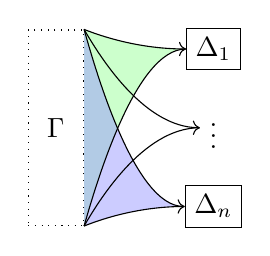
\begin{tikzpicture}[baseline]
    \path
    (-1,1) node (Gtop) {}
    (-1,0) node (G) {$\Gamma$}
    (-1,-1) node (Gbot) {}
    ;
    \node[draw,dotted,fit=(Gtop) (G) (Gbot)] (GG) {};

    \path
    (1,1) node[draw] (Dtop) {$\Delta_1$}
    (1,0) node (D) {$\vdots$}
    (1,-1) node[draw] (Dbot) {$\Delta_n$}
    ;

    \fill[green!20!white,opacity=1] (GG.north east)
    parabola[bend at end] (Dtop.west)
    parabola[bend at start] (GG.south east)
    -- cycle;
    \fill[blue!40!white,opacity=.5] (GG.north east)
    parabola[bend at end] (Dbot.west)
    parabola[bend at start] (GG.south east)
    -- cycle;

    \draw[->] (GG.north east) parabola[bend at end] (Dtop.west);
    \draw (GG.south east) parabola[bend at end] (Dtop.west);
    \draw[->] (GG.north east) parabola[bend at end] (D.west);
    \draw (GG.south east) parabola[bend at end] (D.west);
    \draw[->] (GG.north east) parabola[bend at end] (Dbot.west);
    \draw (GG.south east) parabola[bend at end] (Dbot.west);
  \end{tikzpicture}
\end{displaymath}

To see how this definition works, let us construct an example substitution:
$A, B \to C, B \Longrightarrow B, C$.
Because the codomain is a Cartesian product, it suffices to give two separate
substitutions, $A, B \to C, B \Longrightarrow B$ and
$A, B \to C, B \Longrightarrow C$, with a substitution into a singleton
context being just a term.
We indeed have terms $x : A, y : B \to C, z : B \vdash y : B$ and
$x : A, y : B \to C, z : B \vdash y\,z : C$.
It is also instructive to look at an identity substitution (which is also a
renaming), $A, B \Longrightarrow A, B$, witnessed by terms
$x : A, y : B \vdash x : A$ and $x : A, y : B \vdash y : B$.

When working with our semiring-annotated calculus \name{}, contexts are no
longer understood as Cartesian products.
This means that substitutions of type $\Gamma \Longrightarrow \Delta$ are no
longer equivalent to collections of substitutions
$\Gamma \Longrightarrow \Delta_i$.
Indeed, notice that we should still have an identity substitution of type
$\gr1A, \gr1B \Longrightarrow \gr1A, \gr1B$, but we do not have terms proving
either $\gr1A, \gr1B \vdash A$ or $\gr1A, \gr1B \vdash B$.
What we do have are terms $x : \gr1A, y : \gr0B \vdash x : A$ and
$x : \gr0A, y : \gr1B \vdash y : B$, and if we pointwise add together the
annotations of the two terms, we get back the original context
$x : \gr1A, y : \gr1B$.
Furthermore, adding up the annotations is not just a random operation;
linear contexts are understood to be tensor products of their elements, and
introduction rule for the tensor product involves summing the annotations of
the two sides.

For any annotated context $\Delta$, we have
$\Delta \vdash \bigotimes_{(\gr rx : A) \in \Delta}\oc\gr rA$ by iterated
application of $\otimes$-I with $\oc$-I and Var at the leaves.
Let $\Gamma = \grP\gamma$ and $\Delta = \grQ\delta$.
If we are to produce substitutions from $\Gamma$ to $\Delta$ in this
pattern, we simulate the applications of $\otimes$-I by producing, for each
element in $\Delta$, a usage context for $\gamma$ such that the whole collection
sums to $\grP$, then simulate the applications of $\oc$-I by dividing each of
the new usage contexts by the corresponding annotation in $\Delta$, calling
the divided usage contexts $\gr\Psi_x$, and finally, instead of a variable
from $\delta$, we give a term of type $\gr\Psi_x\gamma \vdash \delta_x$.
In summary, the constraint on the collection of usage contexts $\gr\Psi$ is
that $\grP = \sum_{(\gr rx : A) \in \Delta}\gr r\gr\Psi_x$.
Moreover, if we take $\grP$ and $\grQ$ to be row vectors and $\gr\Psi$ to be a
matrix, the latter expression is equal to the vector-matrix multiplication
$\grQ\gr\Psi$.
The resulting definition of simultaneous substitution is depicted below.

\begin{displaymath}
  \begin{tikzpicture}[baseline]
    \path
    (-1,1) node (Gtop) {}
    (-1,0) node (G) {$\grP\gamma$}
    (-1,-1) node (Gbot) {}
    ;
    \node[draw,dotted,fit=(Gtop) (G) (Gbot)] (GG) {};

    \path
    (1,1) node (Dtop) {}
    (1,0) node (D) {$\grQ\delta$}
    (1,-1) node (Dbot) {}
    ;
    \node[draw,dotted,fit=(Dtop) (D) (Dbot)] (DD) {};

    \draw[->,double] (GG) -- (DD);
  \end{tikzpicture}
  \coloneqq
  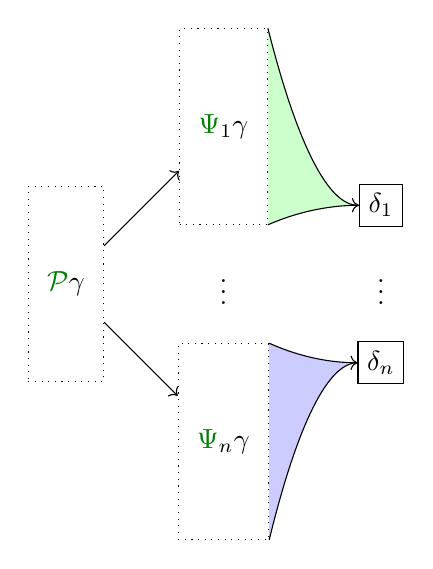
\begin{tikzpicture}[baseline]
    \path
    (-1,1) node (Gtop) {}
    (-1,0) node (G) {$\grP\gamma$}
    (-1,-1) node (Gbot) {}
    ;
    \node[draw,dotted,fit=(Gtop) (G) (Gbot)] (GG) {};

    \path
    (1,3) node (G1top) {}
    (1,2) node (G1) {$\gr\Psi_1\gamma$}
    (1,1) node (G1bot) {}
    ;
    \node[draw,dotted,fit=(G1top) (G1) (G1bot)] (GG1) {};
    \draw[->] (GG) -- (GG1);

    \path (1,0) node {$\vdots$};

    \path
    (1,-1) node (Gntop) {}
    (1,-2) node (Gn) {$\gr\Psi_n\gamma$}
    (1,-3) node (Gnbot) {}
    ;
    \node[draw,dotted,fit=(Gntop) (Gn) (Gnbot)] (GGn) {};
    \draw[->] (GG) -- (GGn);

    \path
    (3,1) node[draw] (Dtop) {$\delta_1$}
    (3,0) node (D) {$\vdots$}
    (3,-1) node[draw] (Dbot) {$\delta_n$}
    ;

    \fill[green!20!white] (GG1.north east)
    parabola[bend at end] (Dtop.west)
    parabola[bend at start] (GG1.south east)
    -- cycle;
    \draw[->] (GG1.north east) parabola[bend at end] (Dtop.west);
    \draw (GG1.south east) parabola[bend at end] (Dtop.west);

    \fill[blue!20!white] (GGn.north east)
    parabola[bend at end] (Dbot.west)
    parabola[bend at start] (GGn.south east)
    -- cycle;
    \draw[->] (GGn.north east) parabola[bend at end] (Dbot.west);
    \draw (GGn.south east) parabola[bend at end] (Dbot.west);
  \end{tikzpicture}
  \quad\textrm{where }\grP = \grQ\gr\Psi
\end{displaymath}

In type theory, we write out the definition as follows.

\begin{displaymath}
  \sum_{\gr\Psi : \size\Delta \to \size\Gamma \to \Ann}
    \left(\grP = \grQ\gr\Psi\right) \times
    \prod_{(x : A) \in \delta}\gr\Psi_x\gamma \vdash A
\end{displaymath}

We can see the step-by-step construction of a substitution play out by adapting
the previous example to have type
$\gr0A, \gr2(B \multimap C), \gr3B \Longrightarrow \gr1B, \gr2C$.
To split the goal up, we note that $
\begin{pmatrix} \gr0 & \gr2 & \gr3 \end{pmatrix} =
\begin{pmatrix} \gr0 & \gr0 & \gr1 \end{pmatrix} +
\begin{pmatrix} \gr0 & \gr2 & \gr2 \end{pmatrix}
$, so it suffices to give substitutions of types
$\gr0A, \gr0(B \multimap C), \gr1B \Longrightarrow \gr1B$ and
$\gr0A, \gr2(B \multimap C), \gr2B \Longrightarrow \gr2C$.
Furthermore, our term calculus only supports $\gr1$-annotated conclusions,
so we divide the second substitution type through by $\gr2$.
Finally, we give the terms largely as before:
$\gr0x : A, \gr0y : B \to C, \gr1z : B \vdash y : B$ and
$\gr0x : A, \gr1y : B \to C, \gr1z : B \vdash z\,y : C$.

While we naturally derive a matrix as a fragmentation of a usage vector, we can
get a slightly cleaner presentation by instead using an abstract linear map.
Let $\gr\Psi$ now be a linear map of type
$\Ann^{\size\Delta} \to \Ann^{\size\Gamma}$, with application written postfix.
The equation $\grP = \grQ\gr\Psi$ remains unchanged.
Where we previously wrote $\gr\Psi_x$, the most direct replacement would be
$\langle x \rvert\gr\Psi$, with $\langle x \rvert$ being the $x$th basis row
vector.
But then we notice that $\langle x \rvert$ is exactly the $\grQprime$ satisfying
$\grQprime\delta \sqni x : B$.
This gives us the following definition, which can be verified by equationally
substituting $\grPprime$ and expanding the definition of $\sqni$.

\begin{displaymath}
  \sum_{\gr\Psi : \Ann^{\size\Delta} \to \Ann^{\size\Gamma}}
    \left(\grP = \grQ\gr\Psi\right) \times
    \prod_{A,\grQprime,\grPprime} \left(
    \grPprime = \grQprime\gr\Psi \to \grQprime\delta \sqni A \to
    \grPprime\gamma \vdash A\right)
\end{displaymath}

We now have a new reading for the interpretation of a linear substitution:
a linear map $\gr\Psi$ relating the two usage vectors $\grP$ and $\grQ$, and
for any two similarly related usage vectors $\grPprime$ and $\grQprime$, we
have a type-preserving function from variables in $\grQprime\delta$ to terms in
$\grPprime\gamma$.
Even though we don't use $\gr\Psi$ as a matrix containing fragmented usage
vectors, we can still justify why it should be a \emph{linear} map.
We need $\gr\Phi$ to respect all fragmentation of the usage context in a typing
rule, and we know that all such fragmentation is done by linear operations
zero, addition, and scaling by a constant.
\todo{Expand. Substitutions need to preserve everything done to the context,
and linear things are all we do to the context.}

Taking a lead from \cref{sec:kits}, we deduce a definition of
\emph{environment} by replacing the $\vdash$ in the definition of simultaneous
substitution by an arbitrary type family $\mathcal V$.
Letting $\mathcal V$ be $\sqni$ gives us a notion of simultaneous renaming,
allowing for renamings with types such as
$\gr6A, \gr0B, \gr1C \stackrel\sqni\Longrightarrow \gr1C, \gr2A, \gr4A$.

It is worth noting that, when contexts are Cartesian products, passing from
``a map into $\Delta$'' to ``for each $A \in \Delta$, a map into $A$'' does not
lose any generality because the universal property of Cartesian products
states that every map into a Cartesian product can be given factor-wise.
Hence, $\Delta$ and the one-element context $\prod_{A \in \Delta}A$ are
isomorphic in the category of contexts and simultaneous substitution.
However, tensor products are not limits, so don't have the same universal
property.
Indeed, many annotated contexts are not isomorphic to the weighted product of
their elements.
For example, we do not have a substitution of type
$\gr1(A \otimes B) \Longrightarrow \gr1A, \gr1B$ because we would first need
to pattern-match on the tensor product \emph{before} trying to derive the
target context.
This loss of generality is however justified when we consider the action of a
substitution.
Substitutions should only be replacing variables by terms, whereas if
substitutions were allowed to pattern-match before introducing the target, then
the substitution would have to replace the original term by a term that first
pattern-matches and then continues like the original term.
\label{sec:lrkits}
  \section{Properties of linear environments}
  \begin{remark}
  Given an environment $\rho : \grP\gamma \env\V \grQ\delta$ and a $\grPprime$
  and a $\grQprime$ such that $\grPprime = \grQprime\plr{\rho.\gr\Psi}$,
  there is also an environment of type $\grPprime\gamma \env\V \grQprime\delta$
  with the same linear map and action on variables.
\end{remark}
\begin{proof}
  The only part of the definition of an environment dependent on $\grP$ or
  $\grQ$ is the constraint $\grP = \grQ\gr\Psi$, which we are able to replace
  for $\grPprime$ and $\grQprime$.
\end{proof}

When constructing an environment, we can do so by cases on the shape of the
target context.
We can create an environment into the empty context when all usage annotations
on the source context are $\gr0$.
We can create an environment into a concatenated context when we can additively
split up the annotations of the source context and produce environments into
both halves from the split sources.
We can create an environment into a singleton context when there is a context
$\gr r$ times smaller than the source context in which we can produce a value
of the appropriate type.

\begin{lemma}\label{thm:construct-env}
  We can define all of the following equivalences for any values of the free
  variables.
  \begin{itemize}
    \item $\forallb{I \dotlr \plr{{-} \env\V {\cdot}}}$
    \item $\forallb{\plr{{-} \env\V \Gamma} \sep \plr{{-} \env\V \Delta}
      \dotlr \plr{{-} \env\V \Gamma, \Delta}}$
    \item
      $\forallb{\gr r \cdot \plr{\V\,(-)\,A} \dotlr \plr{{-} \env\V \gr rA}}$
  \end{itemize}
\end{lemma}
\begin{proof}
  There are 6 cases to check.
  Throughout, we write $\Gamma$ as $\grP\gamma$ and $\Delta$ as $\grQ\delta$
  when convenient.
  \begin{description}
    \item[$I(\to)$]
      Let $\gr\Psi$ be the unique linear map out of the zero space.
      By definition, $\gr0 = \grQ\gr\Psi$.
      There are no variables to act upon.
    \item[$I(\gets)$]
      $\grQ\gr\Psi$ is an empty sum, so if $\grP = \grQ\gr\Psi$ then
      $\grP = \gr0$.
    \item[$\sep(\to)$]
      Let the given environments be $\rho : \grRl\theta \env\V \Gamma$ and
      $\sigma : \grRr\theta \env\V \Delta$, with $\grR = \grRl + \grRr$.
      Define $\gr\Psi \coloneqq [\rho.\gr\Psi, \sigma.\gr\Psi]$, using the
      coproduct structure of the concatenated vector space.
      We have $\grR = \grRl + \grRr =
      \grP\plr{\rho.\gr\Psi} + \grQ\plr{\sigma.\gr\Psi} =
      \plr{\grP, \grQ}\gr\Psi$.
      To act on variables, we are given
      $\grRprime = \plr{\grPprime, \grQprime}\gr\Psi$ and
      $\grPprime\gamma, \grQprime\delta \sqni A$.
      Without loss of generality, let us have $\grPprime\gamma \sqni A$ and
      $\grQprime = \gr0$.
      Thus, $\grRprime = \grPprime\plr{\rho.\gr\Psi}$, and we can act on the
      variable using $\rho$.
    \item[$\sep(\gets)$]
      Let the unnamed context be $\Theta$, also written $\grR\theta$.
      The linear map
      $\gr\Psi : \Ann^{\size\Gamma + \size\Delta} \to \Ann^{\size\Theta}$ splits
      into
      $\gr\Psi_{\gr l} : \Ann^{\size\Gamma} \to \Ann^{\size\Theta}
      \coloneqq \langle \id, 0 \rangle; \gr\Psi$ and
      $\gr\Psi_{\gr r} : \Ann^{\size\Delta} \to \Ann^{\size\Theta}
      \coloneqq \langle 0, \id \rangle; \gr\Psi$, using the product structure of
      the concatenated vector space.
      Let $\grRl \coloneqq \grP\gr\Psi_{\gr l}$ and
      $\grRr \coloneqq \grQ\gr\Psi_{\gr r}$, by definition satisfying the
      required equations.
      For the action on variables, let us consider the left environment.
      We are given $\grRprime = \grPprime\gr\Psi_{\gr l}$ and
      $\grPprime\gamma \sqni A$.
      From these, we get
      $\grRprime = \grPprime\gr\Psi_{\gr l} = \plr{\grPprime, \gr0}\gr\Psi$ and
      $\grPprime\gamma, \gr0\delta \sqni A$.
      We can therefore act using the original environment.
    \item[$\cdot(\to)$]
      Let $\grP$ and $\grPprime$ be such that $\grP = \gr r\grPprime$ and let
      $v : \V\,\grPprime\gamma\,A$.
      Let $\gr\Psi : \Ann \to \Ann^{\size\gamma}
      \coloneqq \gr r\gr' \mapsto \gr r\gr'\grPprime$.
      By definition and the previous assumption, we have $\grP = \gr r\gr\Psi$.
      When acting on a variable, we have $\grP\gr{''} = \gr r\gr'\gr\Psi$
      and $\gr r\gr'A \sqni A'$.
      The latter tells us that $A = A'$ and $\gr r\gr' = \gr1$.
      Thus, $\grP\gr{''} = \grPprime$.
      We therefore need a value of type $\V\,\grPprime\gamma\,A$, which we can
      take to be $v$.
    \item[$\cdot(\gets)$]
      Let us have an environment of type $\grP\gamma \env\V \gr rA$.
      We want to use its action on variables to yield a value.
      To do this, we let $\grPprime \coloneqq \gr1\gr\Psi$, and use this
      equation, together with the fact that we have a variable of type
      $\gr1A \sqni A$, to get a value of type $\V\,\grPprime\gamma\,A$.
      Furthermore, we derive $\grP = \gr r\gr\Psi = \gr r\grPprime$, as
      required.
  \end{description}
\end{proof}

We could, indeed, use these three clauses to define what an environment is.
However, I find them difficult to work with, as it is often easier to do
linear algebraic proofs separately from the rest of an environment.
For identity and composition, as we are about to see, the original definition
is easier to use because we can rely on the identity and composition of linear
maps.
Concretely, an inductive proof of identity would, for example, involve
constructing an environment of type
$\grP\gamma, \grQ\delta \env\V \grP\gamma, \grQ\delta$ by constructing
environments of types $\grP\gamma, \gr0\delta \env\V \grP\gamma$ and
$\gr0\gamma, \grQ\delta \env\V \grQ\delta$.
These are not identity environments, so we would have to strengthen the
induction hypothesis.

One of the primary test cases for environments is simultaneous substitution,
which will look like the following rule.
The admissibility of substitution will be by induction on the derivation of
$\Delta \vdash A$, so we will need to be able to adapt any environment we are
given to work with any possible context of new premises.
In the simply typed case, the only change to the context we encountered was the
binding of new variables.
Now, with usage annotations, we furthermore have linear decompositions of the
context, necessitating changes to the environment whenever usage annotations
change.
I will deal first with linear decompositions.

\begin{displaymath}
  \begin{prooftree}
    \hypo{\Gamma \env{\vdash} \Delta}
    \hypo{\Delta \vdash A}
    \infer2[sub]{\Gamma \vdash A}
  \end{prooftree}
\end{displaymath}

There are three kinds of linear decompositions we have to deal with: zero,
addition, and scaling; corresponding to bunched connectives $I^*$, $\sep$, and
$\gr r \cdot {}$, respectively.
In each case, we have a simple preservation lemma, transforming an environment
of type $\Gamma \env\V \Delta$ and a decomposition of $\Delta$ into a
decomposition of $\Gamma$ and environments for all of the decomposed fragments
of $\Gamma$ and $\Delta$.

\begin{lemma}[environments preserve zero]\label{thm:lr-env-zero}
  Given an environment of type $\grP\gamma \env\V \grQ\delta$ such that
  $\grQ \leq \gr 0$, we also have that $\grP \leq \gr 0$.
\end{lemma}
\begin{proof}
  $\grP \leq \grQ\gr\Psi \leq \gr0\gr\Psi = \gr0$, by environment
  compatibility and monotonicity and linearity of $\gr\Psi$.
\end{proof}

\begin{lemma}[environments preserve addition]\label{thm:lr-env-add}
  Given an environment of type $\grP\gamma \env\V \grQ\delta$ such that
  $\grQ \leq \grQl + \grQr$ for some $\grQl$ and $\grQr$, we also have $\grPl$
  and $\grPr$ such that $\grP \leq \grPl + \grPr$ and there are environments
  of types $\grPl\gamma \env\V \grQl\delta$ and
  $\grPr\gamma \env\V \grQr\delta$.
\end{lemma}
\begin{proof}
  Let $\grPl \coloneqq \grQl\gr\Psi$ and $\grPr \coloneqq \grQr\gr\Psi$.
  Then, $\grP \leq \grQ\gr\Psi \leq \plr{\grQl + \grQr}\gr\Psi =
  \grQl\gr\Psi + \grQr\gr\Psi = \grPl + \grPr$, satisfying the first condition.
  Because clearly $\grPl \leq \grQl\gr\Psi$ and $\grPr \leq \grQr\gr\Psi$,
  \cref{thm:env-resize} on the original environment gives us the required
  pair of new environments.
\end{proof}

\begin{lemma}[environments preserve scaling]\label{thm:lr-env-scale}
  Given an environment of type $\grP\gamma \env\V \grQ\delta$ such that
  $\grQ \leq \gr r\grQprime$ for some $\grQprime$, we also have a $\grPprime$
  such that $\grP \leq \gr r\grPprime$ and there is an environment of type
  $\grPprime\gamma \env\V \grQprime\delta$.
\end{lemma}
\begin{proof}
  Let $\grPprime \coloneqq \grQprime\gr\Psi$.
  Then, $\grP \leq \grQ\gr\Psi \leq \plr{\gr r\grQprime}\gr\Psi =
  \gr r\plr{\grQprime\gr\Psi} = \gr r\grPprime$, satisfying the first condition.
  Because clearly $\grPprime \leq \grQprime\gr\Psi$,
  \cref{thm:env-resize} on the original environment gives us the required
  new environment.
\end{proof}

Finally, I will also take the opportunity to give the bind lemma, allowing
environments to incorporate newly bound variables.
In the intuitionistic case, the bind lemma had two requirements on $\V$: $\V$
admits weakening and we can map variables into $\V$-values.
With usage annotations, the former is unreasonable, but it turns out that we
only need weakening by variables whose usage annotation is less than or equal
to $\gr0$.
The latter stays as-is, with the note that ``variable'' now means a
usage-checked variable.

\begin{lemma}[bind]\label{thm:lr-bind}
  Given functions
  ${\swarrow^k} : \forall \Gamma, \grR, \theta.~\grR \leq \gr0 \to
  \forallb{\V\,\Gamma \dotto \V\,\plr{\Gamma, \grR\theta}}$ and
  $\mathrm{vr} : \forallb{{\sqni} \dotto \V}$, we can turn an environment of
  type $\Gamma \env\V \Delta$ into an environment of type
  $\Gamma, \Theta \env\V \Delta, \Theta$ for any context $\Theta$.
\end{lemma}
\begin{proof}
  Let $\grP\gamma \coloneqq \Gamma$, $\grQ\delta \coloneqq \Delta$, and
  $\grR\theta \coloneqq \Theta$.
  Let the new linear map $\gr\Psi\gr' : \Ann^{\size\Delta + \size\Theta} \to
  \Ann^{\size\Gamma + \size\Theta}$ be $\gr\Psi \oplus \gr I$.
  That is, in block matrix notation,
  $\begin{pmatrix} \gr\Psi & \gr0 \\ \gr0 & \gr I \end{pmatrix}$.
  Checking that this linear map fits, we have
  $\begin{pmatrix}\grP & \grR\end{pmatrix}
  \leq \begin{pmatrix}\grQ\gr\Psi & \grR\gr I\end{pmatrix}
  = \begin{pmatrix}\grQ & \grR\end{pmatrix}\plr{\gr\Psi \oplus \gr I}$.
  For the action on variables, we are given vectors $\grPprime$,
  $\grR\gr'_\grP$, $\grQprime$, and $\grR\gr'_\grQ$ such that
  $\begin{pmatrix} \grPprime & \grR\gr'_\grP \end{pmatrix} \leq
  \begin{pmatrix} \grQprime & \grR\gr'_\grQ \end{pmatrix}
  \plr{\gr\Psi \oplus \gr I}$ and we have a variable of type
  $\grQprime\delta, \grR\gr'_\grQ\theta \sqni A$ for some type $A$.
  The constraint on the new vectors reduces to $\grPprime \leq \grQprime\gr\Psi$
  and $\grR\gr'_\grP \leq \grR\gr'_\grQ$.
  From the variable we either have a variable $x$ in $\delta$ with
  $\grQprime \leq \langle x \rvert$ and $\grR\gr'_\grQ \leq \gr0$, or a
  variable $y$ in $\theta$ with $\grQprime \leq \gr0$ and
  $\grR\gr'_\grQ \leq \langle y \rvert$.
  In the former case, the action of the original environment on $x$ gives us a
  $\V$-value in $\grPprime\gamma$, and the $\gr0$-weakening principle
  $\swarrow^k$, noting that $\grR\gr'_\grP \leq \grR\gr'_\grQ \leq \gr0$, gives
  us a $\V$-value in $\grPprime\gamma, \grR\gr'_\grP\theta$.
  In the latter case, we have that
  $\begin{pmatrix} \grPprime & \grR\gr'_\grP \end{pmatrix}
  \leq \begin{pmatrix} \grQprime\gr\Psi & \grR\gr'_\grQ \end{pmatrix}
  \leq \begin{pmatrix} \gr0\gr\Psi & \langle y \rvert \end{pmatrix}
  = \begin{pmatrix} \gr0 & \langle y \rvert \end{pmatrix}
  = \left\langle {\searrow}y \right\rvert$, so $y$ also serves as a
  usage-checked variable in $\grPprime\gamma, \grR\gr'_\grP\theta$.
  From this usage-checked variable, we get a $\V$-value in the same context
  using $\mathrm{vr}$.
\end{proof}

The requirements for identity and composition of environments look a bit like
the unit and lift of a Kleisli triple.

\begin{lemma}[Identity environment]
  Given a function $\mathrm{vr} : \forallb{{\sqni} \dotto \V}$, for any
  $\Gamma$ we have an environment of type $\Gamma \env\V \Gamma$.
\end{lemma}
\begin{proof}
  Let $\gr\Psi$ be the identity map, which clearly satisfies
  $\grP = \grP\gr\Psi$.
  When acting on a variable, the equation $\grPprime = \grQprime\gr\Psi$ means
  that $\grPprime = \grQprime$, so we want, from a variable of type
  $\grPprime\gamma \sqni A$, a value of type $\V\,\grPprime\gamma\,A$, which
  we can get from $\mathrm{vr}$.
\end{proof}

\begin{lemma}\label{thm:env-comp-lemma}
  Given an environment $\rho : \Gamma \env\U \Delta$ for which we have, for any
  $\grPprime$ and $\grQprime$ such that
  $\grPprime = \grQprime\plr{\rho.\gr\Psi}$, we have a function
  $\mathrm{lift}_\rho :
  \forallb{\V\,\grQprime\delta \dotto \W\,\grPprime\gamma}$,
  we can map environments of type $\Delta \env\V \Theta$ into environments of
  type $\Gamma \env\W \Theta$.
\end{lemma}
\begin{proof}
  Let $\rho$ be as in the statement, and let $\sigma : \Delta \env\V \Theta$.
  For the environment we are constructing, let
  $\gr\Psi \coloneqq \sigma.\gr\Psi; \rho.\gr\Psi$, noting that
  $\grP = \grQ\plr{\rho.\gr\Psi} =
  \plr{\grR\plr{\sigma.\gr\Psi}}\plr{\rho.\gr\Psi}$.
  For the action on variables, we are given $\grPprime = \grRprime\gr\Psi$ with
  $\grRprime\theta \sqni A$.
  We can immediately apply the action of $\sigma$, giving us a value of type
  $\V\,\plr{\grRprime\plr{\sigma.\gr\Psi}}\,A$.
  We note that
  $\grPprime = \plr{\grRprime\plr{\sigma.\gr\Psi}}\plr{\rho.\gr\Psi}$, and
  apply $\mathrm{lift}_\rho$ to get the desired value.
\end{proof}

\begin{corollary}[Composition of environments]
  Given a function
  $\mathrm{lift} : \plr{\rho : \grP\gamma \env\U \grQ\delta} \to
  \forall \grPprime, \grQprime.~\grPprime = \grQprime\plr{\rho.\gr\Psi} \to
  \forallb{\V\,\grQprime\delta \dotto \W\,\grPprime\gamma}$, then we can
  compose environments of types $\Gamma \env\U \Delta$ and
  $\Delta \env\V \Theta$ into an environment of type $\Gamma \env\W \Theta$.
\end{corollary}

\begin{example}
  We can derive the following instances of environment composition.
  \begin{itemize}
    \item If $\U = \V = \W = {\sqni}$, then $\mathrm{lift}$ is given by the
      action of the renaming $\rho$ on variables.
      This allows us to derive composition of renamings.
    \item More generally, if $\V = {\sqni}$ and $\U = \W$, we can still use
      the action of the environment $\rho$.
      This means that renamings post-compose with any other sort of environment.
    \item If $\V = \W = {\vdash}$, then $\mathrm{lift}$ is given by a
      syntactic traversal.
      For example, if $\U = {\sqni}$, we need the action of renaming on terms
      to show that a renaming followed by a substitution composes to a
      substitution.
      If $\U = {\vdash}$, then the action of substitution on terms gives us that
      substitutions compose.
    \item More generally, if $\V = {\vdash}$ and we have a semantics from
      $\U$ to $\W$, then $\mathrm{lift}$ can be given by the semantic traversal
      of terms.
  \end{itemize}
\end{example}

% Concatenation is difficult; save to after I've talked about renamings.

% Finally for this section, we give the conditions under which the
% context-forming operations (empty, concatenation, and singleton) have a
% functorial action with respect to $\V$-environments.
%
% \begin{lemma}
%   For any $\V$, there is an environment ${\cdot} \env\V {\cdot}$.
% \end{lemma}
% \begin{proof}
%   By \autoref{thm:construct-env}, it suffices to show $I\,{\cdot}$, which is
%   trivially true.
% \end{proof}
\label{sec:lenv}
  \section{Substitution is admissible in \name{}}
  \def\LRKits{../agda/processed-latex/LRKits.tex}

I can now show that, using the notion of \emph{environment} derived in
\cref{sec:lrkits}, we can replicate the Agda proofs from
\cref{sec:syntactic-kits} in the usage-aware setting of $\name$.
From \cref{sec:lenv}, we know that environments are preserved under all
syntax-forming operations: zero, addition, scaling, and binding.
What is left is to show how these properties are deployed, and also how to
go on and prove the admissibility of simultaneous renaming, simultaneous
substitution, and then single substitution.

There are a few notational changes necessary in the Agda code, compared to the
typeset mathematics above.
Usage vectors, elsewhere called $\grP$, $\grQ$, and $\grR$ are rendered as
\AgdaBound{P}, \AgdaBound{Q}, and \AgdaBound{R}, respectively.
Usage contexts and typing contexts are tied together with the
\AgdaInductiveConstructor{ctx} constructor, rather than simple juxtaposition.
Environments, elsewhere notated $\Gamma \env\V \Delta$, are rendered as
\AgdaRecord{[}\AgdaSpace{}\AgdaBound{$\V$}\AgdaSpace{}\AgdaRecord{]}%
\AgdaSpace{}\AgdaBound{$\Gamma$}\AgdaSpace{}\AgdaRecord{$\Rightarrow^e$}%
\AgdaSpace{}\AgdaBound{$\Delta$}.

We start with a slightly modified definition of \AgdaRecord{Kit}.
We saw in \cref{thm:lr-bind} that in the usage-annotated context, we restrict
weakening of $\V$-values to just $\gr0$-use variables.
Meanwhile, the function $\mathrm{vr}$, also seen in \cref{thm:lr-bind}, maps
usage-checked variables to $\V$-values, and the function $\mathrm{tm}$, used
to coerce $V$-values yielded by the environment into terms, stays the same.
I state weakening in a slightly different way than previously, so as to help
unification against a known result type (avoiding the problem described by
\citet{McBride12} as \emph{green slime}).
The type \AgdaFunction{Weakening}\AgdaSpace{}\AgdaBound{$\V$} can be read as
saying that, for any context $\grP\gamma$ of shape $s + t$, if the right of
$\grP$ is below $\gr0$, then a value in the left part of $\grP\gamma$ weakens
to a value in the whole of $\grP\gamma$.

\ExecuteMetaData[\LRKits]{Kit}

To demonstrate the important points succinctly, I cut \name{} down to just the
$\oc\gr r$-fragment.
The introduction rule and pattern-matching eliminator feature scaling, addition,
and variable binding, missing out only on sharing (which is trivial) and zero
(which is simpler than, and analogous to, addition).
The resulting type of well typed terms is below.

\ExecuteMetaData[\LRKits]{Tm}

Given a \AgdaRecord{Kit}, \cref{thm:lr-bind} looks like the following.
The \AgdaField{lookup} clauses still contain essentially the same structure as
in the intuitionistic case: discriminating on whether the variable is old or
new, using the given environment \AgdaBound{$\rho$} and weakening on the old
variables, and using \AgdaField{vr} to repackage new variables.
I will not explain any of the algebraic manipulations here; see
\cref{thm:lr-bind}.

\ExecuteMetaData[\LRKits]{bindEnv}

Given \AgdaFunction{bindEnv} (\cref{thm:lr-bind}), \AgdaFunction{env-+}
(\cref{thm:lr-env-add}), and \AgdaFunction{env-*} (\cref{thm:lr-env-scale}),
we can reproduce the syntactic traversal \AgdaFunction{trav}.
With all these lemmas in place, writing \AgdaFunction{trav}
becomes routine.
When processing a rule, we work our way up through the
premise connectives, applying \AgdaFunction{env-*} wherever we see a
\AgdaFunction{$\cdot^c$}, \AgdaFunction{env-+} wherever we see a
\AgdaFunction{$*^c$}, and \AgdaFunction{bindEnv} wherever we see a
\AgdaFunction{Bind}.
We then use whatever environments (with names beginning with
\AgdaBound{$\rho$}) and whatever usage vector splitting facts (with names
beginning with \AgdaBound{sp}) come out of this process to recursively
traverse the subterms and recombine the results.

\ExecuteMetaData[\LRKits]{trav}

Instantiating the generic syntactic traversal \AgdaFunction{trav} to renaming
looks just like it did in the intuitionistic case.
I have consistently replaced intuitionistic variables by linear variables, so
\AgdaFunction{id} and \AgdaInductiveConstructor{var} still work to embed
variables into variables and terms, respectively.
Weakening for variables \AgdaFunction{$\swarrow^v$} (not pictured) has been
updated to note that, for $\grP \leq \bra x$ and $\grR \leq \gr0$, we also have
$\begin{pmatrix} \grP & \grR \end{pmatrix} \leq \bra{{\swarrow}x}$.

\ExecuteMetaData[\LRKits]{var-kit}

In the intuitionistic case, environments were just functions, so we passed the
variable weakening function \AgdaFunction{$\swarrow^v$} to the function
\AgdaFunction{ren} to yield a term weakening function.
However, a usage-aware environment is a function packed together with usage
distribution data.
As such, we must make an environment version of \AgdaFunction{$\swarrow^v$}.
I start with a general lemma \AgdaFunction{$\swarrow$\^{}Env}, stating that if
$\V$ supports weakening, then so do $\V$-environments (in their domain
context).
This lemma then specialises to variables, with the identity renaming
\AgdaFunction{id\^{}Env} on the left part of the context and the proof
\AgdaBound{R0} that the right part of the context is below $\gr0$ combining
to give the desired weakening environment.

\ExecuteMetaData[\LRKits]{dlv-env}

This is what we need to instantiate \AgdaFunction{trav} for substitution.
As a reminder, I also give the type of \AgdaFunction{sub} in rule form.

\ExecuteMetaData[\LRKits]{sub}
\[
  \ebrule{%
    \hypo{\Gamma \env\vdash \Delta}
    \hypo{\Delta \vdash B}
    \infer2[sub]{\Gamma \vdash B}
  }
\]

Finally, the simultaneous substitution \AgdaFunction{sub} specialises to
single substitution \AgdaFunction{sub[-]}.
Single substitution is stated as an admissible rule below.
To substitute in for $\gr r$-many $A$ in the second term, we need to derive
one $A$ with usages $\grP$, and then assert that the result can handle the
usages of the original term $\grQ$, plus $\gr r$-many copies of $\grP$.

\[
  \ebrule{%
    \hypo{\grR \leq \grQ + \gr r\grP}
    \hypo{\grP\gamma \vdash A}
    \hypo{\grQ\gamma, \gr rA \vdash B}
    \infer3[singleSub]{\grR\gamma \vdash B}
  }
\]

The proof strategy for producing the substitution \AgdaFunction{$\sigma$} is
to proceed structurally on the codomain context $\grQ\gamma, \gr rA$ using
\cref{thm:construct-env}, applying the identity substitution
\AgdaFunction{id\^{}Env} on the $\gamma$ half, and dropping the term
\AgdaBound{t} in place of the variable we are substituting for.

\ExecuteMetaData[\LRKits]{subSingle}


\chapter{Weighted multicategories}
  \section{Ordinary and Cartesian multicategories}
  In type theory and categorical logic, the idea of multicategories is to give
an algebraic structure that is close to the syntax of type theory.
In simple type theory, sequents take the form $\Gamma \vdash A$, where $A$ is
the type of the conclusion and $\Gamma$ is a list of types, one type for each
assumption.
Intuitively, a term with assumptions $\Gamma$ and type $A$ constitutes a
morphism from $\Gamma$ to $A$.
Multicategories make this structure --- domains being lists of objects and
codomains being a single object --- part of the definition of morphisms.

\begin{definition}[multicategory]
  A \emph{multicategory} comprises a collection of objects $\obj$, for each
  list of objects $\Gamma$ and object $A$ a set of (multi)morphisms
  $\hom(\Gamma, A)$, and the following morphisms, satisfying the following
  axioms.

  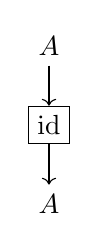
\begin{tikzpicture}
    \path
    (0,1) node(s) {$A$}
    (0,0) node[draw](id) {$\id$}
    (0,-1) node(t) {$A$}
    ;

    \draw[->] (s) -- (id);
    \draw[->] (id) -- (t);
  \end{tikzpicture}
  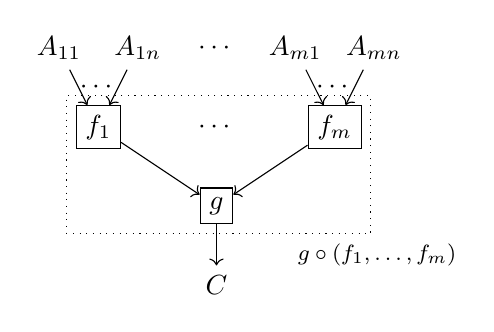
\begin{tikzpicture}
    \path
    (-2,2) node(A11) {$A_{11}$}
    (-1.5,1.5) node(A1dots) {$\cdots$}
    (-1,2) node(A1n) {$A_{1n}$}
    (0,2) node(Adots) {$\cdots$}
    (1,2) node(Am1) {$A_{m1}$}
    (1.5,1.5) node(Amdots) {$\cdots$}
    (2,2) node(Amn) {$A_{mn}$}

    (-1.5,1) node[draw](f1) {$f_1$}
    (0,1) node(fdots) {$\cdots$}
    (1.5,1) node[draw](fm) {$f_m$}

    (0,0) node[draw](g) {$g$}

    (0,-1) node(C) {$C$}
    ;

    \node[draw,dotted,fit=(f1) (fm) (g),
    label=below right:{\footnotesize$g \circ (f_1, \ldots, f_m)$}] (box) {};

    \draw[->] (A11) -- (f1);
    \draw[->] (A1n) -- (f1);
    \draw[->] (Am1) -- (fm);
    \draw[->] (Amn) -- (fm);
    \draw[->] (f1) -- (g);
    \draw[->] (fm) -- (g);
    \draw[->] (g) -- (C);
  \end{tikzpicture}

  \begin{displaymath}
    \begin{matrix}
      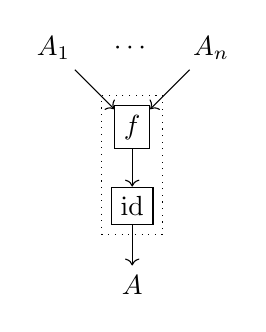
\begin{tikzpicture}[baseline]
        \path
        (-1,2) node(A1) {$A_1$}
        (0,2) node(Adots) {$\cdots$}
        (1,2) node(An) {$A_n$}
        (0,1) node[draw](f) {$f$}
        (0,0) node[draw](id) {$\id$}
        (0,-1) node(t) {$A$}
        ;

        \node[draw,dotted,fit=(f) (id)] {};

        \draw[->] (A1) -- (f);
        \draw[->] (An) -- (f);
        \draw[->] (f) -- (id);
        \draw[->] (id) -- (t);
      \end{tikzpicture}
      =
      \begin{tikzpicture}[baseline]
        \path
        (-1,1) node(A1) {$A_1$}
        (0,1) node(Adots) {$\cdots$}
        (1,1) node(An) {$A_n$}
        (0,0) node[draw](f) {$f$}
        (0,-1) node(t) {$A$}
        ;

        \draw[->] (A1) -- (f);
        \draw[->] (An) -- (f);
        \draw[->] (f) -- (t);
      \end{tikzpicture}
      &\phantom{mmmm}&
      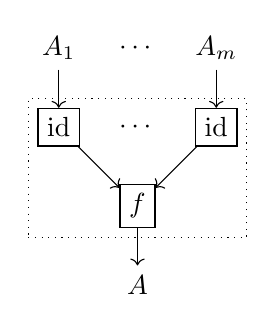
\begin{tikzpicture}[baseline]
        \path
        (-1,2) node(A1) {$A_1$}
        (0,2) node(Adots) {$\cdots$}
        (1,2) node(Am) {$A_m$}
        (-1,1) node[draw](id1) {$\id$}
        (0,1) node(iddots) {$\cdots$}
        (1,1) node[draw](idm) {$\id$}
        (0,0) node[draw](f) {$f$}
        (0,-1) node(t) {$A$}
        ;

        \node[draw,dotted,fit=(id1) (idm) (f)] {};

        \draw[->] (A1) -- (id1);
        \draw[->] (Am) -- (idm);
        \draw[->] (id1) -- (f);
        \draw[->] (idm) -- (f);
        \draw[->] (f) -- (t);
      \end{tikzpicture}
      =
      \begin{tikzpicture}[baseline]
        \path
        (-1,1) node(A1) {$A_1$}
        (0,1) node(Adots) {$\cdots$}
        (1,1) node(An) {$A_n$}
        (0,0) node[draw](f) {$f$}
        (0,-1) node(t) {$A$}
        ;

        \draw[->] (A1) -- (f);
        \draw[->] (An) -- (f);
        \draw[->] (f) -- (t);
      \end{tikzpicture}
    \end{matrix}
  \end{displaymath}

  \begin{displaymath}
    \begin{matrix}
      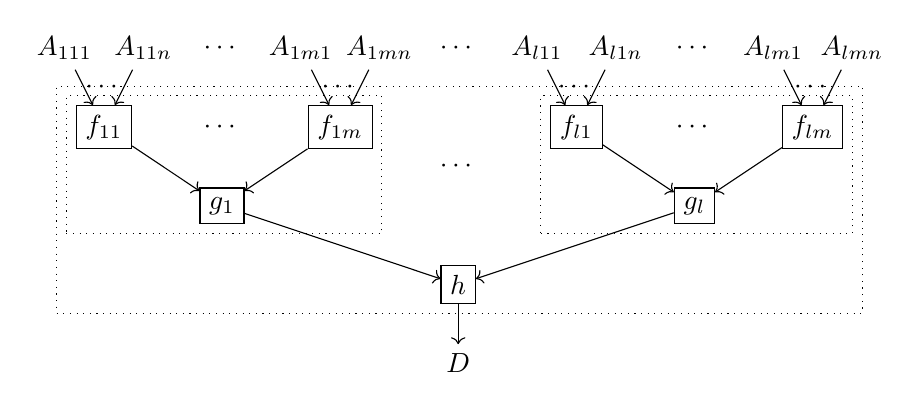
\begin{tikzpicture}
        \path
        % left
        (-5,2) node(A111) {$A_{111}$}
        (-4.5,1.5) node(A1dots) {$\cdots$}
        (-4,2) node(A11n) {$A_{11n}$}
        (-3,2) node(Adots) {$\cdots$}
        (-2,2) node(A1m1) {$A_{1m1}$}
        (-1.5,1.5) node(Amdots) {$\cdots$}
        (-1,2) node(A1mn) {$A_{1mn}$}

        (-4.5,1) node[draw](f11) {$f_{11}$}
        (-3,1) node(fdots) {$\cdots$}
        (-1.5,1) node[draw](f1m) {$f_{1m}$}

        (-3,0) node[draw](g1) {$g_1$}

        % right
        (1,2) node(Al11) {$A_{l11}$}
        (1.5,1.5) node(A1dots) {$\cdots$}
        (2,2) node(Al1n) {$A_{l1n}$}
        (3,2) node(Adots) {$\cdots$}
        (4,2) node(Alm1) {$A_{lm1}$}
        (4.5,1.5) node(Amdots) {$\cdots$}
        (5,2) node(Almn) {$A_{lmn}$}

        (1.5,1) node[draw](fl1) {$f_{l1}$}
        (3,1) node(fdots) {$\cdots$}
        (4.5,1) node[draw](flm) {$f_{lm}$}

        (3,0) node[draw](gl) {$g_l$}

        % middle
        (0,2) node {$\cdots$}
        (0,0.5) node {$\cdots$}
        (0,-1) node[draw](h) {$h$}
        (0,-2) node(D) {$D$}
        ;

        \node[draw,dotted,fit=(f11) (f1m) (g1)] (box1) {};
        \node[draw,dotted,fit=(fl1) (flm) (gl)] (boxl) {};
        \node[draw,dotted,fit=(box1) (boxl) (h)] (box) {};

        \draw[->] (A111) -- (f11);
        \draw[->] (A11n) -- (f11);
        \draw[->] (A1m1) -- (f1m);
        \draw[->] (A1mn) -- (f1m);
        \draw[->] (f11) -- (g1);
        \draw[->] (f1m) -- (g1);
        \draw[->] (g1) -- (h);

        \draw[->] (Al11) -- (fl1);
        \draw[->] (Al1n) -- (fl1);
        \draw[->] (Alm1) -- (flm);
        \draw[->] (Almn) -- (flm);
        \draw[->] (fl1) -- (gl);
        \draw[->] (flm) -- (gl);
        \draw[->] (gl) -- (h);

        \draw[->] (h) -- (D);
      \end{tikzpicture}
      \\=\\
      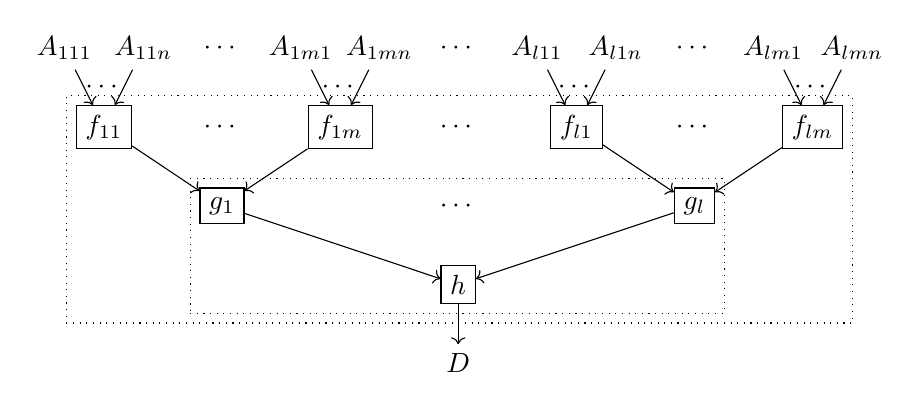
\begin{tikzpicture}
        \path
        % left
        (-5,2) node(A111) {$A_{111}$}
        (-4.5,1.5) node(A1dots) {$\cdots$}
        (-4,2) node(A11n) {$A_{11n}$}
        (-3,2) node(Adots) {$\cdots$}
        (-2,2) node(A1m1) {$A_{1m1}$}
        (-1.5,1.5) node(Amdots) {$\cdots$}
        (-1,2) node(A1mn) {$A_{1mn}$}

        (-4.5,1) node[draw](f11) {$f_{11}$}
        (-3,1) node(fdots) {$\cdots$}
        (-1.5,1) node[draw](f1m) {$f_{1m}$}

        (-3,0) node[draw](g1) {$g_1$}

        % right
        (1,2) node(Al11) {$A_{l11}$}
        (1.5,1.5) node(A1dots) {$\cdots$}
        (2,2) node(Al1n) {$A_{l1n}$}
        (3,2) node(Adots) {$\cdots$}
        (4,2) node(Alm1) {$A_{lm1}$}
        (4.5,1.5) node(Amdots) {$\cdots$}
        (5,2) node(Almn) {$A_{lmn}$}

        (1.5,1) node[draw](fl1) {$f_{l1}$}
        (3,1) node(fdots) {$\cdots$}
        (4.5,1) node[draw](flm) {$f_{lm}$}

        (3,0) node[draw](gl) {$g_l$}

        % middle
        (0,2) node {$\cdots$}
        (0,1) node {$\cdots$}
        (0,0) node {$\cdots$}
        (0,-1) node[draw](h) {$h$}
        (0,-2) node(D) {$D$}
        ;

        \node[draw,dotted,fit=(g1) (gl) (h)] (boxi) {};
        \node[draw,dotted,fit=(f11) (f1m) (fl1) (flm) (boxi)] (boxo) {};

        \draw[->] (A111) -- (f11);
        \draw[->] (A11n) -- (f11);
        \draw[->] (A1m1) -- (f1m);
        \draw[->] (A1mn) -- (f1m);
        \draw[->] (f11) -- (g1);
        \draw[->] (f1m) -- (g1);
        \draw[->] (g1) -- (h);

        \draw[->] (Al11) -- (fl1);
        \draw[->] (Al1n) -- (fl1);
        \draw[->] (Alm1) -- (flm);
        \draw[->] (Almn) -- (flm);
        \draw[->] (fl1) -- (gl);
        \draw[->] (flm) -- (gl);
        \draw[->] (gl) -- (h);

        \draw[->] (h) -- (D);
      \end{tikzpicture}
    \end{matrix}
  \end{displaymath}
\end{definition}

Multicategories have been used as a framework for reasoning with multilinear
maps in linear algebra. \todo{Reference?}
We can produce a multicategory where the objects are vector spaces, and the
multimorphisms are multilinear maps.
In this setting, we can give a universal property to the tensor product of
vector spaces.

\begin{definition}[tensor product \& tensor unit]
  Given a multicategory $\C$, a \emph{tensor product} in $\C$ is a function
  ${\otimes} : \obj\C \times \obj\C \to \obj\C$ and for each pair of objects
  $A$ and $B$, a multimorphism ${\otimes} : A, B \to A \otimes B$ such that,
  for any multimorphism $f : A, B \to C$, there is a unique way to factor $f$
  through $\otimes$, as shown below.
  Similarly, a \emph{tensor unit} is an object $I$ of $\C$ and a multimorphism
  $I : \varepsilon \to I$ supporting a nullary unique factorisation.

  \begin{tikzcd}
    A, B \arrow[rd,"f"'] \arrow[r,"\otimes"] & A \otimes B \arrow[d, dashed] \\
    & C
  \end{tikzcd}
  \begin{tikzcd}
    \varepsilon \arrow[rd,"f"'] \arrow[r,"I"] & I \arrow[d, dashed] \\
    & C
  \end{tikzcd}
\end{definition}

As the proliferation of ellipses suggests, the definition of
\emph{multicategory} I gave above is not entirely rigorous.
Indeed, mechanising the multicategory definition in a reasonably usable way is
considered an open problem. \todo{Check that no-one has done it}
However, we \emph{can} achieve a simple and usable definition in the special
case of \emph{Cartesian} multicategories.

Ordinary multicategories are to monoidal categories as Cartesian multicategories
are to Cartesian categories (i.e., categories with all finite products).
Cartesian multicategories can be defined in terms of ordinary multicategories
--- they are multicategories satisfying the usual ``structural rules'' below
and satisfying various coherence conditions on them.

\begin{align*}
  e &: \hom(\Gamma, A, B, \Delta; C) \to \hom(\Gamma, B, A, \Delta; C) \\
  w &: \hom(\Gamma; B) \to \hom(\Gamma, A; B) \\
  c &: \hom(\Gamma, A, A; B) \to \hom(\Gamma, A; B)
\end{align*}

However, we can bypass ordinary multicategories entirely, and give the following
definition inspired by our earlier formulation of intuitionistic logic.
I define Cartesian multicategories in tandem with the category of contexts and
substitutions that a Cartesian multicategory yields.

\begin{definition}
  A \emph{Cartesian multicategory} comprises the following.

  \begin{itemize}
    \item We have a collection of objects $\obj$.
          We call a list of objects a \emph{context}.
    \item For each context $\Gamma$ and object $A$, we have a set of
          (multi)morphisms $\hom(\Gamma; A)$.
          From this, we derive, for any contexts $\Gamma$ and $\Delta$, a set
          of \emph{substitutions}
          $\sub(\Gamma; \Delta) \coloneqq \prod X \in \Delta.~\hom(\Gamma; X)$.
    \item For every $i : A \in \Gamma$, we have an identity morphism
          $\id(i) : \hom(\Gamma; A)$.
          The collection of identity morphisms over $\Gamma$ serves as the
          identity substitution $\id^s : \sub(\Gamma; \Gamma)$.
    \item For substitution $\sigma : \sub(\Gamma; \Delta)$ and morphism
          $f : \hom(\Delta; A)$, we get a composite morphism
          $\sigma ; f : \hom(\Gamma; A)$.
          This allows us to compose substitutions; for
          $\sigma : \sub(\Gamma; \Delta)$ and $\tau : \sub(\Delta; \Theta)$,
          let $\sigma;^s \tau \coloneqq \lambda k.~\sigma; \tau(k)$.
    \item Identity and composition satisfy the following laws.
          \begin{itemize}
            \item $\sigma; \id(i) = \sigma(i)$
            \item $\id^s; f = f$
            \item $(\sigma;^s \tau); f = \sigma; (\tau; f)$
          \end{itemize}
          It is a simple exercise to see that these laws exactly give us the
          category laws of identity and associativity for substitutions.
  \end{itemize}
\end{definition}

The category of contexts and substitutions is furthermore Cartesian, with the
product being given by context concatenation.

  \section{Weighted multicategories}
  Where Cartesian multicategories give semantics to simply typed
$\lambda$-calculus, we want to find a kind of multicategories that give
semantics to $\name$.

  \section{Applications}

\chapter{Semantics in worldly relations}\label{sec:wrel}

\chapter{A framework for usage-restricted calculi}
  \chapter{A framework for usage-restricted calculi}\label{sec:framework}

In \cref{sec:semirings}, we saw how to use parametrisation over a partially
ordered semiring to recreate a range of usage-aware calculi.
However, $\name$, with its fixed set of type formers and syntactic forms, is a
long way from capturing the full range of linear-like programming languages
studied in the literature and required in practice.

In this chapter, I take the framework for typed syntaxes with binding developed
by \citet{AACMM21} and apply the principles we discovered in
\cref{sec:semirings} to yield a framework allowing for semiring-based usage
restrictions on variables.
Syntactically, I claim that this framework ranges over all finitiary
variable-based simply typed semiring-annotated calculi, with justification by
comparison to the framework of \citet{AACMM21} and some novel examples in
\cref{sec:other-syntaxes}.
I also derive analogues to some of the semantic results of \citet{AACMM21},
strengthening them to take advantage of usage restrictions.

The work in this chapter is fully mechanised in Agda, which allows me to be
precise about the various levels of domain-specific languages which appear.
I assume that the reader is familiar with the bunched connectives introduced in
\cref{fig:bunched} and the usage-aware environments of \cref{def:lr-env}.

\section{Syntax}

We take the insights of the previous section and use them to build a
generic framework for posemiring-annotated substructural systems in
Agda. We will first show \emph{descriptions} of systems, which are
comprised of rules that have premises combined using the bunched
combinators. We then show how to construct the Agda data type of
intrinsically well scoped, typed, and resourced terms for any given
system of our framework. We use the prototypical system from
\cref{fig:lr-comb} as a running example. \cref{sec:other-syntaxes}
presents further examples that our framework can express.

We now start to use Agda notation for record and data type
declarations, to emphasise that our framework has been implemented.

\subsection{Descriptions of Systems}

% We capture the form of rules exemplified previously\todo{Previously?} via
% \emph{descriptions} of rules.
% The key to making these descriptions work is that they only allow syntactic
% forms that preserve environments.
% These forms are: absence and multiplicity of subterms with the same usage
% annotations, absence and multiplicity of subterms with summed usage annotations,
% scaling of a subterm, and variable binding.\todo{Switching to Agda}

\paragraph{\AgdaDatatype{Premises}, \AgdaRecord{Rule}s, and \AgdaRecord{System}s.}

A type \AgdaRecord{System} is made up of multiple \AgdaRecord{Rule}s.
Each \AgdaRecord{Rule} comprises a tree of \AgdaDatatype{Premises} and
a type of conclusion. We assume that there is a
$\AgdaBound{Ty} : \AgdaPrimitiveType{Set}$ of types for the system in
scope.

The \AgdaDatatype{Premise} data type describes premises of rules,
using the bunched combinators from the previous section. A single
premise is introduced by the
\AgdaInductiveConstructor{$\langle$\_`$\vdash$\_$\rangle$}
constructor.  This allows binding of additional variables
\AgdaBound{$\Delta$} (with specified types and usage annotations) and
the specification of a conclusion type \AgdaBound{A} for this premise.
The remaining constructors are descriptions for the first-order
bunched connectives, and will be interpreted directly as such, below.

\ExecuteMetaData[\Syntaxtex]{Premises}

A \AgdaRecord{Rule} is a pair of some \AgdaDatatype{Premises} and a
conclusion. We use an infix arrow as a suggestive notation for rules.

\ExecuteMetaData[\Syntaxtex]{Rule}

Finally, a \AgdaRecord{System} consists of a set of rule labels (i.e.,
constructor names), and for each label a decsription of the
corresponding rule. We use $\rhd$ as infix notation for systems to
associate the label set with the rules.

\ExecuteMetaData[\Syntaxtex]{System}

\paragraph{\cref{fig:lr-comb} as a \AgdaRecord{System}.}

As an example, we transcribe the system defined in
\cref{fig:lr-comb} into a description.  We give the set of types of
this system as a data type \AgdaDatatype{Ty} (together with a base
type \AgdaInductiveConstructor{$\iota$}). We assume that there is a
posemiring \AgdaInductiveConstructor{Ann} in scope for the
annotations.There is one label for each instantiation of a logical
rule, but the labels contain no further information about subterms or
restrictions on the context. This will be provided when we associate
labels with \AgdaRecord{Rule}s in a \AgdaRecord{System}.

\noindent
\begin{minipage}[t]{0.5\textwidth}
  \ExecuteMetaData[\PaperExamplestex]{Ty}
  \ExecuteMetaData[\PaperExamplestex]{Side}
\end{minipage}
\begin{minipage}[t]{0.5\textwidth}
  \ExecuteMetaData[\PaperExamplestex]{qlR}
\end{minipage}

To build a system, we associate with each label a rule:

\ExecuteMetaData[\PaperExamplestex]{lR}

Compared to \cref{fig:lr-comb}, modulo the Agda notation, we can see
that the fundamental structure has been preserved: the rules match
one-to-one, and the bunched premises are the same. A major difference
is that we do not include a counterpart to the
\AgdaInductiveConstructor{var} rule in a
\AgdaRecord{System}. Variables are common to all the systems
representable in our framework.

\paragraph{Terms of a \AgdaRecord{System}.}

The next thing we want to do is to build terms in the described type system.
The following definitions are useful for talking about types indexed over
contexts, judgement forms, and judgement forms admitting newly bound variables,
respectively.

\ExecuteMetaData[\Syntaxtex]{OpenFam}

To specify the meaning of descriptions, we assume some \AgdaBound{X} : \AgdaFunction{ExtOpenFam},
% \ExecuteMetaData[\Interpretationtex]{X},
over which we form one layer of syntax, using the function
\AgdaFunction{$\llbracket$\_$\rrbracket$p} that interprets
\AgdaDatatype{Premises} defined below.  The first argument to
\AgdaBound{X} is the new variables bound by this layer of syntax, as
exemplified in the first clause of
\AgdaFunction{$\llbracket$\_$\rrbracket$p}.  The second argument is
the context containing the variables being carried over from the
previous layer.  Notice that this is not, in general, the same as the
context from the previous layer, because the usage annotations may
have been changed by connectives like
\AgdaInductiveConstructor{\_`$*$\_} and
\AgdaInductiveConstructor{\_`$\cdot$\_}.  The third argument is the
type of subterm required.

With the first clause of \AgdaFunction{$\llbracket$\_$\rrbracket$p} explained,
the rest are simply interpretations of premises into bunched combinators.

\ExecuteMetaData[\Interpretationtex]{semp}

The interpretation of a \AgdaRecord{Rule} checks that the rule targets
the desired type and then interprets the rule's premises \AgdaBound{ps}.
Notice that the interpretation of the premises is independent of the conclusion
of the rule, which accounts for the difference in type between
\AgdaFunction{$\llbracket$\_$\rrbracket$p} and
\AgdaFunction{$\llbracket$\_$\rrbracket$r}.

\ExecuteMetaData[\Interpretationtex]{semr}

The interpretation of a \AgdaRecord{System} is to choose a rule label
\AgdaBound{l} from \AgdaBound{L} and interpret the corresponding rule
\AgdaBound{rs}\AgdaSpace{}\AgdaBound{l} in the same context and for the same
conclusion.

\ExecuteMetaData[\Interpretationtex]{sems}

The most obvious way to make such an \AgdaBound{X} is to use some existing
\AgdaFunction{OpenFam} on an extended context.
We defined \AgdaFunction{Scope} to do this: take the new variables
\AgdaBound{$\Delta$}, concatenate them onto the existing context
\AgdaBound{$\Gamma$}, and pass the extended context onto the judgement
\AgdaBound{T}.

\ExecuteMetaData[\Syntaxtex]{Scope}

%{\color{red}(Forward ref: for now, we could have inlined \texttt{Scope}.)}

We use \AgdaFunction{Scope} to deal with new variables in syntax.
Terms resemble the free monad over a layer-of-syntax functor, though
that picture is complicated by variable binding.  A term is either a
variable or a use of a logical rule together with terms for each of
the required subterms. The \AgdaFunction{Size} argument is where we
use sized types to convince Agda that this type is strictly positive.

\ExecuteMetaData[\Termtex]{Term}

Terms defined like this are still quite difficult to write, mainly because of
frequently changing usage contexts and the need for proofs that they all match
up.
We will see how to automate these proofs in \cref{sec:usage-elaborator}.

%Here is an example term, using the \AgdaFunction{$\lambda$R} system.
%First, for ease of writing, we introduce pattern synonyms for each of the
%typing rules we use.

%\ExecuteMetaData[\PaperExamplestex]{patterns}

%Our example term is a function that flips a tagged union wrapped in an
%arbitrarily annotated \emph{bang}.
%Much of the effort in writing such a term goes into writing the various
%relatedness proofs between usage contexts --- observing, for example, that two
%usage contexts sum together to make a third, or that a usage context used for
%a variable is a basis vector.
%We give a method of automating these proofs in \cref{sec:usage-elaborator}.
%\todo{To be clear, we don't actually write this.}

%\ExecuteMetaData[\HeavyItex]{lR-term}

% A layer of syntax supports the following functorial action.

% \ExecuteMetaData[\Maptex]{map-s-type}

\subsection{Other syntaxes and syntactic forms}\label{sec:other-syntaxes}

\paragraph{The system $\mu\tilde\mu$.}
We can encode a usage-annotated version of System $L$/the
$\mu\tilde\mu$-calculus~\cite{CH00} --- a syntax for classical logic --- in
such a way that contexts capture the undistinguished parts of the sequent.
As such, the generic substitution lemma we get in \cref{sec:kits} is the form
of substitution required in standard $\mu\tilde\mu$-calculus metatheory.
Though the $\mu\tilde\mu$-calculus is originally described as a sequent
calculus~\cite{CH00}, we use the techniques of
\citet[p.~12]{herbelin-hab} and \citet{LC06} to present it as a natural
deduction system, thus giving a notion of \emph{variable} to the system.

Unlike the single judgement form of \name{} and standard simply typed
$\lambda$-calculi, the $\mu\tilde\mu$-calculus has three judgement forms:
terms, coterms, and commands.
Read logically, terms and coterms are seen to, respectively, prove and refute
propositions (types), while commands exhibit contradictions.
This means that the abstract \AgdaBound{Ty} in the generic framework is
instantiated to \AgdaDatatype{Conc} (for \emph{conclusion}) as below, with
\AgdaDatatype{Ty} not being exposed directly to the generic framework.
For now, we just consider multiplicative disjunction $\parr$ (\emph{par}) and
negation/duality, beside an uninterpreted base type.
These are enough to exhibit classical behaviour.

\noindent
\begin{minipage}[t]{0.5\textwidth}
  \ExecuteMetaData[\MuMuTildetex]{Ty}
\end{minipage}
\begin{minipage}[t]{0.5\textwidth}
  \ExecuteMetaData[\MuMuTildetex]{Conc}
\end{minipage}

With \AgdaBound{Ty} instantiated as \AgdaDatatype{Conc}, all terms are assigned
\AgdaDatatype{Conc} type, as are all the variables.
No variables are given \AgdaInductiveConstructor{com} type, similar to how in
the bidirectional typing syntax of \citet[p.~25]{AACMM21}, no variables are
given \AgdaInductiveConstructor{Check} type.
How to observe this invariant is covered in the latter paper, so we will not
repeat it here (having not yet seen how to write traverals on terms).

The syntax comprises a \emph{cut} between a term and a coterm of the same type,
the eponymous $\mu$ and $\tilde\mu$ constructs for proof by contradiction, and
then term and coterm (introduction and elimination) forms for negation and
\emph{par}.

\ExecuteMetaData[\MuMuTildetex]{MMT}

%With a collection of pattern synonyms and the machinery from
%\cref{sec:usage-elaborator}, we can write an example term: a function which
%flips the disjuncts of a \emph{par}.

%\ExecuteMetaData[\MuMuTildeTermtex]{patterns}
%\ExecuteMetaData[\MuMuTildeTermtex]{myComm}

\paragraph{Duplicability}
There is one more bunched combinator we have experimented with adding to the
framework:

\[
  \plr{\Box T}\,\grR \coloneqq \Sigma\grRprime.~\plr{\grRprime \leq \grR}
  \times \plr{\grRprime \leq \gr0}
  \times \plr{\grRprime \leq \grRprime + \grRprime}
  \times T\,\grRprime
\]

The idea of $\plr{\Box T}\,\grR$ is to assert that $\grR$, or some refinement
of it, can be both discarded and duplicated indefinitely, and in the
refinement we have a $T$.
We use this combinator to introduce subterms that are used an unknown number of
times, for example the continuations of the eliminator of an inductive type,
or other fixed points.
We can also use it in linear/non-linear style systems~\cite{Benton94} to make
sure linear variables are not available in the intuitionistic fragment.

Adding the $\Box$ combinator is the only thing we have found that requires our
linear maps be functional rather than merely relational.


\section{Semantics}

Given a $\V$-environment $\Gamma \Rightarrow \Delta$, the function
\AgdaFunction{semantics} we define in this section assigns a
$\C$-value in context $\Gamma$ to every term in context $\Delta$,
where $\C$ is an \AgdaFunction{OpenFam} being the carrier of the
semantic interpretation of terms ($\V$ being the semantic
interpretation of variables). Before we can define
\AgdaFunction{semantics}, we need to treat recursion through rules'
premises (\cref{sec:functorial}) and extension of environments when
going under variable binders (\cref{sec:kripke}).
\todo{Maybe split the chapter here. Syntax/semantics}

% Our goal in this section is to define \AgdaFunction{semantics}, a
% recursor that turns a term into a \AgdaBound{$\C$}-value using a
% \AgdaBound{$\V$}-environment, in a type preserving way:\bob{Get rid of
%   ``body'' here}

% \ExecuteMetaData[\Semanticstex]{semantics-type}

% The \AgdaBound{$\V$} and \AgdaBound{$\C$} are \AgdaFunction{OpenFam}s,
% representing the interpretations of variables and terms
% respectively. In \cref{sec:traversal} we will see the data that must
% be provided to make a \AgdaFunction{semantics} for a given
% system. Before that, we must see how to deal with the two complicated
% features of our syntax: the usage annotations (\cref{sec:functorial})
% and variable binding (\cref{sec:kripke}). \todo{fwd ref to where these are used}

\subsection{A layer of syntax is functorial}\label{sec:functorial}

A basic property of the universe of syntaxes we described in \cref{sec:syntax}
is that every syntax supports a functorial action on subterms, realised by the function \AgdaFunction{map-s}.
Its type says that to map a function \AgdaBound{f}
over a layer of syntax, there must be a linear map \AgdaBound{F} relating the
domain and codomain usage contexts, and \AgdaBound{f} should be usable
wherever the domain and codomain usage contexts are similarly related by
\AgdaBound{F}.

\ExecuteMetaData[\Maptex]{map-s-type}

This generality is needed because usage contexts change between
a term and its immediate subterms---they are decomposed according to the bunched connectives used in the rules.
\AgdaBound{X} and \AgdaBound{Y} are \AgdaFunction{ExtOpenFam}s, with
\AgdaBound{$\Theta$} being the context extension for a subterm (i.e., the
variables newly bound in that subterm).
Unlike usage annotations, types in the contexts \AgdaBound{$\gamma$} and \AgdaBound{$\delta$}, and the conclusion types implicit here, are preserved throughout.
This is the essence of the usage annotation based approach---we use traditional techniques for variable binding, with the usage annotations layered on top.

The heart of \AgdaFunction{map-s} is \AgdaFunction{map-p}, which recursively
works through the structure \AgdaBound{ps} of premises of the rule applied,
acting on each subterm it finds.
Here, particularly in the clauses for \AgdaInductiveConstructor{`$\sep$} and
\AgdaInductiveConstructor{`$\cdot$}, we see why it is not enough for the
function on subterms to apply at usage contexts \AgdaBound{P} and \AgdaBound{Q}
--- rather, it also needs to apply at any similarly related \AgdaBound{P$'$}
and \AgdaBound{Q$'$}.
In the case of \AgdaInductiveConstructor{`$\sep$}, we have that
$\grP \leq \grP_M + \grP_N$, with \AgdaBound{M} and \AgdaBound{N} being
collections of subterms in usage contexts $\grP_M$ and $\grP_N$, respectively.
Linearity of \AgdaBound{F} yields $\grQ_M$ and $\grQ_N$ such that
$\grQ \leq \grQ_M + \grQ_N$ and we use \AgdaFunction{map-p} recursively at
$(\grP_M, \grQ_M)$ and $(\grP_N, \grQ_N)$ on \AgdaBound{M} and \AgdaBound{N}.
The cases for \AgdaInductiveConstructor{`$\cdot$} and
\AgdaInductiveConstructor{`$I^*$} are similar, each using a different aspect
of linearity.
In contrast, the cases for \AgdaInductiveConstructor{`$\dot1$} and
\AgdaInductiveConstructor{`$\dot\times$}, which are the only constructors used in fully structural
systems, do not involve any changes in the usage contexts.

\ExecuteMetaData[\Maptex]{map-p}

\subsection{The Kripke function space}\label{sec:kripke}

At this point we introduce a minor generalisation to
\AgdaFunction{OpenFam} and \AgdaFunction{ExtOpenFam}:
\AgdaBound{I}\AgdaSpace{}\AgdaFunction{---OpenFam} and
\AgdaBound{I}\AgdaSpace{}\AgdaFunction{---ExtOpenFam}.  We obtain the
definition of \AgdaBound{I}\AgdaSpace{}\AgdaFunction{---OpenFam} by
replacing the textual occurrence of \AgdaBound{Ty} by the parameter
\AgdaBound{I}.

The definition \AgdaFunction{Kripke}\,$\V$\,$\C$\,$\Delta$ is a kind
of function space that describes a $\C$ value parametrised by
$\Delta$-many additional $\V$s (all correctly typed and usage
annotated). It is used to describe how to go under binders in a
Higher-Order Abstract Syntax style---to go under a binder we must
provide semantic interpretations for all the additional variables:

% When going under binders during a recursion, the context will be extended by some $\Theta$. This means that the current environment must be extended with $\Theta$s-worth of $\V$s

% we need the ability to say that

% Kripke V C is given the extension \Theta

% In \cref{sec:terms}, we defined \AgdaFunction{Scope} to let a
% judgement-indexed family admit context extensions. However, a key
% component of our generic semantic traversal is to make use of the open
% family \AgdaBound{$\V$} of \emph{values}, which are the sort of thing
% we store in an environment.  The definition \AgdaFunction{Kripke}
% gives an alternative to \AgdaFunction{Scope} which interprets the
% newly bound variables via a requirement of $\V$-values rather than
% extra assumptions for the $\C$-computation.

\ExecuteMetaData[\Semanticstex]{Kripke}

\AgdaFunction{Wrap}
is a device that turns any type family into an equivalent type family
that is judgementally injective in its indices, which helps with
Agda's type inference.
It turns the type family into a parametrised
record with a single field \AgdaField{get} whose type is the type in
the body of the $\lambda$-abstraction.
For understanding the meaning of
\AgdaFunction{Kripke}, \AgdaFunction{Wrap} can be ignored.

If $\Delta$ is of the form $\gr{s_1}B_1, \ldots, \gr{s_n}B_n$, then
\ExecuteMetaData[\Snippetstex]{KripkeVCDGA}\ is equivalent to
\ExecuteMetaData[\Snippetstex]{KripkeExpanded}\ by Currying.  That is
to say, the Kripke function is expecting a value for each newly bound
variable, at the multiplicity of its annotation, together with the
resources supporting each of those values. We use the ``magic wand''
function space here to enforce the invariant that the freshly bound
variables have usage annotations that are added to the existing
variables, not shared with them. The use of the
\AgdaFunction{$\Box^r$} modality ensures that we can still use it in
the presence of additional variables introduced by weakening.

\AgdaFunction{Kripke} is functorial in the \AgdaBound{$\C$} argument,
as witnessed by the \AgdaFunction{mapK$\C$} function, which is essentially
post-composition:

\ExecuteMetaData[\Semanticstex]{mapKC}

% is exemplified by the following construct
% \AgdaFunction{reify}, where we weaken \AgdaBound{$\Gamma$} by a $\gr0$ed-out
% version of \AgdaBound{$\Delta$}.
% The \AgdaBound{$\Delta$} then gets filled in by the $\V$-values.

% \bob{Move this para}
% This means that \AgdaBound{A} in the definition of \AgdaFunction{Kripke} has
% type \AgdaBound{I}, rather than specifically \AgdaBound{Ty}.
% We use this generality later in \AgdaFunction{extend}, setting \AgdaBound{I}
% to \AgdaDatatype{Ctx}.

\subsection{Semantic traversal}\label{sec:traversal}

We can now state the data required to implement a traversal assigning
semantics to terms. For open families $\V$ and $\C$, interpreting
variables and terms respectively, we assume that $\V$ is renameable,
that $\V$ is embeddable in $\C$, and that we have an algebra for a
layer of syntax, where bound variables are handled using the Kripke
function space:

% The aim of this subsection is to give an alternative recursion principle for
% terms that incorporates some of the environment-handling seen in the
% implementations of renaming and substitution.
% The rest of this section assumes the following: a renameable open family
% \AgdaBound{$\V$} that embeds into the open family \AgdaBound{$\C$}, and an
% algebra for a layer of syntax at \AgdaBound{$\C$}.

\ExecuteMetaData[\Semanticstex]{Semantics}

%\ExecuteMetaData[\Semanticstex]{Comp}

We mutually define the action \AgdaFunction{semantics} and its lemma
\AgdaFunction{body}.
The purpose of \AgdaFunction{semantics} is to turn a term into a
\AgdaBound{$\C$}-value using a \AgdaBound{$\V$}-environment and the fields of
\AgdaRecord{Semantics}.
Meanwhile, \AgdaFunction{body} does a similar job, but also deals with
newly bound variables.
In particular, \AgdaFunction{body} takes a term in a context extended by
\AgdaBound{$\Theta$}, and produces a Kripke function from
\AgdaBound{$\V$}-values for \AgdaBound{$\Theta$} to \AgdaBound{$\C$}-values.

\ExecuteMetaData[\Semanticstex]{semantics-type}

To implement the new recursor \AgdaFunction{semantics}, we use the standard
recursor, which in one case gives us a variable \AgdaBound{v}, and in the other
gives us a structure of subterms \AgdaBound{M}, each of which is in an extended
context.
To deal with a variable \AgdaBound{v}, we look it
up in the environment \AgdaBound{$\rho$}, then use the
\AgdaField{$\sem{\text{var}}$} field to map the resulting
\AgdaBound{$\V$}-value to a \AgdaBound{$\C$}-value.
To deal with a structure of subterms \AgdaBound{M}, we use the functoriality of
the syntactic structure to consider each subterm separately.
On a subterm, we apply \AgdaFunction{body}, which amounts to a recursive call
to \AgdaFunction{semantics} with an extended environment.
Recall that \AgdaFunction{relocate} (\cref{thm:env-resize}) adjusts the
environment \AgdaBound{$\rho$} to work in the usage contexts of the subterms.

\ExecuteMetaData[\Semanticstex]{semantics}

For \AgdaFunction{body}, we are given a subterm \AgdaBound{M}, to
which we want to apply \AgdaFunction{semantics}.  To do so, we need an
extended version of the initial environment \AgdaBound{$\rho$}. We
express this as the generation of a Kripke function that produces the
extended environment given interpretations of the fresh variables. We
take \AgdaBound{$\rho$}, which is an environment covering
\AgdaBound{$\Delta$}, and \AgdaBound{$\sigma$}, which is an
environment covering \AgdaBound{$\Theta$}, and glue them together
using the inductive rules for generating environments, after having
renamed \AgdaBound{$\rho$} via \cref{thm:env-ren} to make it fit the
new context \AgdaBound{$\Gamma^+$} (intended to be
\ExecuteMetaData[\Snippetstex]{GT}):

\ExecuteMetaData[\Semanticstex]{extend}

% The best we can achieve without identity environments for \AgdaBound{$\V$} is
% a Kripke function returning an extended environment.
To define \AgdaFunction{body}, we use \AgdaFunction{mapK$\C$} to
post-compose the environment extension by the
\AgdaSymbol{$\lambda$}-function taking an extended environment and
acting with it on \AgdaBound{M}.

\ExecuteMetaData[\Semanticstex]{body}

% \todo{FIX} Under the assumption that \AgdaBound{$\V$} is renameable, we can decompose
% \cref{thm:lr-bind} as
% \AgdaFunction{reify}\AgdaSpace{}\AgdaOperator{\AgdaFunction{$\circ$}}%
% \AgdaSpace{}\AgdaFunction{extend}, with \AgdaFunction{extend} defined below.
% We can think of \AgdaFunction{extend} as our best effort to extend an
% environment by \AgdaBound{$\Theta$} without access to an identity environment
% at \AgdaBound{$\Theta$}.


\section{Example semantics}\label{sec:example-semantics}

\subsection{Renaming and substitution}\label{sec:kits}

In an unpublished note, \citet{McBride05} gives a parametrised traversal
yielding homomorphisms of syntax.
The parameters are collected in the record \AgdaRecord{Kit}.
We make a minor change to the original presentation, where instead of our
\AgdaField{ren\textasciicircum{}$\V$} field, \citeauthor{McBride05} has the
field \AgdaField{wk} allowing only context extensions.
As for the other two fields, \AgdaField{vr} allows us to map variables to
$\V$-values, so as to put newly bound variables in environments; and
\AgdaField{tm} allows us to extract terms from $\V$-values, as required when
we use the environment to evaluate a free variable.

\ExecuteMetaData[\Syntactictex]{Kit}

Where \citeauthor{McBride05} gave the traversal explicitly, we go via our
generic semantic traversal.
The first two fields of \AgdaRecord{Semantics} derive directly from fields of
\AgdaRecord{Kit}.
Meanwhile, to handle term constructors, we first \AgdaFunction{reify} to get a
collection of traversed subterms, and then use \AgdaInductiveConstructor{`con}
to assemble these subterms into a similarly shaped syntactic form as we started
with.
The \AgdaField{vr} field is used implicitly in \AgdaFunction{reify}, as it is
used to show that $\V$-identity environments exist.

\ExecuteMetaData[\Syntactictex]{kit-to-sem}

The action of a syntactic traversal on logical rules is basically fixed: we
preserve the logical rule and extend the environment with any newly bound
variables according to \AgdaField{vr}.
Meanwhile, the action on variables is relatively unconstrained: we look up the
variable in the environment to get a $\V$-value, then transform that $\V$-value
into a term using \AgdaField{tm}.

The idea of renaming is that variables replace variables, whereas with
substitution, terms replace variables.
This translates to environments for renaming containing $\sqni$-values
(variables), and environments for substitution containing $\vdash$-values
(terms).

%To implement renaming and substitution for terms, we now just implement
%syntactic kits for variables and terms, respectively.

\ExecuteMetaData[\Syntactictex]{Ren-Kit}

Notice that \AgdaFunction{ren\textasciicircum$\vdash$}, witnessing the fact
that terms are renameable, is a corollary of \AgdaFunction{Ren-Kit}.

\ExecuteMetaData[\Syntactictex]{Sub-Kit}

\subsection{A denotational semantics}

\todo{Introduction}
To abbreviate this section, we use a simplified syntax compared to \name{}.
We allow for an arbitrary family of base types \AgdaBound{BaseTy}, and a single
type former \mbox{\ExecuteMetaData[\WReltex]{rAToB}}, equivalent to
\mbox{\ExecuteMetaData[\PaperExamplestex]{BangrAToB}} from the earlier system.

\ExecuteMetaData[\WReltex]{Ty}

In the term syntax, $\lambda$-abstraction now binds a variable with annotation
\AgdaBound{r}, while application needs to scale its argument by \AgdaBound{r}
(both in accordance with the function type they are acting on).

\ExecuteMetaData[\WReltex]{AnnArr}

In this subsection, we take the usage annotations to be the 4-element variance
posemiring.
\todo{This works for any semiring.}
We establish the property that all terms are monotonic in their free variables.
This monotonicity can be covariant or contravariant (or neither or both)
depending on the annotation of each free variable.
This provides an additional example to those of \citet{AbelBernardy2020}.
\todo{Cite before here.}

We will take semantics of this system into
\emph{worldly relations}~\cite{AbelBernardy2020}.
A worldly relation over a poset of worlds \AgdaBound{W} is a set over which
we have a \AgdaBound{W}-indexed binary relation satisfying a presheaf-like
property with respect to the order on \AgdaBound{W}.

\ExecuteMetaData[\WReltex]{WRel}

\begin{example}
  When \AgdaBound{W} is the 1-element set, a worldly relation is just a set
  equipped with a binary relation.
\end{example}

Morphisms between worldly relations \AgdaBound{R} and \AgdaBound{S} consist of
a mapping between the underlying sets such that that mapping preserves
relatedness from \AgdaBound{R} to \AgdaBound{S}.

\ExecuteMetaData[\WReltex]{WRelMor}

\todo{Define big intersection.}
When the poset of worlds forms a (relational) commutative monoid, such worldly
relations support a symmetric monoidal closed structure.
We reuse the bunched connectives \AgdaRecord{$I^*$}, \AgdaRecord{$\sep$}, and
\AgdaRecord{$\wand$}, now over worlds rather than contexts.

\ExecuteMetaData[\WReltex]{IR}
\ExecuteMetaData[\WReltex]{tensorR}
\ExecuteMetaData[\WReltex]{lollyR}

The final piece of sematics we need is a \emph{bang} operator.
\todo{No instead}
Instead of requiring extra algebraic structure on the worlds, we allow the
semantic \emph{bang} to be an arbitrary annotation-indexed functor on worldly
relations.
This functor must respect all of the structure on the indices, making it a
graded comonad over multiplication, as well as being lax monoidal at any
particular index \AgdaBound{r}.

\ExecuteMetaData[\WReltex]{Bang}

\begin{example}
  With \AgdaBound{W} being the 1-element set and annotations coming from the
  variance semiring, we can define the following \emph{bang}.
  It is always the identity on the set component, while the relation component
  consists of flipping the relation for contravariance and taking conjunctions
  to achieve both covariance and contravariance.
  When we want neither covariance nor contravariance, we use the always true
  predicate on worlds \AgdaFunction{$\dot1$}.

  \ExecuteMetaData[\Monotonicitytex]{BangR}
\end{example}

To associate semantics to syntax, we start as standard by associating worldly
relations to types.
We also extend the semantics of types to contexts, using \AgdaFunction{I$^R$},
\AgdaFunction{$\otimes^R$}, and \AgdaField{!$^R$} to interpret the empty
context, concatenation, and usage annotations on singletons, respectively.

\ExecuteMetaData[\WReltex]{sem}

The semantics of a term is then to be a morphism from the interpretation of the
context to the interpretation of the term's type.

\ExecuteMetaData[\WReltex]{sem-vdash}

Variables are given semantics by \AgdaFunction{lookup$^R$} (definition omitted).

\ExecuteMetaData[\WReltex]{lookupR-type}

Now, we give a \AgdaRecord{Semantics}.
The choice of \AgdaBound{$\V$} as
\AgdaRecord{\AgdaUnderscore{}$\sqni$\AgdaUnderscore{}} is somewhat arbitrary,
given that a standard denotational semantics would not use intermediate
environments in the same sense as renaming and substitution, but allows us to
reuse the standard facts that variables support renaming and identity
environments.
With this choice of \AgdaBound{$\V$} and \AgdaBound{$\C$}, we interpret
environment entries by \AgdaFunction{lookup$^R$}.
Meanwhile, for the logical rules, we ignore environments by using
\AgdaFunction{reify} to just deal with morphisms in an extended context.
As such, $\lambda$-abstractions are easy to interpret, while applications
require some massaging to remove the extension by an empty context, followed by
some plumbing to split the interpretation of the context according to the usage
constraints and feed the interpretation of the argument \AgdaBound{n$'$} into
the interpretation of the function \AgdaBound{m$'$}.

\ExecuteMetaData[\WReltex]{Wrel}

In order to map open terms to interpretations, we take the action of the
semantics and give the identity renaming as the starting environment.

\ExecuteMetaData[\WReltex]{wrel}

\begin{example}
  We can make a subtraction function from primitive addition and negation on
  integers.
  Subtraction is covariant in its first argument and contravariant in its
  second argument.
  We give the definition in pseudocode, as we have not yet seen how to
  conveniently write terms (\cref{sec:usage-elaborator}).

  \begin{align*}
    &{\sim\sim}p :
      {\uparrow\uparrow}\mathbb Z \multimap
      {\uparrow\uparrow}\mathbb Z \multimap \mathbb Z,
      {\sim\sim}n : {\downarrow\downarrow}\mathbb Z \multimap \mathbb Z
      \vdash \mathnormal{minus} :
      {\uparrow\uparrow}\mathbb Z \multimap
      {\downarrow\downarrow}\mathbb Z \multimap
      \mathbb Z
    \\
    &\mathnormal{minus} \coloneqq \lambda x.~\lambda y.~p\,x\,(n\,y)
  \end{align*}

  We observe that the set component of this term's semantics is just the
  expected Agda function when the two free variables are given appropriate
  interpretations.

  \ExecuteMetaData[\Monotonicitytex]{minus-set}

  Furthermore, the relational component of the semantics yields the free
  theorem that the Agda subtraction so defined is monotonic in the expected way.
  This relies on library proofs that addition and negation are suitably
  monotonic.

  \ExecuteMetaData[\Monotonicitytex]{thm}
\end{example}

\subsection{A usage elaborator}\label{sec:usage-elaborator}

Using the constructs we have seen so far, producing example terms soon becomes
extremely tedious.
We achieved some abbreviation by using pattern synonyms, but we still have to
produce essentially bespoke proofs whenever we use a usage-sensitive part of the
syntax.
The size of each of these proofs is roughly proportional to the number of free
variables, so the amount of proof we have to write grows roughly quadratically
with the size of terms.
An additional factor, which we can't see on paper, is that type checking time
for these proofs soon becomes prohibitive to interactive development.

Our aim in this subsection is to automate usage constraint proofs, making terms
both easier to write and more performant to check.
We invoke the automation by writing terms in a syntax where usage constraints
have been trivialised, and then use a semantic traversal over the simplified
syntax to try to produce a fully elaborated term in the original syntax.
We write the automation in a way that is generic in the syntax description, thus
avoiding repetition and facilitating the prototyping of new type systems.

The type of syntax descriptions depends on the type of usage annotations because
of variable binding.
For example, in the $\oc_{\gr r}$-E rule of \cref{fig:lr-comb}, the right
premise binds a new variable with annotation $\gr r$, where $\gr r$ is drawn
from the ambient posemiring.
The scaling combinator also makes direct reference to the posemiring.
To produce a simplified syntax description, where usage constraints are
trivialised, we set the ambient posemiring to the 1-element $\mathbf0$
posemiring.
In contrast to syntax descriptions, even though types can contain usage
annotations, the type of types does not depend on the type of usage annotations.
This means that, in our simplified syntax, terms have types from the original
system even though variables have trivial usage annotations.
We define the $\mathbf0$ posemiring as follows, being careful to use the
0-field record type \AgdaRecord{$\top$} so that everything algebraic gets
solved by Agda's $\eta$-laws.
Indeed, in this very definition, all of the semiring operations and laws are
canonically inferred.

\ExecuteMetaData[\UsageChecktex]{0-poSemiring}

The elaboration process is monadic.
In particular, we use the \AgdaDatatype{List}/non-determinism monad to give
\emph{all} of the possible annotation choices on the free variables of a term.
We believe the commitment to multiple solutions is inherent when the syntax
contains \AgdaInductiveConstructor{`$\dot1$}.
For example, in the intermediate stages of elaborating
$\plr{\vdash \lambda x.~\plr{*,*}} : A \multimap \top \otimes \top$ with a
usage counting posemiring (assuming reasonable rules for $\top$ and $\otimes$),
it is unclear whether to use the variable $x$ in the left $*$ or the right $*$.
This uncertainty should be reflected in the final result.

The non-deterministic choices we make during elaboration are enumerated by
the fields of \AgdaRecord{NonDetInverses}.
These choices are driven by the typing rules and a candidate usage vector for
the conclusion.
For example, \AgdaField{+$^{-1}$}\AgdaSpace{}\AgdaBound{r} is needed when we
encounter a \AgdaInductiveConstructor{`$\sep$} in the syntax and the candidate
usage annotation we are considering is \AgdaBound{r}.
Then, \AgdaField{+$^{-1}$}\AgdaSpace{}\AgdaBound{r} is a list of pairs of
annotations \AgdaBound{p} and \AgdaBound{q} that \AgdaBound{r} can split into,
together with a proof of the splitting.
For \AgdaField{0\#$^{-1}$} and \AgdaField{1\#$^{-1}$}, inverses to constants,
we are given the candidate \AgdaBound{r} and typically return an empty list if
the constraint cannot be satisfied, or a singleton list containing a proof.
\AgdaField{*$^{-1}$} is used when we encounter scaling, in which case we know
both the scaling factor \AgdaBound{r} (from the syntax description) and the
candidate \AgdaBound{q}.
These inverse operations combine monadically (in fact, applicatively) to give
inverses to the vector operations of zero, addition, scaling, and basis.

\ExecuteMetaData[\UsageChecktex]{NonDetInverses}

We choose the \AgdaBound{$\V$} of our semantics to be (unannotated) variables.
For the \AgdaBound{$\C$}, we consider \emph{functions} from candidate usage
vectors \AgdaBound{R} to the list of elaborated derivations with usage
annotations given by \AgdaBound{R}.
The module name \AgdaModule{U} refers to the fact that we are taking the
ambient posemiring to be $\mathbf0$ in \AgdaFunction{OpenFam}.
The effect on \AgdaFunction{OpenFam} is that the usage annotations of any
contexts we consider are uninformative (hence the \AgdaSymbol{\_} on the left).

\ExecuteMetaData[\UsageChecktex]{C}

To traverse the unannotated terms, we produce a \AgdaRecord{Semantics} over the
unannotated system \AgdaFunction{uSystem}\AgdaSpace{}\AgdaBound{sys}.
We already know that variables are renameable.
To interpret a variable, we consider all the possible proofs that such a
variable could be well annotated, and package them up as a variable term.

\ExecuteMetaData[\UsageChecktex]{elab-sem}

\ExecuteMetaData[\UsageChecktex]{lemma-type}

To actually use \AgdaFunction{elab-sem} on terms, we take the associated
\AgdaFunction{semantics} and pass it the identity environment (an identity
\emph{renaming} in this case, because $\V$ is a family of variables).
The candidate usage vector \AgdaBound{R} will be empty for closed terms, and
otherwise we have to supply the intended usage annotations.



\chapter{Generic programs}
  \section{Usage checker}

\chapter{Investigations that are now easier}
  \section{Linear/non-linear logic}
  In \cref{sec:dup-lnl}, I gave what I claimed to be an encoding of
Linear/non-Linear logic~\citep{Benton94} as a syntax description.
In this section, I rigorously state and prove the correspondence between
\citeauthor{Benton94}'s definition of L/nL and my encoding of it.
Then, I give translations from this encoding to my encoding of $\name$, and
vice versa, using two generic semantic traversals.
These results together should give us confidence that the encoding of L/nL is
correct up to logical equivalence.

\subsection{Encoding L/nL}\label{sec:encoding-LnL}

I will present translations between the systems given by
\cref{fig:LnL-orig,fig:LnL-bunched}.

I use $S$ to range over both linear and intuitionistic variables.
In this section, I use the notations $\Gamma \vdash A$ and $\Gamma \vdash X$
without subscripts on the turnstile to refer to the encoded version of the
calculus.
This notation keeps the encoded calculus distinct from the reference L/nL
calculus I am translating from and to.

The main difference between the original L/nL calculus and the encoded version
is that the encoded version contains some extra ``junk'', not corresponding to
anything in the original L/nL calculus.
This junk includes all of the wrinkles we saw when translating to and from DILL
in \cref{sec:trans-dill} --- where in the semiring-annotated system, variables
annotated $\gr\omega$ (corresponding to intuitionistic variables) can slip into
having annotation $\gr1$ or $\gr0$ whenever there are any algebraic
manipulations of the context.
In linear/non-linear logic, this slipping causes extra problems because
intuitionistic variables are supposed to be of a distinct sort to other
(i.e., linear) variables.
Additionally, we have no means in the framework to correlate types with usage
annotations, so we must deal with free variables carefully to ensure the
required correlation between linear and intuitionistic types and annotations.

With the above remarks in mind, I take it as clear how to translate the original
L/nL calculus into the encoded version, and just state the type of the
translation in \cref{thm:lnl-to-enc} without including a proof.
In contrast, I spend most of this subsection on the reverse translation, which
I provide a proof sketch of in \cref{thm:enc-to-lnl}.

\begin{proposition}\label{thm:lnl-to-enc}
  We can construct the following translations.
  \begin{align}
    (\Theta \vdashC X) &\to (\gr\omega\Theta \vdash X) \\
    (\Theta; \Gamma \vdashL A) &\to (\gr\omega\Theta, \gr1\Gamma \vdash A)
  \end{align}
\end{proposition}

The key property needed to sensibly do the reverse translation is
\emph{linear well-formedness}, as given by \cref{def:lin-well-formed}.
Linear well-formedness says that variables of linear type have linear usage
annotations.
It does not say anything about intuitionistic types and usage annotations for
two reasons.
First, talking about $\gr\omega$ is not sufficiently stable.
As we work up a derivation, the ``slip'' described earlier says that usage
annotations will tend to get larger, i.e.\ more precise.
Therefore, it makes more sense to make conditions of being greater than or equal
to some collection of usage annotations.
Second, it turns out to be unnecessary to add any conditions on variables with
intuitionistic type, because we can just treat them as if they were annotated
$\gr\omega$.
We can forget the specificness of annotations $\gr0$ and $\gr1$ when not needed,
because whatever a specifically annotated variable can do can be done by an
$\gr\omega$-annotated variable.

\begin{definition}\label{def:lin-well-formed}
  A semiring-annotated context for L/nL is \emph{linearly well formed} when all
  linear variables are annotated either $\gr0$ or $\gr1$.
\end{definition}

\begin{lemma}\label{thm:lwf}
  If $\Gamma$ is linearly well formed and $M : \plr{\Gamma \vdash S}$, then the
  context of every subterm of $M$ is linearly well formed.
\end{lemma}
\begin{proof}
  This lemma follows by inspection of the syntax description
  (\cref{fig:LnL-bunched}).
  In the subterms, the linear variables in $\Gamma$ are only changed by binding
  new variables (all instances of which maintain linear well formedness) and by
  existing variables being shared out or coerced (which never produces
  $\gr\omega$ annotations from $\gr0$ or $\gr1$).
\end{proof}

Linear well-formedness is the only condition needed for the translation given by
\cref{thm:enc-to-lnl}.
We can translate a derivation with any such context, with no further
specification of its shape.
In particular, the shape is not calculated from an original L/nL context.

\begin{proposition}\label{thm:enc-to-lnl}
  Let $\Gamma_{\mathcal C}$ be the list of variables of intuitionistic type in
  $\Gamma$.
  Let $\Gamma_{\mathcal L}$ be the list of variables of linear type in $\Gamma$
  with usage annotation $\gr1$.
  Then, whenever $\Gamma$ is linearly well formed, we can construct the
  following translations.
  \begin{align}
    (\Gamma \vdash X) &\to \plr{\Gamma_{\mathcal C} \vdashC X} \\
    (\Gamma \vdash A) &\to
      \plr{\Gamma_{\mathcal C}; \Gamma_{\mathcal L} \vdashL A}
  \end{align}
\end{proposition}
\begin{proof}
  We proceed by mutual induction on the derivations.

  First, I consider variables.
  Suppose we have $\Gamma \sqni S$.
  If $S$ is a linear type $A$, then $\Gamma$ contains one variable of type $A$
  annotated $\gr1$, while all of the other linear variables are annotated $\gr0$
  (by linear well formedness, we have no linear variables annotated
  $\gr\omega$).
  Therefore, $\Gamma_{\mathcal L} = A$, and \TirName{$\mathcal L$-var} applies.
  Otherwise, if $S$ is an intuitionistic type $X$, then
  \TirName{$\mathcal C$-var} applies to yield $\Gamma_{\mathcal C} \vdashC X$.

  For the logical rules, linear well formedness means that all variables of
  linear type act linearly.
  Additionally, every L/nL rule requiring there to be no linear variables in
  scope is guarded by $\Boxzpt$ or $I^*$ in the syntax description, excluding
  linear variables.
  Given these behaviours, the two calculi correspond closely, and it is a matter
  of inspection (and use of \cref{thm:lwf} when using the induction hypothesis)
  to complete the proof.
\end{proof}

\subsection{Translating between L/nL and $\lambda\gr{\mathcal R}$}

\Citet[\S 3.3]{Benton94} gives syntactic translations back and forth between
Linear/non-Linear logic and the presentation of intuitionistic linear logic
given by \citet{BBdePH93}.
In this section, I give analogous translations between my encodings of L/nL and
$\name$ as instances of the generic traversal \AgdaFunction{semantics}.
More precisely, I instantiate $\name$ to the $\{\gr0 > \gr\omega < \gr1\}$
posemiring and restrict it to the fragment containing connectives $I$,
$\otimes$, $\multimap$, and $\oc\gr\omega$, matching the fragment of L/nL
presented by \citeauthor{Benton94} and in this section.
Notably, this fragment of $\name$ excludes $\oc\gr0$ and $\oc\gr1$.
I write $\oc\gr\omega$ as just $\oc$, as in traditional linear logic.

Under the above restrictions and conventions, \citeauthor{Benton94}'s
translations between the types of ILL and L/nL can be used verbatim,
and are reproduced in \cref{fig:lnl-lr-types}.
Notably, the image of each ILL type under the $\plr{-}^o$-translation falls in
the \emph{linear} types of L/nL.
In the other direction (the $\plr{-}^*$-translation), we make extensive use of
the $\oc$-type former to translate the intuitionistic types of L/nL.

\begin{figure}
  \centering
  \begin{subfigure}{.49\linewidth}
    \centering
    \begin{align*}
      &(-)^* : \mathrm{Ty}_\lnl \to \mathrm{Ty}_{\name} \\
      &\begin{aligned}
        I^* &= I \\
        \plr{A \otimes B}^* &= A^* \otimes B^* \\
        \plr{A \multimap B}^* &= A^* \multimap B^* \\
        \plr{FX}^* &= \oc X^* \\
        1^* &= I \\
        \plr{X \times Y}^* &= \oc X^* \otimes \oc Y^* \\
        \plr{X \to Y}^* &= \oc X^* \multimap Y^* \\
        \plr{GA}^* &= A^*
      \end{aligned}
    \end{align*}
    \begin{align*}
      &(-)^* : \mathrm{Ctx}_\lnl \to \mathrm{Ctx}_{\name} \\
      &\plr{\plr{\grR\gamma}^*}_i = \grR_i\gamma_i^*
    \end{align*}
  \end{subfigure}
  \begin{subfigure}{.49\linewidth}
    \centering
    \begin{align*}
      &(-)^\circ : \mathrm{Ty}_{\name} \to \mathrm{Ty}_{\lin} \\
      &\begin{aligned}
        I^\circ &= I \\
        \plr{A \otimes B}^\circ &= A^\circ \otimes B^\circ \\
        \plr{A \multimap B}^\circ &= A^\circ \multimap B^\circ \\
        \plr{\oc A}^\circ &= GFA^\circ
      \end{aligned}
    \end{align*}
    \begin{align*}
      &(-)^\circ : \oiw \times \mathrm{Ty}_{\name} \to \Sigma_f~\mathrm{Ty}_f \\
      &\begin{aligned}
        \plr{\gr0A}^\circ &= \plr{\lin, A^\circ} \\
        \plr{\gr1A}^\circ &= \plr{\lin, A^\circ} \\
        \plr{\gr\omega A}^\circ &= \plr{\intu, GA^\circ}
      \end{aligned}
    \end{align*}
    \begin{align*}
      &(-)^\circ : \mathrm{Ctx}_{\name} \to \mathrm{Ctx}_\lnl \\
      &\plr{\plr{\grR\gamma}^\circ}_i = \grR_i\plr{\grR_i\gamma_i}^\circ
    \end{align*}
  \end{subfigure}
  \caption{Translation of types between L/nL and $\name$}
  \label{fig:lnl-lr-types}
\end{figure}

I extend $\plr{-}^*$ to contexts pointwise on the type context.
Note that this differs from \citeauthor{Benton94}'s translation of contexts in
that the intuitionistic variables of $\lnl$ are translated using usage
annotation $\gr\omega$, rather than type former $\oc$.
A translation from $\lnl$ to DILL would probably similarly use DILL's
intuitionistic variables rather than $\oc$.

For $\plr{-}^\circ$, I use an extra step to avoid producing contexts
that are not linearly well formed per \cref{def:lin-well-formed}.
Specifically, wherever there is an annotation $\gr\omega$ in a $\name$ context,
the corresponding type is wrapped in a $G$ to make it intuitionistic.
For example, $\plr{\gr0A, \gr1B, \gr\omega C}^\circ =
\plr{\gr0A^\circ, \gr1B^\circ, \gr\omega GC^\circ}$.

In Agda code, I define the $\plr{-}^\circ$ operator on
$\oiw \times \mathrm{Ty}_{\name}$ (the one that introduces a $G$ for each
$\gr\omega$) via a \emph{view} \AgdaDatatype{LIView}~\citep{MM04}.
I define usage annotations $\gr0$ and $\gr1$ (\AgdaInductiveConstructor{0\#} and
\AgdaInductiveConstructor{1\#} in Agda) to be \emph{linear}, with only
$\gr\omega$ (\AgdaInductiveConstructor{$\upomega$\#}) being
\emph{intuitionistic}.
\AgdaDatatype{LIView} is a view because of the existence of
\ExecuteMetaData[\LinIntViewtex]{liview-type}, and well behaved in the sense
that any two views of the same usage annotation are equal (witnessed by
\AgdaFunction{liview-prop}, not shown here).
The translation from $\name$ to $\lnl$ takes cases between linear and non-linear
annotations at many points, so having these cases expressed as a view avoids
duplication of arguments between the cases for $\gr0$ and $\gr1$.

\ExecuteMetaData[\LinIntViewtex]{Linear}
\ExecuteMetaData[\LinIntViewtex]{LIView}

\begin{theorem}\label{thm:lnl-to-lr}
  Let $S$ be an $\lnl$ type, either linear or intuitionistic.
  Then, we can translate any L/nL term to a $\name$ term as follows.
  \begin{align}
    (\Gamma \vdash_\lnl S) &\to (\Gamma^* \vdash_{\name} S^*)
  \end{align}
\end{theorem}
\begin{proof}
  The proof is mostly straightforward, largely following Benton's translation.
  Similarly to the denotational semantics of \cref{sec:den-sem}, we may use a
  \AgdaRecord{Semantics} with $\V$ set to $\sqni_{\lnl}$, and then set
  $\C\,\Gamma\,S \coloneqq \Gamma^* \vdash_{\name} S^*$.
  Whenever we have induction hypotheses of \AgdaFunction{Kripke} type, we use
  the \AgdaFunction{reify} function for $\name$ to get $\name$ terms.
  Therefore, we are essentially just doing a proof by induction on the structure
  of the input term.

  Translating the \TirName{$F$i} rule into \TirName{$\oc$i} relies
  on the equivalence between duplicability (as expressed by the $\Box$ premise
  connective) and having been scaled by $\gr\omega$ (as expressed by the
  $\gr\omega \cdot {}$ premise connective).
  This holds of the $\oiw$ semiring, but not of general semirings (and is not
  even stateable for general semirings because of the mention of $\gr\omega$).
  The same reasoning is needed when translating the introduction rules for
  intuitionistic connectives, because they always have $\Box$ed premises and
  are translated using $\oc$.

  As an example of translating an intuitionistic elimination rule, let us
  consider the \TirName{$\times$e$_0$} rule.
  I reproduce it here with explicit contexts.
  \[
    \ebrule{%
      \hypo{\Gamma' \leq \Gamma}
      \hypo{\Gamma\text{ duplicable}}
      \hypo{\Gamma \vdash_{\lnl} X \times Y}
      \infer3[$\times$e$_0$]{\Gamma' \vdash_{\lnl} X}
    }
  \]

  Recall that $\plr{X \times Y}^* = \oc X^* \otimes \oc Y^*$.
  This means that we must pattern-match the hypothesis to get variables
  $\gr\omega X^*, \gr\omega Y^*$ so as to be able to use the $X^*$ for the
  conclusion and discard the $Y^*$.
  The formal derivation is as follows.
  We are able to copy $\Gamma^*$ between all of these subterms because its usage
  annotations are the same as those of $\Gamma$, which is duplicable by the
  assumption in \TirName{$\times$e$_0$}.
  The distinction between $\Gamma'$ and $\Gamma$ is minor.
  When we apply the \TirName{$\otimes$e} rule, we use the fact that
  $\Gamma' \leq \Gamma + \Gamma$, by the fact that $\Gamma' \leq \Gamma$ and
  $\Gamma \leq \Gamma + \Gamma$.
  From then on, we need only think about $\Gamma$, which behaves well because it
  is duplicable.

  \begin{align*}
    &\ebrule{%
      \hypo{\text{IH}}
      \infer[no rule]1{\Gamma^* \vdash_{\name} \oc X^* \otimes \oc Y^*}
      \infer0[Var]{\Gamma^*, \gr1\oc X^*, \gr0\oc Y^* \vdash_{\name} \oc X^*}
      \hypo{\nabla}
      \infer2[$\oc$e]{\Gamma^*, \gr1\oc X^*, \gr1\oc Y^* \vdash_{\name} X^*}
      \infer2[$\otimes$e]{\Gamma^* \vdash_{\name} X^*}
    }
    \\
    &\text{where }\nabla \coloneqq
    \\
    &\ebrule{%
      \infer0[Var]{\Gamma^*, \gr0\oc X^*, \gr1\oc Y^*, \gr\omega X^* \vdash_{\name} \oc Y^*}
      \infer0[Var]{\Gamma^*, \gr0\oc X^*, \gr0\oc Y^*, \gr\omega X^*, \gr\omega Y^* \vdash_{\name} X^*}
      \infer2[$\oc$e]{\Gamma'^*, \gr0\oc X^*, \gr1\oc Y^*, \gr\omega X^* \vdash_{\name} X^*}
    }
  \end{align*}

  In the Agda proof, renaming is required to perform lots of minor functions
  that we would ignore on paper.
  For example, the equation $\plr{\Gamma, \Delta}^* = \Gamma^*, \Delta^*$ ---
  required when induction hypotheses have newly bound variables --- is not true
  definitionally.
  Furthermore, because of the functional representation I use for contexts, it
  is not even provable without function extensionality.
  Therefore, renaming is the simplest way to get the required coercion.
  Such renamings perhaps could be avoided in most cases if contexts were
  represented as non-functional lists.
\end{proof}

\begin{theorem}\label{thm:lr-to-lnl}
  We can translate from $\name$ to the linear fragment of $\lnl$.
  \begin{align}
    (\Gamma \vdash_{\name} A) \to (\Gamma^\circ \vdash_\lnl A^\circ)
  \end{align}
\end{theorem}
\begin{proof}
  We use the same simple induction scheme as in \cref{thm:lnl-to-lr}, but with
  the places of $\name$ and $\lnl$ switched.
  However, some of the rule translations are more complex, mainly caused by the
  complexity of the $\plr{-}^\circ$ translation on contexts.

  For variables, we must consider separately the cases where the variable being
  used is annotated $\gr1$ and $\gr\omega$.
  The case for a variable $\gr1A$ is straightforward, and translates directly
  to an $\lnl$ variable $\gr1A^\circ$.
  A variable $\gr\omega A$, however, is translated to $\gr\omega GA^\circ$, so
  we must eliminate the $G$ in order to get the conclusion $A^\circ$.
  The \TirName{$G$e} rule requires its context to be duplicable, which is true
  by the fact that all of the unused variables are annotated either $\gr0$ or
  $\gr\omega$ (because they are all less than or equal to $\gr0$), and the
  variable being used is annotated $\gr\omega$.

  Most logical rules are handled very similarly to each other, so I will just
  translate the \TirName{$\otimes$i} rule as an example.
  I reproduce it here with explicit contexts (split into their usage and typing
  contexts).

  \[
    \ebrule{%
      \hypo{\grR \leq \grP + \grQ}
      \hypo{\grP\gamma \vdash_{\name} A}
      \hypo{\grQ\gamma \vdash_{\name} B}
      \infer3[$\otimes$i]{\grR\gamma \vdash_{\name} A \otimes B}
    }
  \]

  We cannot do a na\"{i}ve translation to the corresponding application of the
  \TirName{$\otimes$i} rule of $\lnl$ because $\plr{\grR\gamma}^\circ$,
  $\plr{\grP\gamma}^\circ$, and $\plr{\grQ\gamma}^\circ$ may all have different
  typing contexts.
  For example, consider the following instance.
  There are two problems.
  First, our induction hypotheses give us contexts
  containing $C^\circ$, where our conclusion wants a context containing
  $GC^\circ$.
  Second, $\gr1GC^\circ$ is not linearly well formed, because an intuitionistic
  type is given a linear annotation.
  It is therefore difficult to work with such a sequent.

  \[
    \ebrule{%
      \hypo{\gr1 C \vdash_{\name} A}
      \hypo{\gr1 C \vdash_{\name} B}
      \infer2[$\otimes$i]{\gr\omega C \vdash_{\name} A \otimes B}
    }
    \quad\rightsquigarrow\quad
    \ebrule{%
      \hypo{\gr1C^\circ \vdash_{\lnl} A^\circ}
      \ellipsis{?}{\gr1 GC^\circ \vdash_{\lnl} A^\circ}
      \hypo{\gr1C^\circ \vdash_{\lnl} B^\circ}
      \ellipsis{?}{\gr1 GC^\circ \vdash_{\lnl} B^\circ}
      \infer2[$\otimes$i]{\gr\omega GC^\circ \vdash_{\lnl} A^\circ \otimes B^\circ}
    }
  \]

  To fix these issues, firstly I overwrite the context-splitting given by the
  input term to conform to the bottom-up style of \cref{def:DILL-bottom-up}.
  This means precisely that wherever $\gr\omega$ appears in the context of the
  conclusion, it will also appear in the context of all the hypotheses.
  This gives the following partial derivation.

  \[
    \ebrule{%
      \hypo{\gr1C^\circ \vdash_{\lnl} A^\circ}
      \ellipsis{?}{\gr\omega GC^\circ \vdash_{\lnl} A^\circ}
      \hypo{\gr1C^\circ \vdash_{\lnl} B^\circ}
      \ellipsis{?}{\gr\omega GC^\circ \vdash_{\lnl} B^\circ}
      \infer2[$\otimes$i]{\gr\omega GC^\circ \vdash_{\lnl} A^\circ \otimes B^\circ}
    }
  \]

  Then, I fix the discrepancy in types using substitution.
  In the running example, the substitution needed for both subterms is of the
  type $\gr\omega GC^\circ \env{\vdash_{\lnl}} \gr1C^\circ$, which amounts to a
  term of type $\gr\omega GC^\circ \vdash_{\lnl} C^\circ$, as follows.
  Note that \TirName{$G$e} is only applicable thanks to changing the usage
  annotation from $\gr1$ to $\gr\omega$ in the previous step.

  \[
    \ebrule{%
      \infer0[Var]{\gr\omega GC^\circ \vdash_{\lnl} GC^\circ}
      \infer1[$G$e]{\gr\omega GC^\circ \vdash_{\lnl} C^\circ}
    }
  \]

  More generally, we may have to produce substitutions of type
  $$\gr0A^\circ, \gr1B^\circ, \gr\omega GC^\circ, \gr\omega GD^\circ
  \env{\vdash_{\lnl}}
  \gr0A^\circ, \gr1B^\circ, \gr1C^\circ, \gr\omega GD^\circ.$$
  These can be produced pointwise, from substitutions of types
  $\gr0A^\circ \env{\vdash_{\lnl}} \gr0A^\circ$ and
  $\gr1B^\circ \env{\vdash_{\lnl}} \gr1B^\circ$ and
  $\gr\omega GC^\circ \env{\vdash_{\lnl}} \gr1C^\circ$ and
  $\gr\omega GD^\circ \env{\vdash_{\lnl}} \gr\omega GD^\circ$.
  We have just seen how to produce the third of these, and the rest are
  identity substitutions.

  The two sui generis rules to translate are the rules for the $\oc$-modality,
  with the $\oc$ of intuitionistic linear logic becoming the composite $FG$ in
  linear/non-linear logic.
  The way of handling \TirName{$\oc$i} is similar to the way of handling rules
  like \TirName{$\otimes$i}, but involving multiplication/scaling by $\gr\omega$
  rather than addition.
  We have a similar difficult instance, shown below, where an $\gr\omega$ gets
  specialised to a $\gr1$ via the algebraic operation.

  \[
    \ebrule{%
      \hypo{\gr\omega \leq \gr\omega \cdot \gr1}
      \hypo{\gr1 C \vdash_{\name} A}
      \infer2[$\oc$i]{\gr\omega C \vdash_{\name} \oc A}
    }
  \]

  Again, the solution is to fix up the operation to keep the more general
  $\gr\omega$, allowing us to apply \TirName{$F$i} and \TirName{$G$i}, and
  the same substitution as before possibly including an application of
  \TirName{$G$e} as necessary.

  Finally, the translation of \TirName{$\oc$e} is simple, but worth checking.
  I reproduce the rule below with explicit contexts.

  \[
    \ebrule{%
      \hypo{\grR \leq \grP + \grQ}
      \hypo{\grP\gamma \vdash_{\name} \oc A}
      \hypo{\grQ\gamma, \gr\omega A \vdash_{\name} B}
      \infer3[$\oc$e]{\grR\gamma \vdash_{\name} B}
    }
  \]

  The main thing to note is that the translation of the context of the
  right-hand premise, $\grQ\gamma, \gr\omega A$, is
  $\plr{\grQ\gamma}^\circ, \gr\omega GA^\circ$ --- i.e., the translation of
  contexts gives us a $G$ thanks to the $\gr\omega$ usage annotation.
  Therefore, we do not have to eliminate the $G$, because the right-hand subterm
  is expected to do it for us.
  Indeed, we have seen in previous cases many uses of \TirName{$G$e} already.

  I translate the \TirName{$\oc$e} rule as follows.
  As in the \TirName{$\otimes$i} case, I pick $\grPprime$ and $\grQprime$ to fit
  bottom-up form, and use the same substitutions as in that case to mend the
  terms arriving from the induction hypotheses.
  Then, just \TirName{$F$e} suffices.

  \[
    \ebrule{%
      \infer0{\grR \leq \grPprime + \grQprime}
      \hypo{}
      \ellipsis{}{\plr{\grPprime\gamma}^\circ \vdash_{\lnl} FGA^\circ}
      \hypo{}
      \ellipsis{}{\plr{\grQprime\gamma}^\circ, \gr\omega GA^\circ \vdash_{\lnl} B^\circ}
      \infer3[$F$e]{\plr{\grR\gamma}^\circ \vdash_{\lnl} B^\circ}
    }
  \]

  %In the Agda version of the translation, manipulations are complicated by the
  %fact that the $\plr{-}^\circ$ translation for contexts does not distribute
\end{proof}

  \section{$\mu\tilde\mu$-calculus}
  \section{Graphs}

\chapter{Conclusion}



%%%%%%%%%%%%%%%%%%%%%%%%%%%%%%%%%%%%%%%%%%%%%%%%%%%%%%%%%%%%%%
\appendix
\chapter{Stuff That Didn't Fit Anywhere Else}
%%%%%%%%%%%%%%%%%%%%%%%%%%%%%%%%%%%%%%%%%%%%%%%%%%%%%%%%%%%%%%


%%%%%%%%%%%%%%%%%%%%%%%%%%%%%%%%%%%%%%%%%%%%%%%%%%%%%%%%%%%%%%
\addcontentsline{toc}{chapter}{Bibliography}
\bibliographystyle{alpha}
\bibliography{quantitative}

\end{document}
